\section{Direct Fit} %updated June 1st 2017
\label{app:directfit}

In this Appendix it is studied if the background in the signal region (SR) can be estimated by directly fitting the m2J spectrum of the data.
The advanatges of this method over the muQCD method are that reweightings are no longer needed, and systematic uncertainties are expected to be reduced.
However, the direct fit method relies on accuratly modelling the falling mass spectrum with analytical functions, and statistics need to be sufficient to asure stable fits. The three categories of the boosted analysis (2bs, 3b, 4b) are independently modelled, a spurious signal study (as commonly used in other ATLAS analyses) is used to determine appropriate fit functions in each category. The background templates used for the studies are obtained from lower-tagged, signal-free data. 

\subsection{Turn-on Modelling}

Given the selection, the m2J spectrum has a turn-on around 1 TeV. To be able to set limits as closely as possible to this threshold, the turn-on needs to be modelled in the fit. Otherwise, the fit will not be accurate, or only the high mass tail can be used in the statistical analysis.
The error function with two parameters is found to do a reasonable job in the turn-on modelling. The same approach is used in the $H\to Z\gamma$ analysis.
The parametrization of the turn-on, $f_{TO}$, is as follows:

\begin{equation}
f_{TO}(m2J) = 0.5\cdot \mathrm{erf}\left(\frac{m2J-b}{a}\right)+1,
\end{equation}

where parameter a controls the slope, and parameter b controls the inflection point of the turn-on. The error function (erf) is defined as follows:

\begin{equation}
\mathrm{erf}(x) = \pi^{-0.5}\cdot \int_{-x}^{+x} e^{-t^2} dt.
\end{equation}

The shape of the turn-on function for different values of a and b is shown in Fig.~\ref{fig:directfit:erf}.

\begin{figure*}[htbp!]
\begin{center}
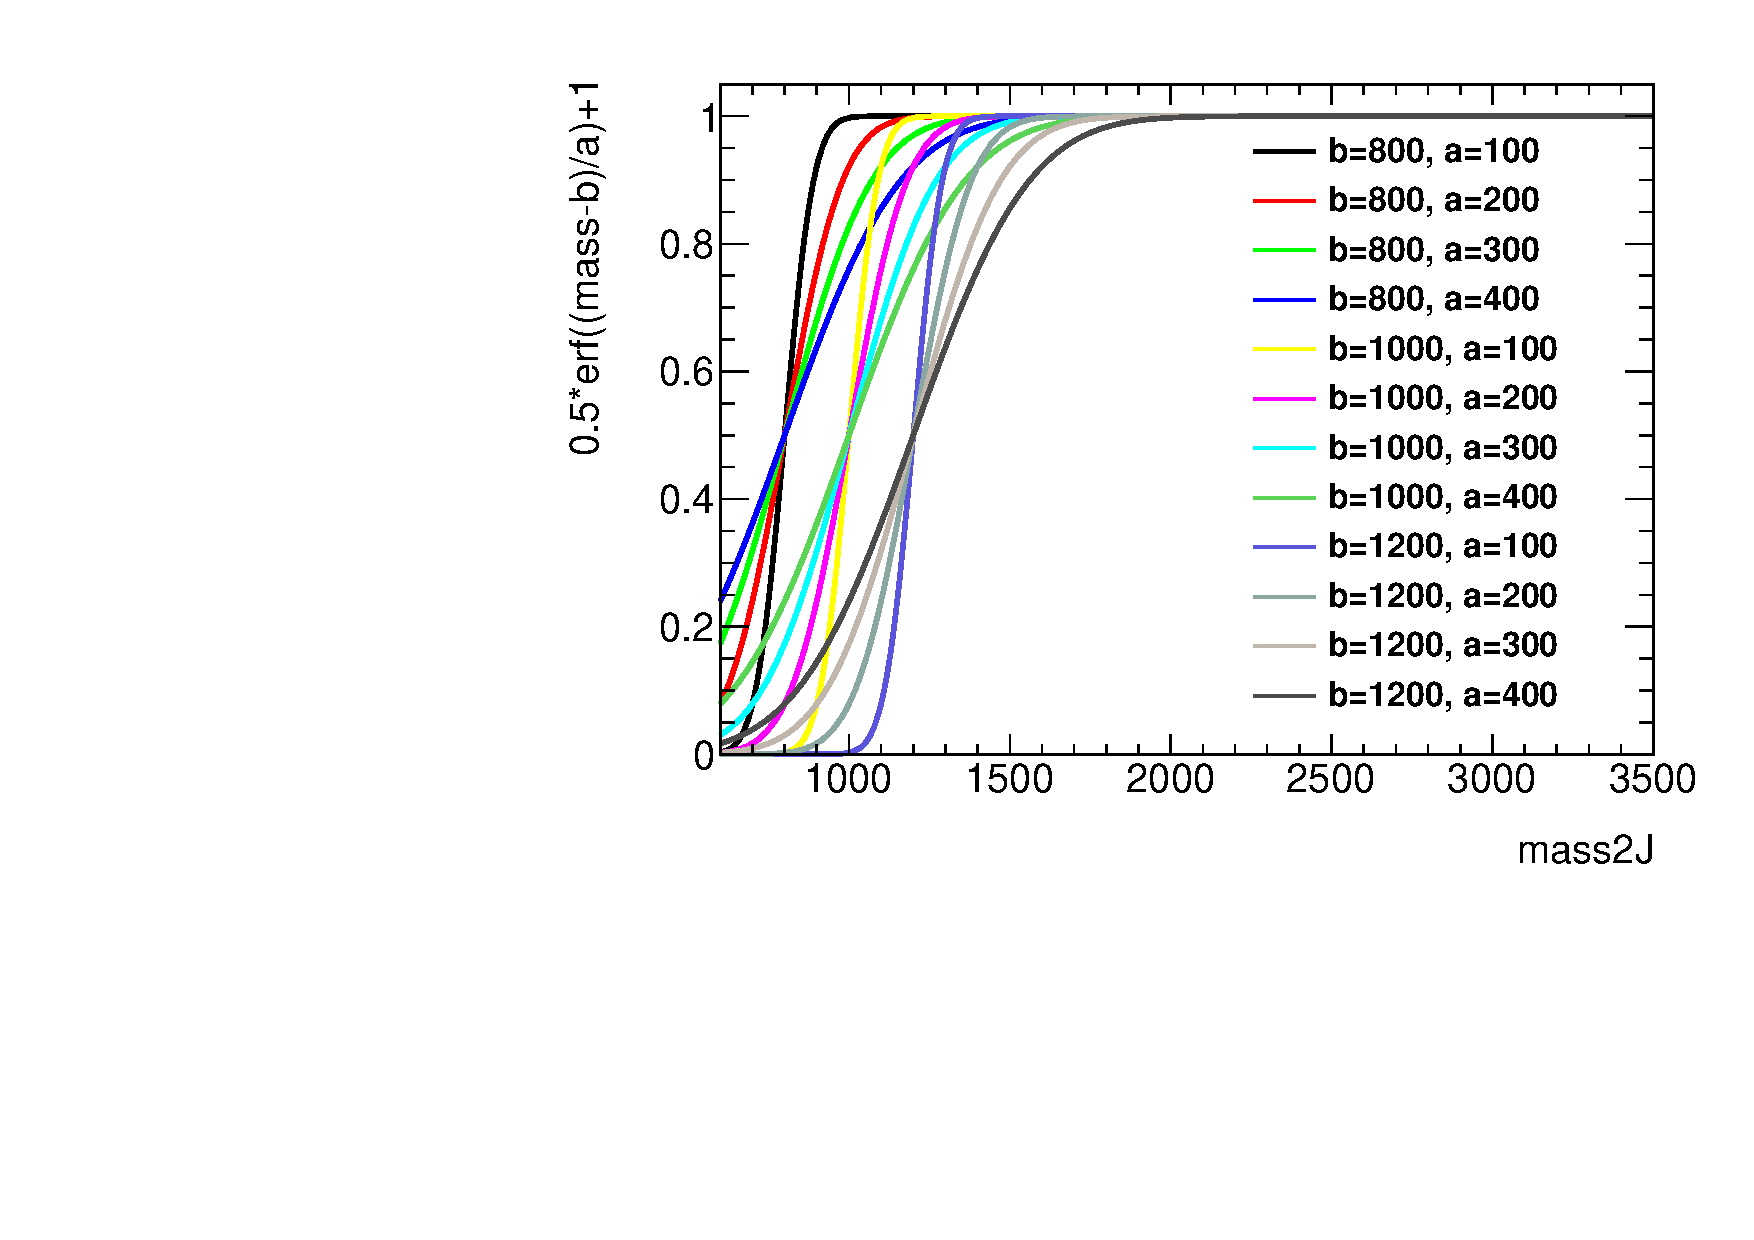
\includegraphics[angle=270, width=0.45\textwidth]{./figures/boosted/app-directfit/erf_parameters.pdf}
\caption{The shape of the error function for different values of parameters a and b.}
\label{fig:directfit:erf}
\end{center}
\end{figure*}

In a background-only fit, the parameters a and b float freely and the values are determined by the fit, given the parameter ranges are chosen reasonably. In a signal+background fit, howerver, it is found that the fit becomes unstable if the signal is close to the turn-on, and therefore the parameters a and b need to be constrained by Gaussians. In the latter case, the start values and uncertainties for a and b are determined in background-only fits and those values then used to define the constraints. With this approach, fit stability is assured.

\subsection{Signal Model}

The signal is modelled with MC samples generated at specific mass points. But it would be beneficial to have a model that describes the signal shape and the signal yield for any given value of the 2J mass. The first method that was attempted is to model the signal in the same way as it's done in the resolved analysis, using a Voigtian and an efficiency correction. Since this results in mis-modellings for high mass points, another method based on histogram morphing is tested. The latter method is then used for the spurious signal study. Shown here are Graviton (c=1) samples.

\subsubsection{Voigtian with Efficiency Correction}

The Voigtian is a Breit-Wigner convoluted with a Gaussian. It has three parameters: The mean (shared by both the Breit-Wigner and the Gaussian), the width of the Breit-Wigner (this is taken as the generated width of the MC samples, it depends on the mass point, it is a fixed parameter), and the sigma of the Gaussian. The mean and the sigma are determined from fits to the signal MC.
The efficiency corrections is the value of efficiency times acceptence as a function of the mass points, ie. the number of signal events passing the selection divided by the number of initial signal events. It is modelled with a spline. The efficiency corrections are shown in Fig.~\ref{fig:directfit:efficiencies}.
The total signal model is then a multiplication of the Voigtian with the efficiency.

\begin{figure*}[htbp!]
\begin{center}
\subfloat[]{ 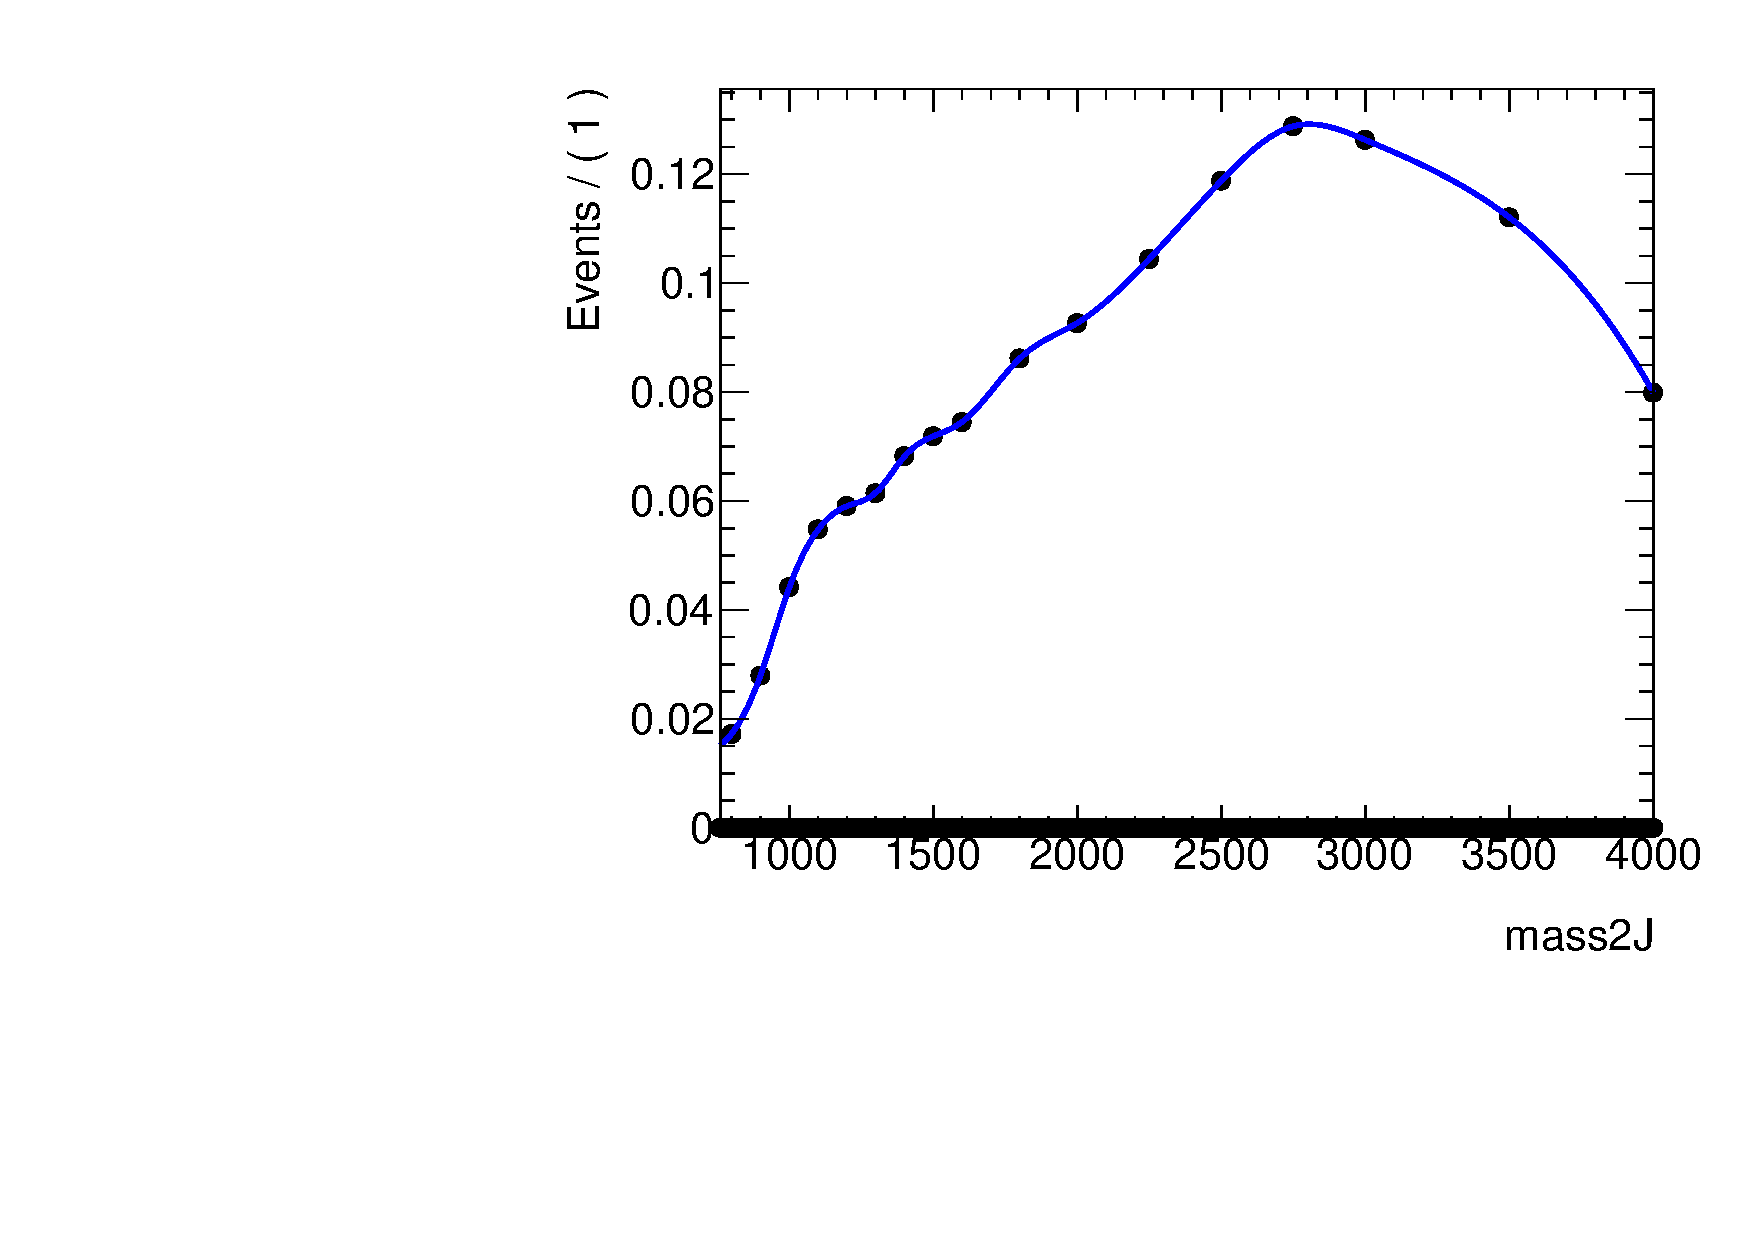
\includegraphics[angle=270, width=0.32\textwidth]{./figures/boosted/app-directfit/spline_tag2.pdf} }
\subfloat[]{ 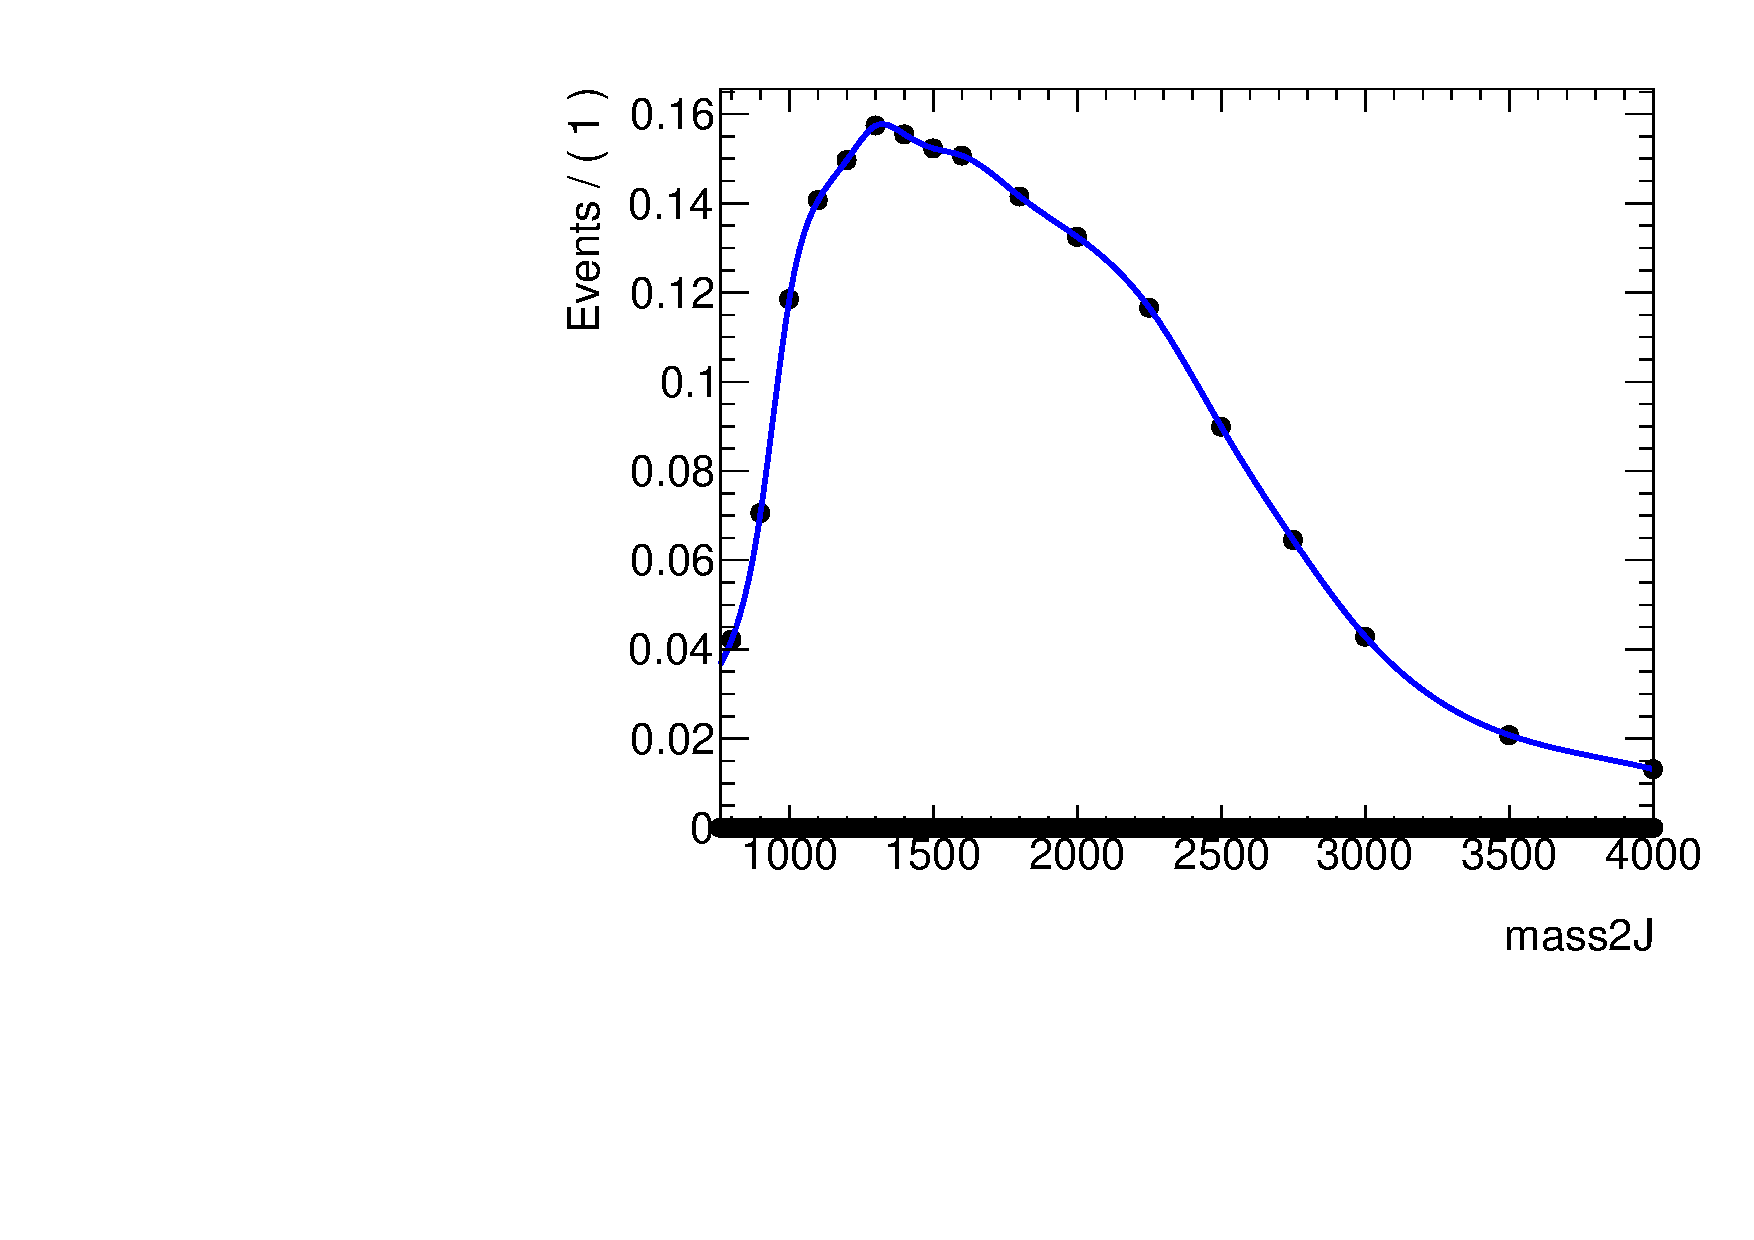
\includegraphics[angle=270, width=0.32\textwidth]{./figures/boosted/app-directfit/spline_tag3.pdf} }
\subfloat[]{ 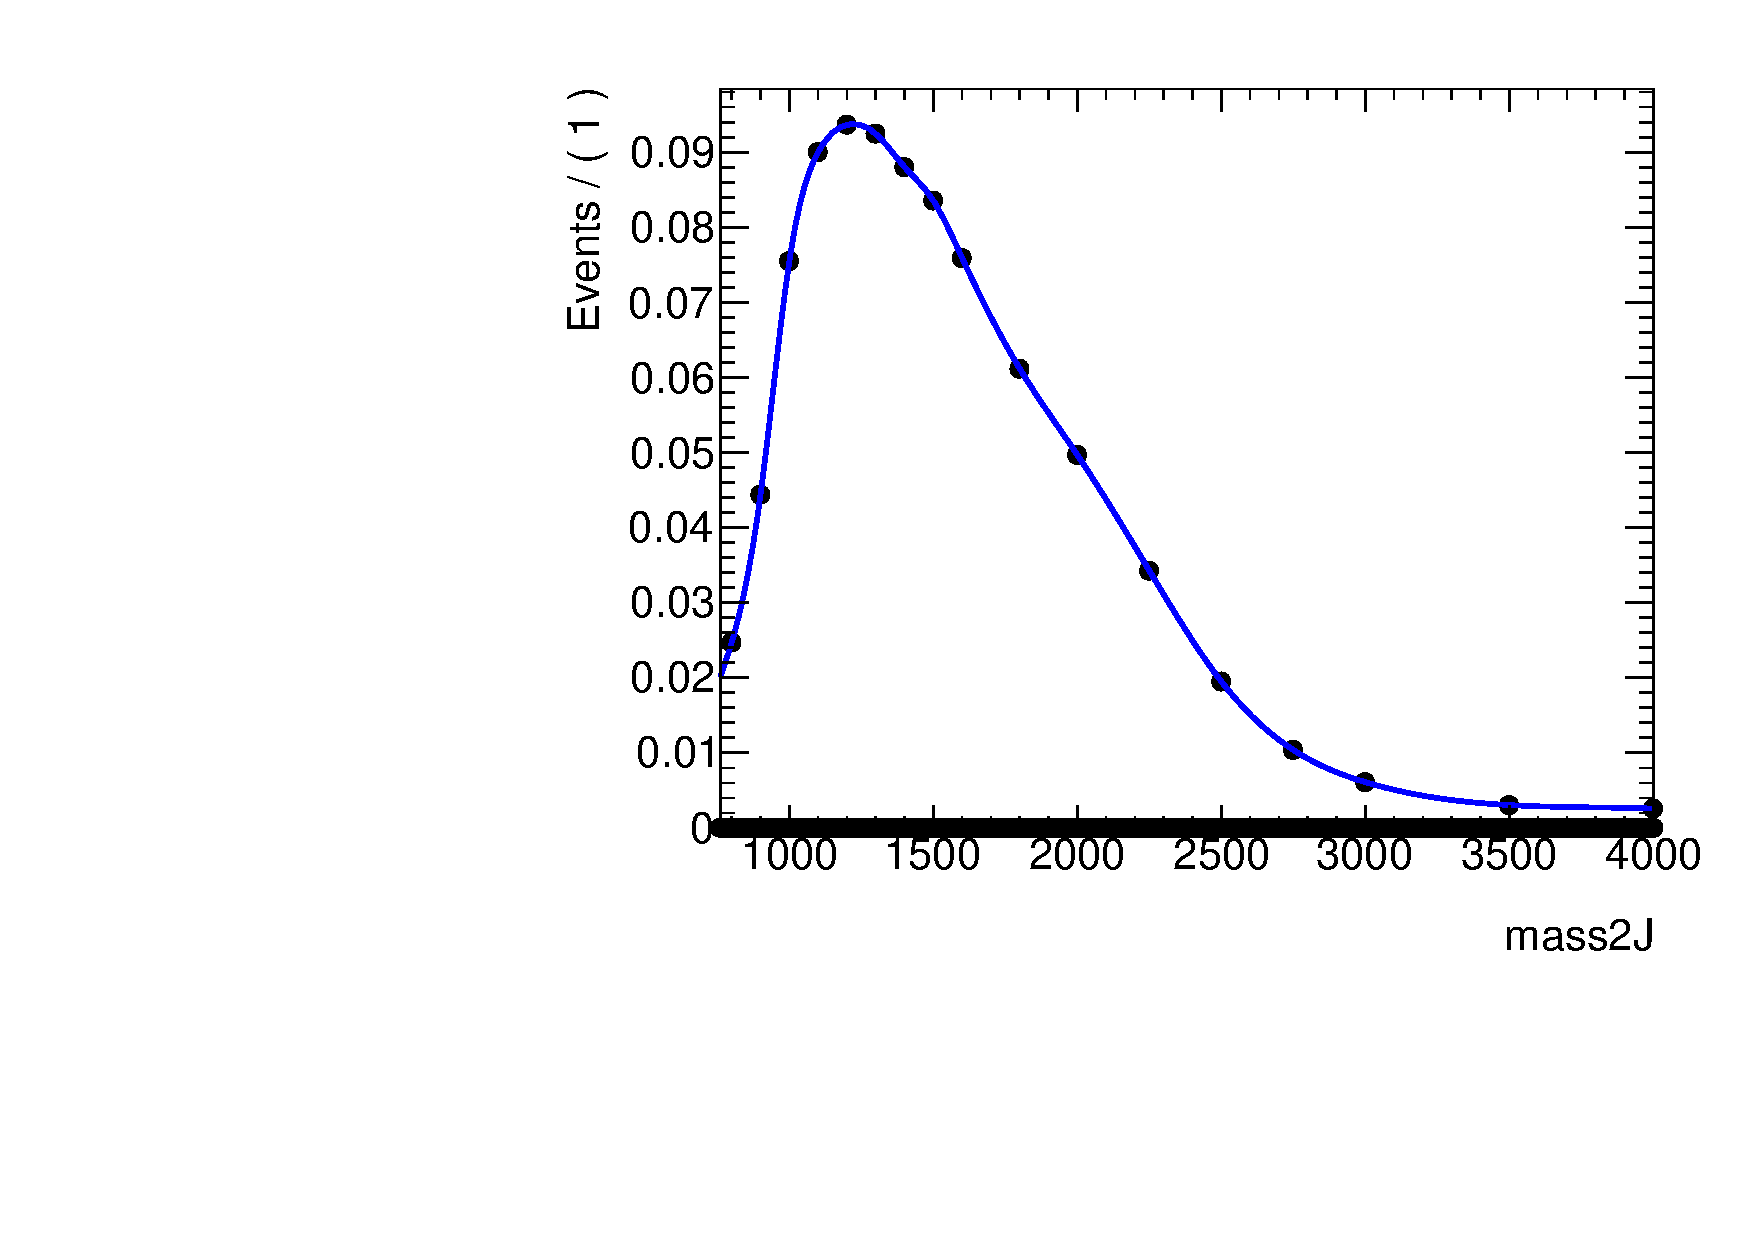
\includegraphics[angle=270, width=0.32\textwidth]{./figures/boosted/app-directfit/spline_tag4.pdf} }
\caption{Efficiency of signal events after the full selections wrt. the inital number of events, in (a) 2bs, (b) 3b and (c) 4b. The curve connecting the points is a spline of order three.}
\label{fig:directfit:efficiencies}
\end{center}
\end{figure*}

This method does well for masses below 2 TeV, but has limitations at high mass, especially in the 4b category. Some plots showing the signal mass and the modelling are displayed in Fig.~\ref{fig:directfit:signalmodel} and Fig.~\ref{fig:directfit:signalmodel3k}. There are some indications, that the usage of variable-radius track-jets instead of fixed-radius track jets will recover the 2J mass shape and then this modelling method might be useful. This needs to be checked in the future.

\begin{figure*}[htbp!]
\begin{center}
\subfloat[]{ 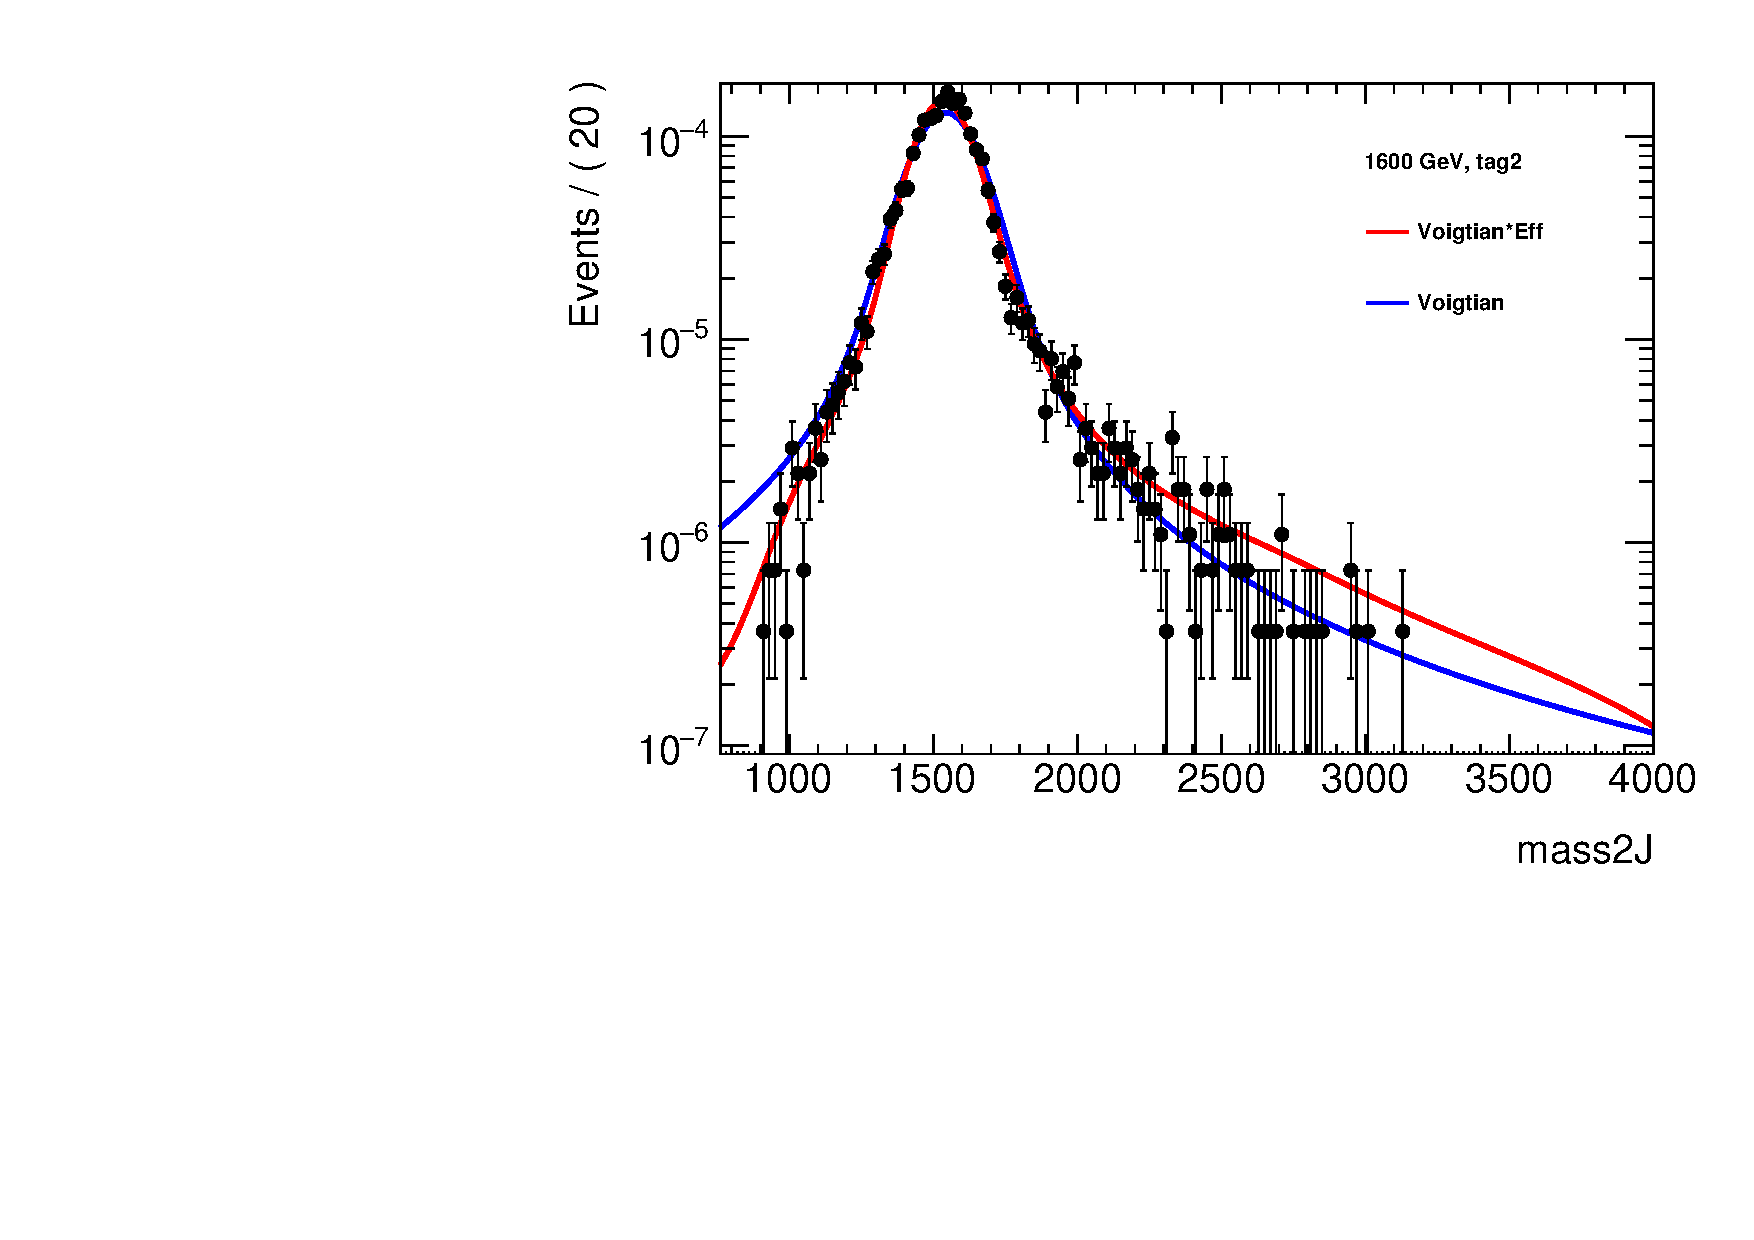
\includegraphics[angle=270, width=0.32\textwidth]{./figures/boosted/app-directfit/tag2_1600.pdf} }
\subfloat[]{ 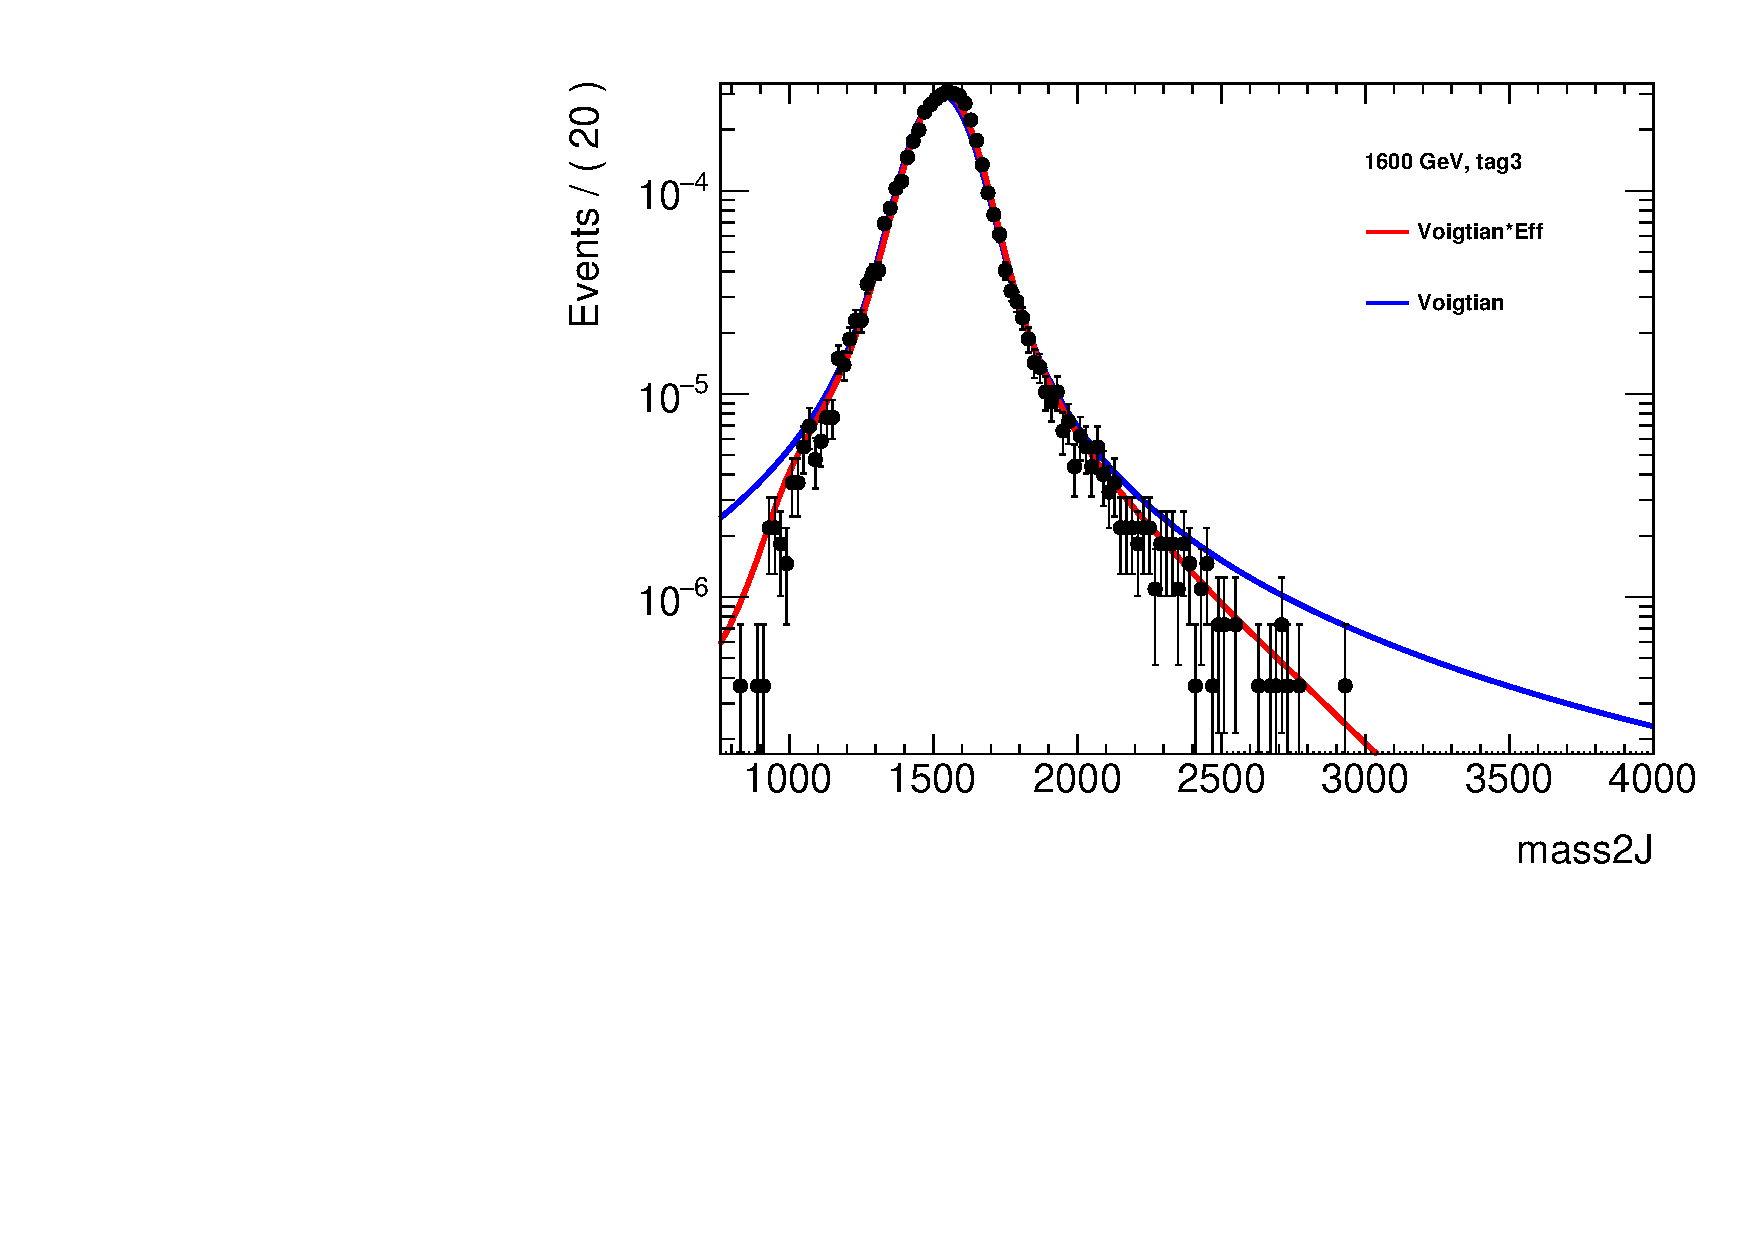
\includegraphics[angle=270, width=0.32\textwidth]{./figures/boosted/app-directfit/tag3_1600.pdf} }
\subfloat[]{ 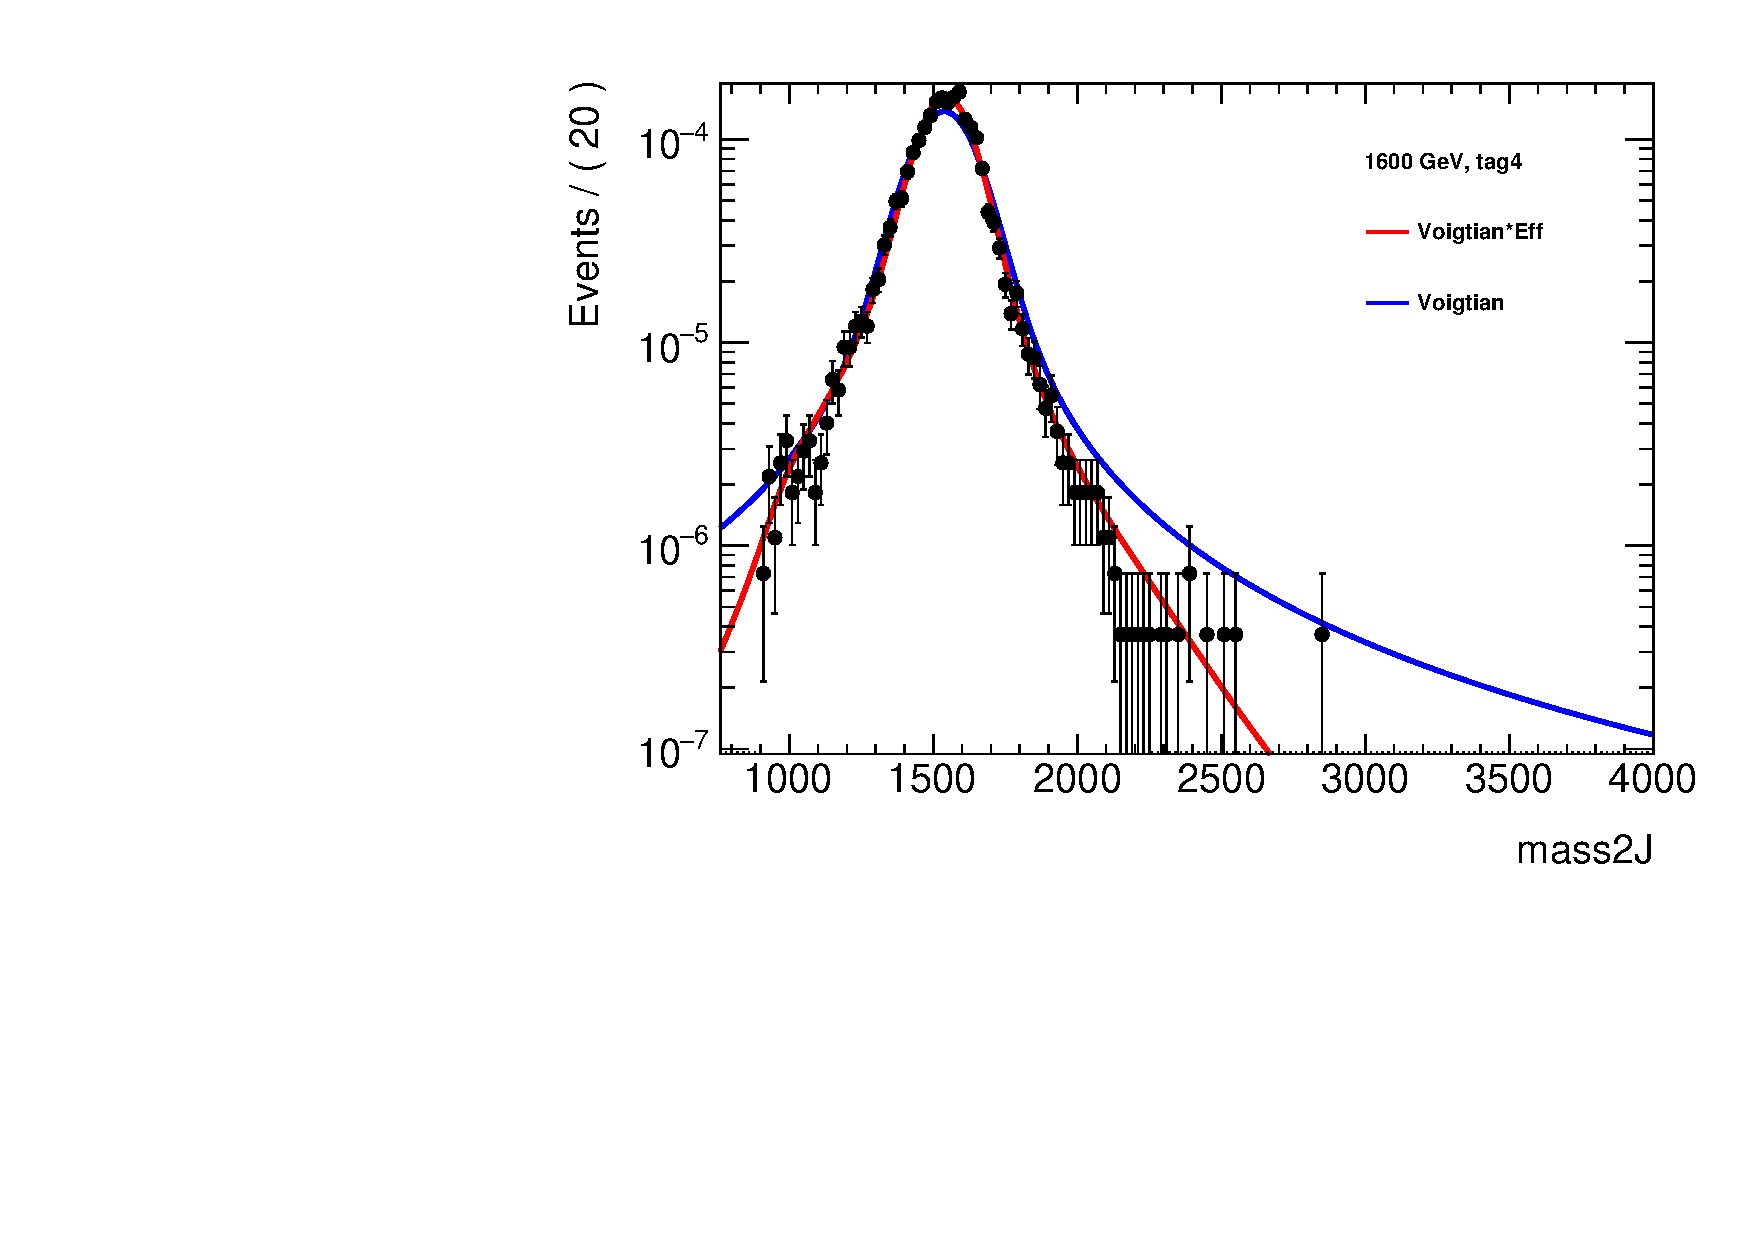
\includegraphics[angle=270, width=0.32\textwidth]{./figures/boosted/app-directfit/tag4_1600.pdf} }
\caption{The signal model for 1600 GeV in region (a) 2bs, (b) 3b and (c) 4b. The efficiency corrections improves the model.}
\label{fig:directfit:signalmodel}
\end{center}
\end{figure*}

\begin{figure*}[htbp!]
\begin{center}
\subfloat[]{ 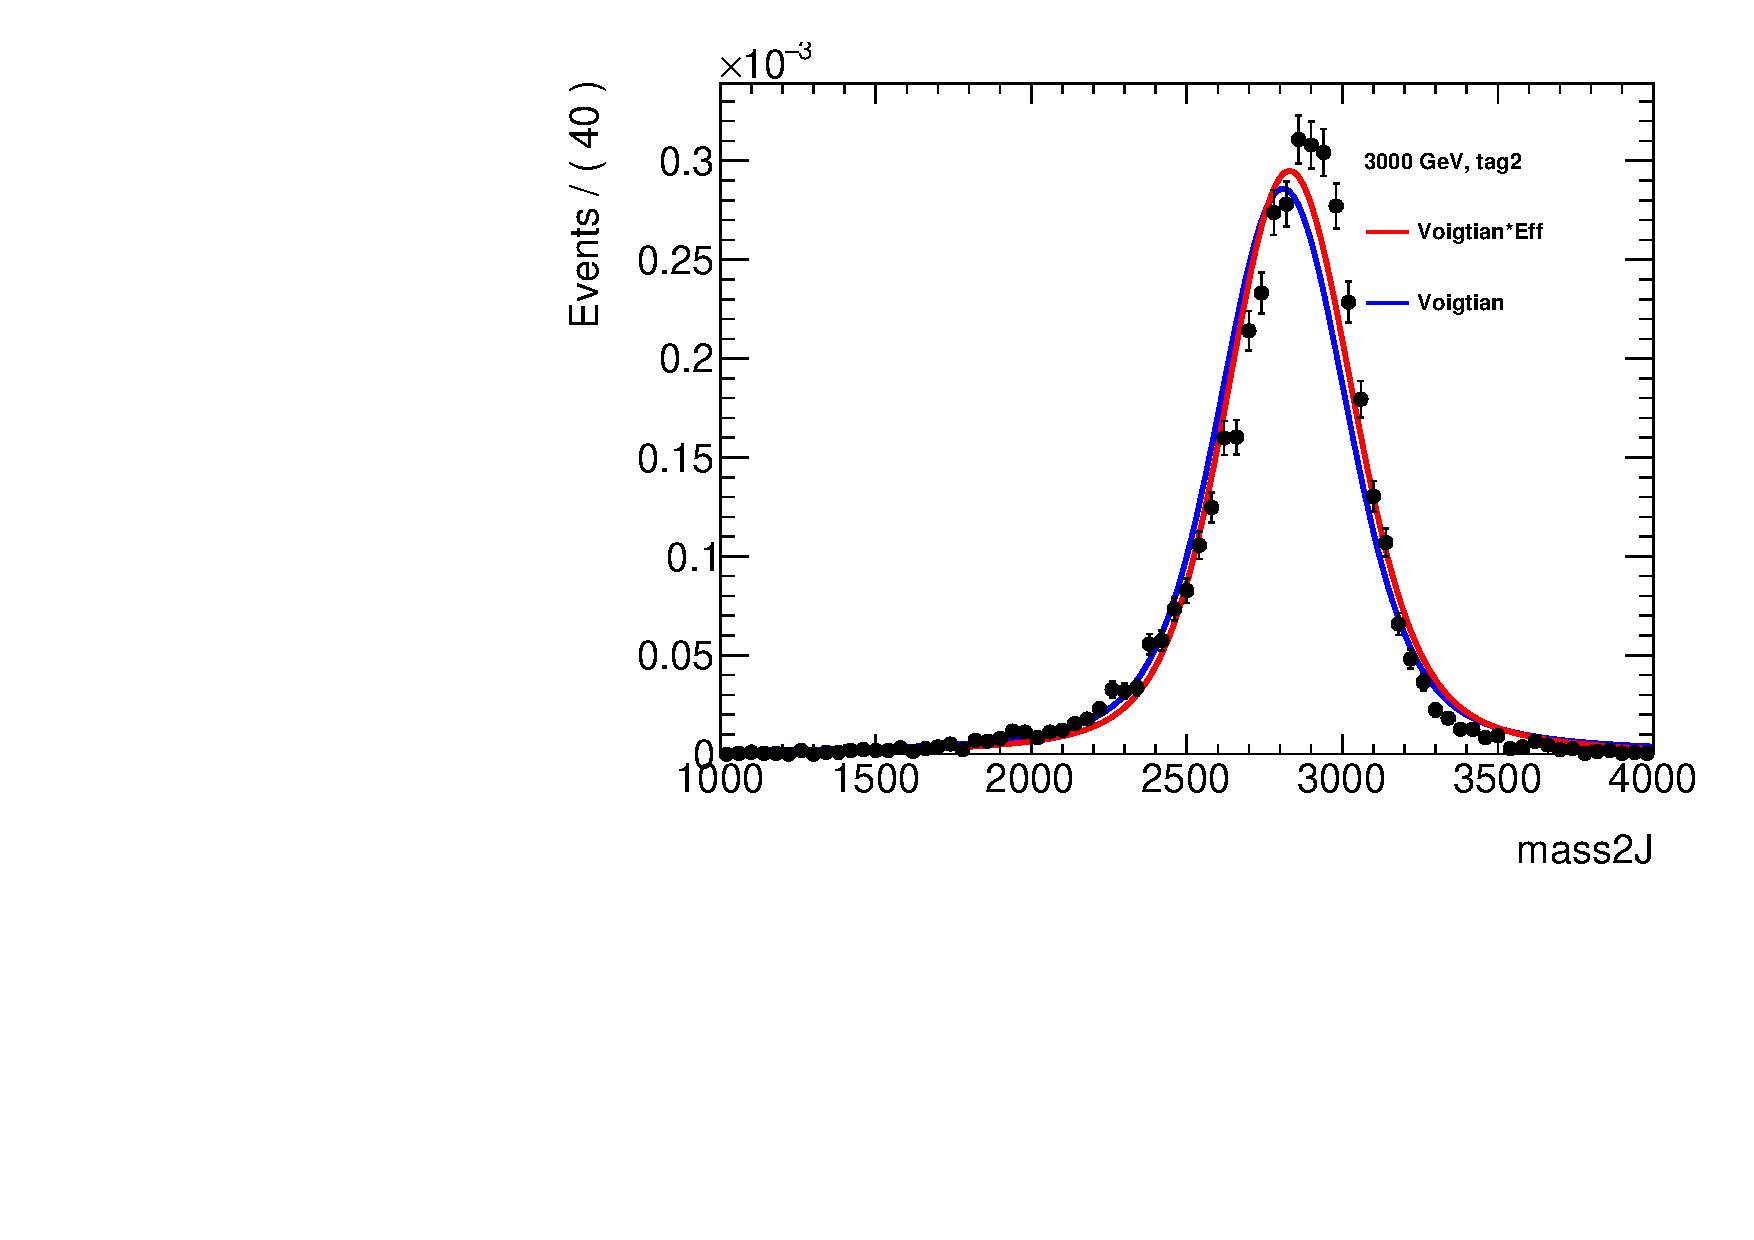
\includegraphics[angle=270, width=0.32\textwidth]{./figures/boosted/app-directfit/tag2_3000.pdf} }
\subfloat[]{ 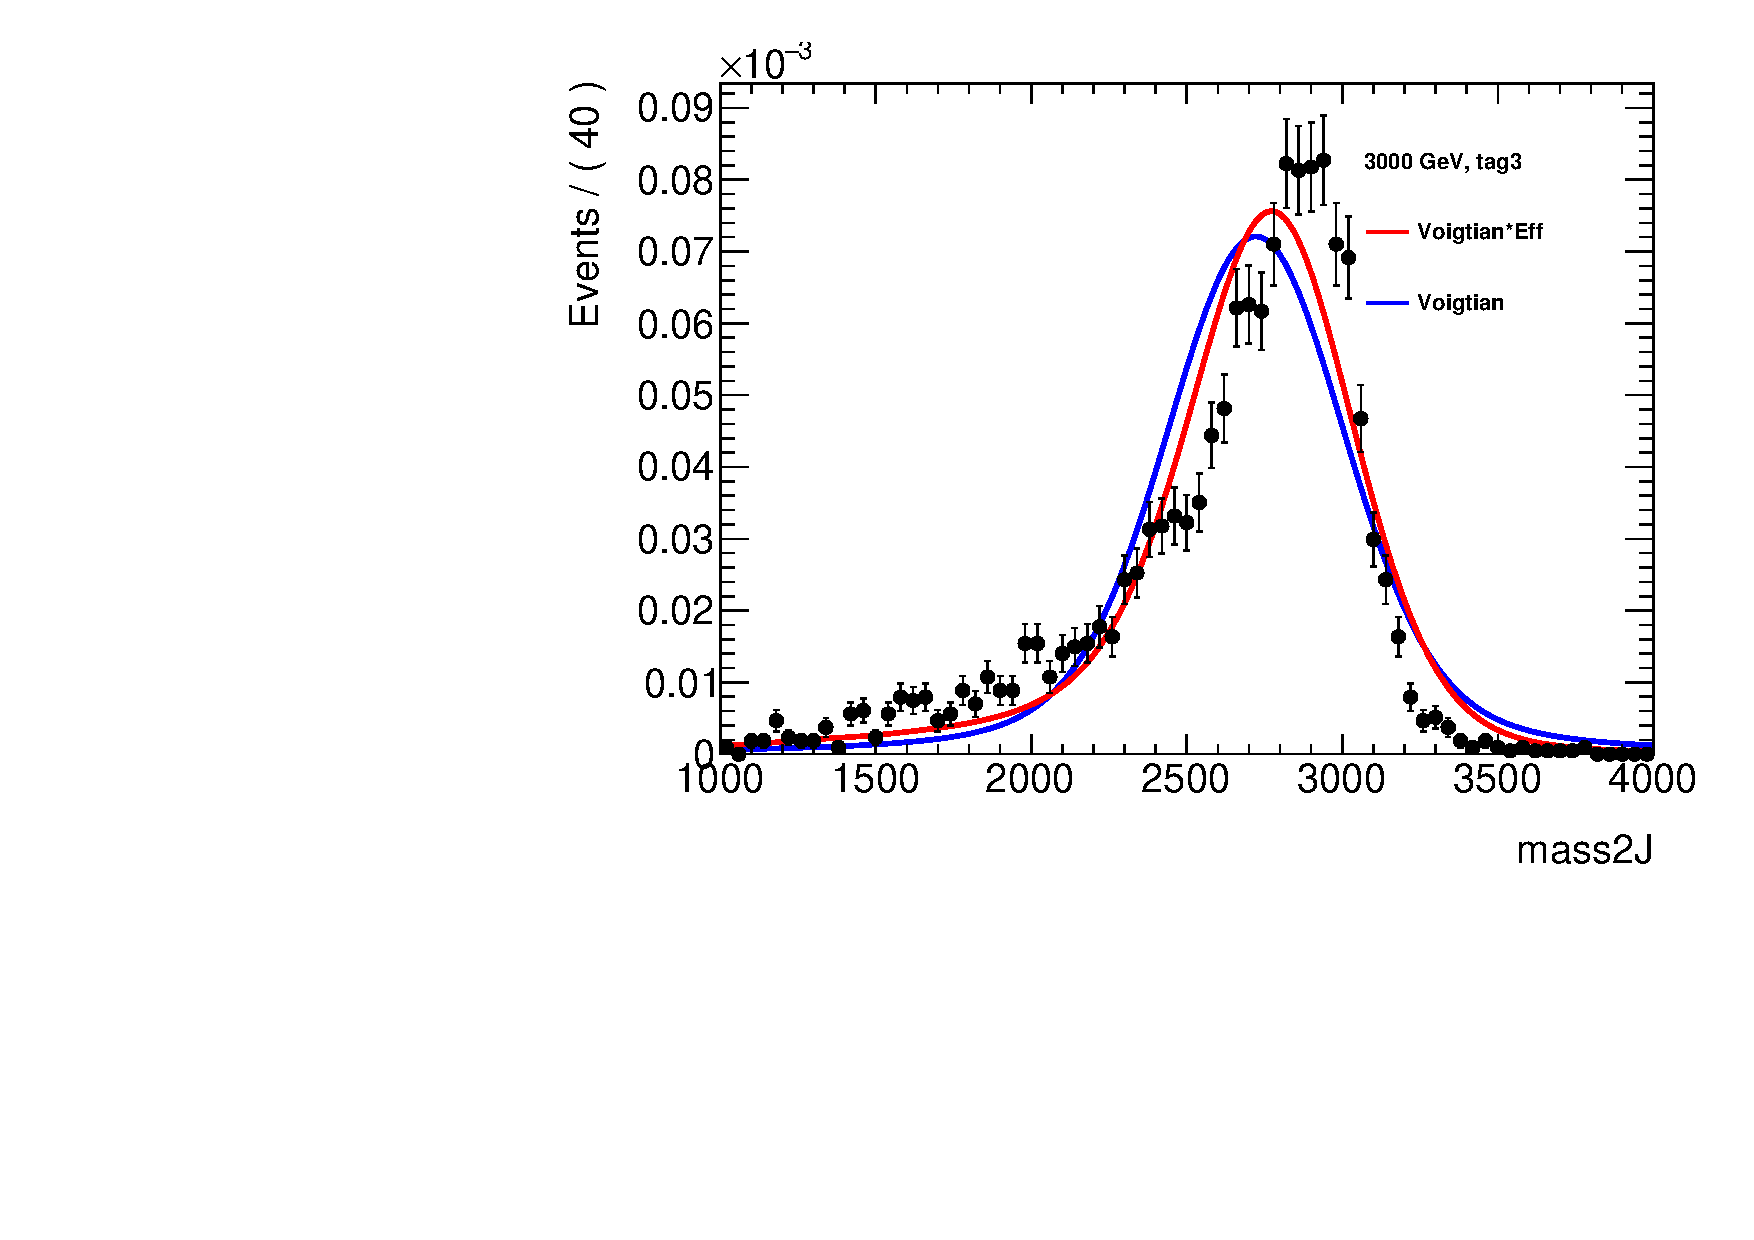
\includegraphics[angle=270, width=0.32\textwidth]{./figures/boosted/app-directfit/tag3_3000.pdf} }
\subfloat[]{ 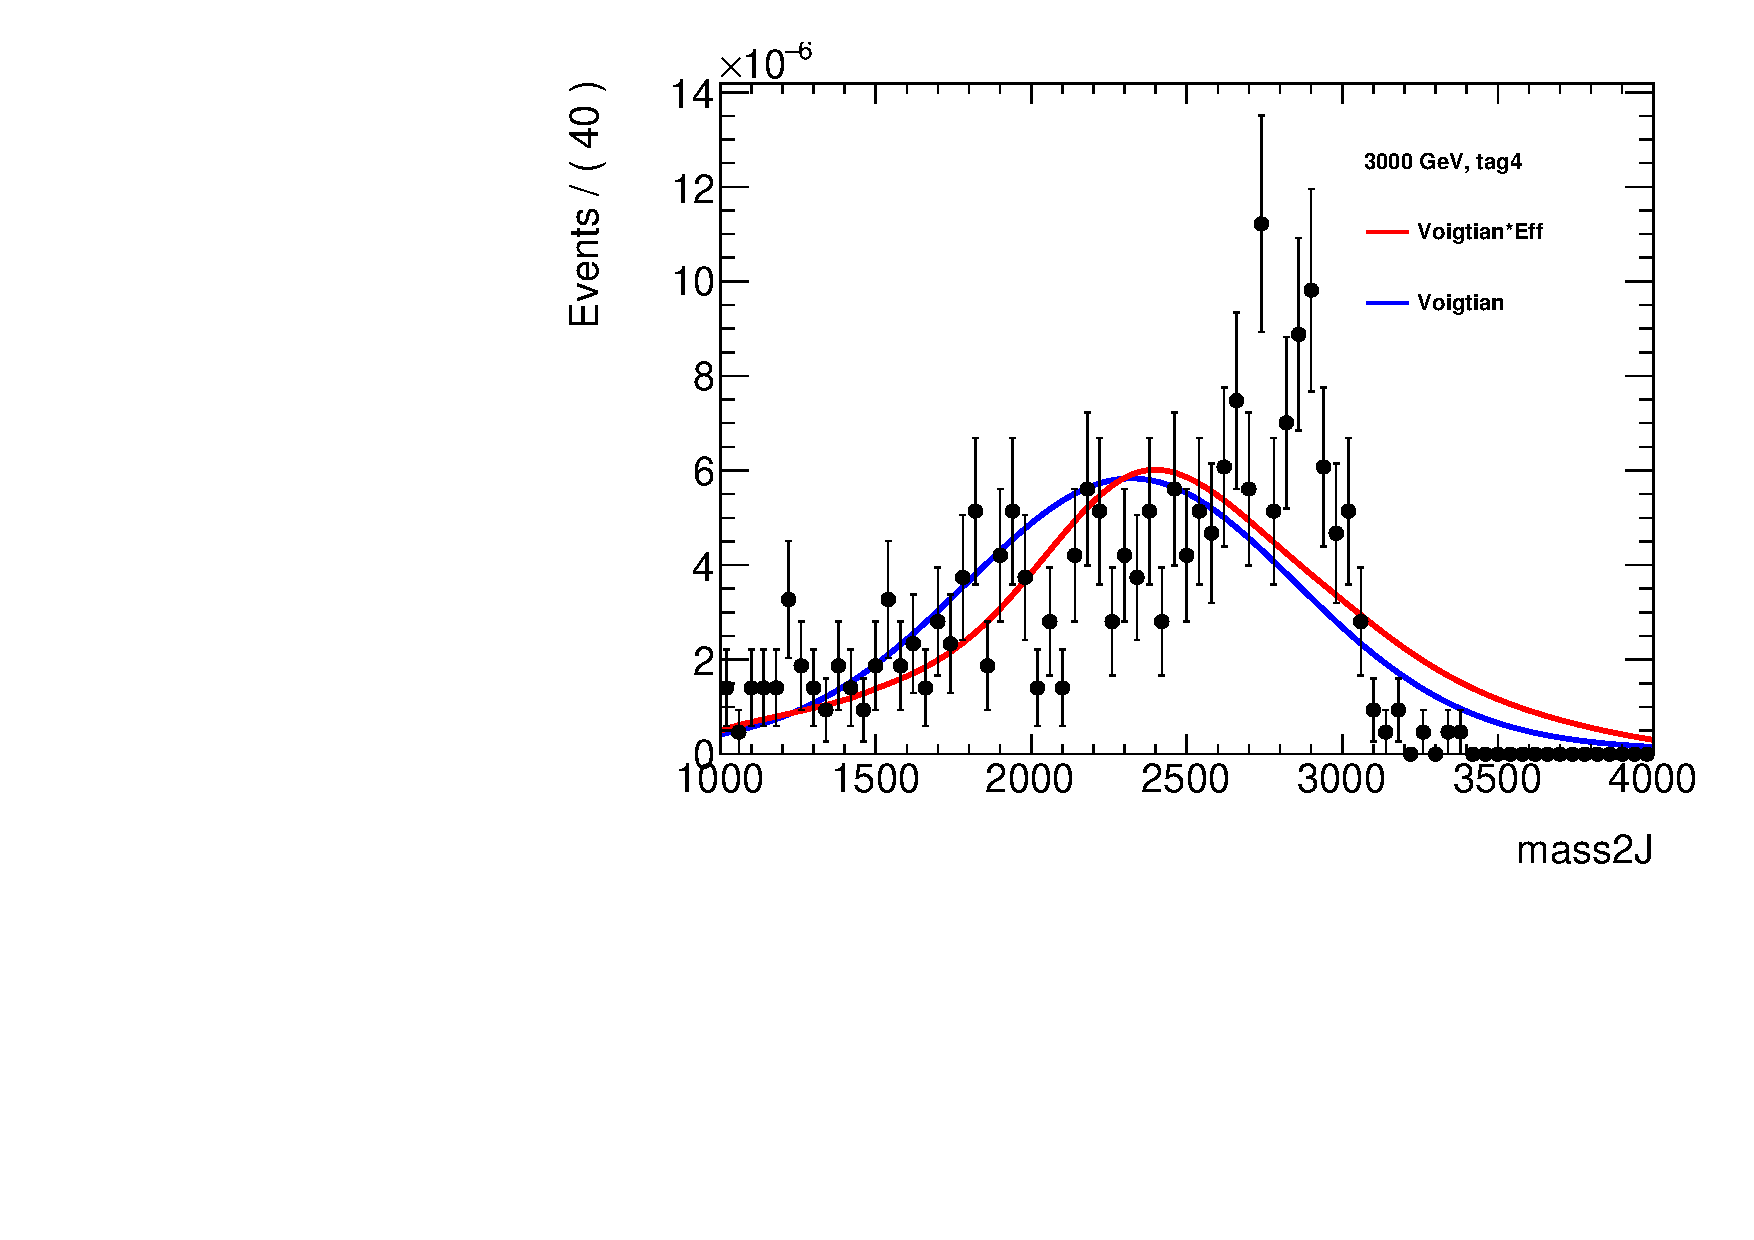
\includegraphics[angle=270, width=0.32\textwidth]{./figures/boosted/app-directfit/tag4_3000.pdf} }
\caption{The signal model for 3000 GeV in region (a) 2bs, (b) 3b and (c) 4b. The model fails at this mass. In particular in 4b, the signal shape is distorted.}
\label{fig:directfit:signalmodel3k}
\end{center}
\end{figure*}

\subsubsection{RooMomentMorph}

Since the analytical model fails, another method for a continous signal modelling is checked. The RooMomentMorph~\cite{roomomentmorph} is a method, where a morphing pdf is constructed from linear combination of template pdfs at fixed values of a morphing parameter. In our case, the Graviton mass is the morphing parameter. To test the performance, the 2750 GeV signal mass shape is obtained from morphing and overlayed with the signal MC at this mass, which is displayed in Fig.~\ref{fig:directfit:morphing}. The agreement is reasonable. In this test, the morphing is done over 500 GeV, while in the analysis the morphing is actually only done over 250 GeV. The morphing pdf is used as signal model throughout  the following studies. This, however, limits the statistical analysis to histogram-based approaches.

\begin{figure*}[htbp!]
\begin{center}
\subfloat[]{ 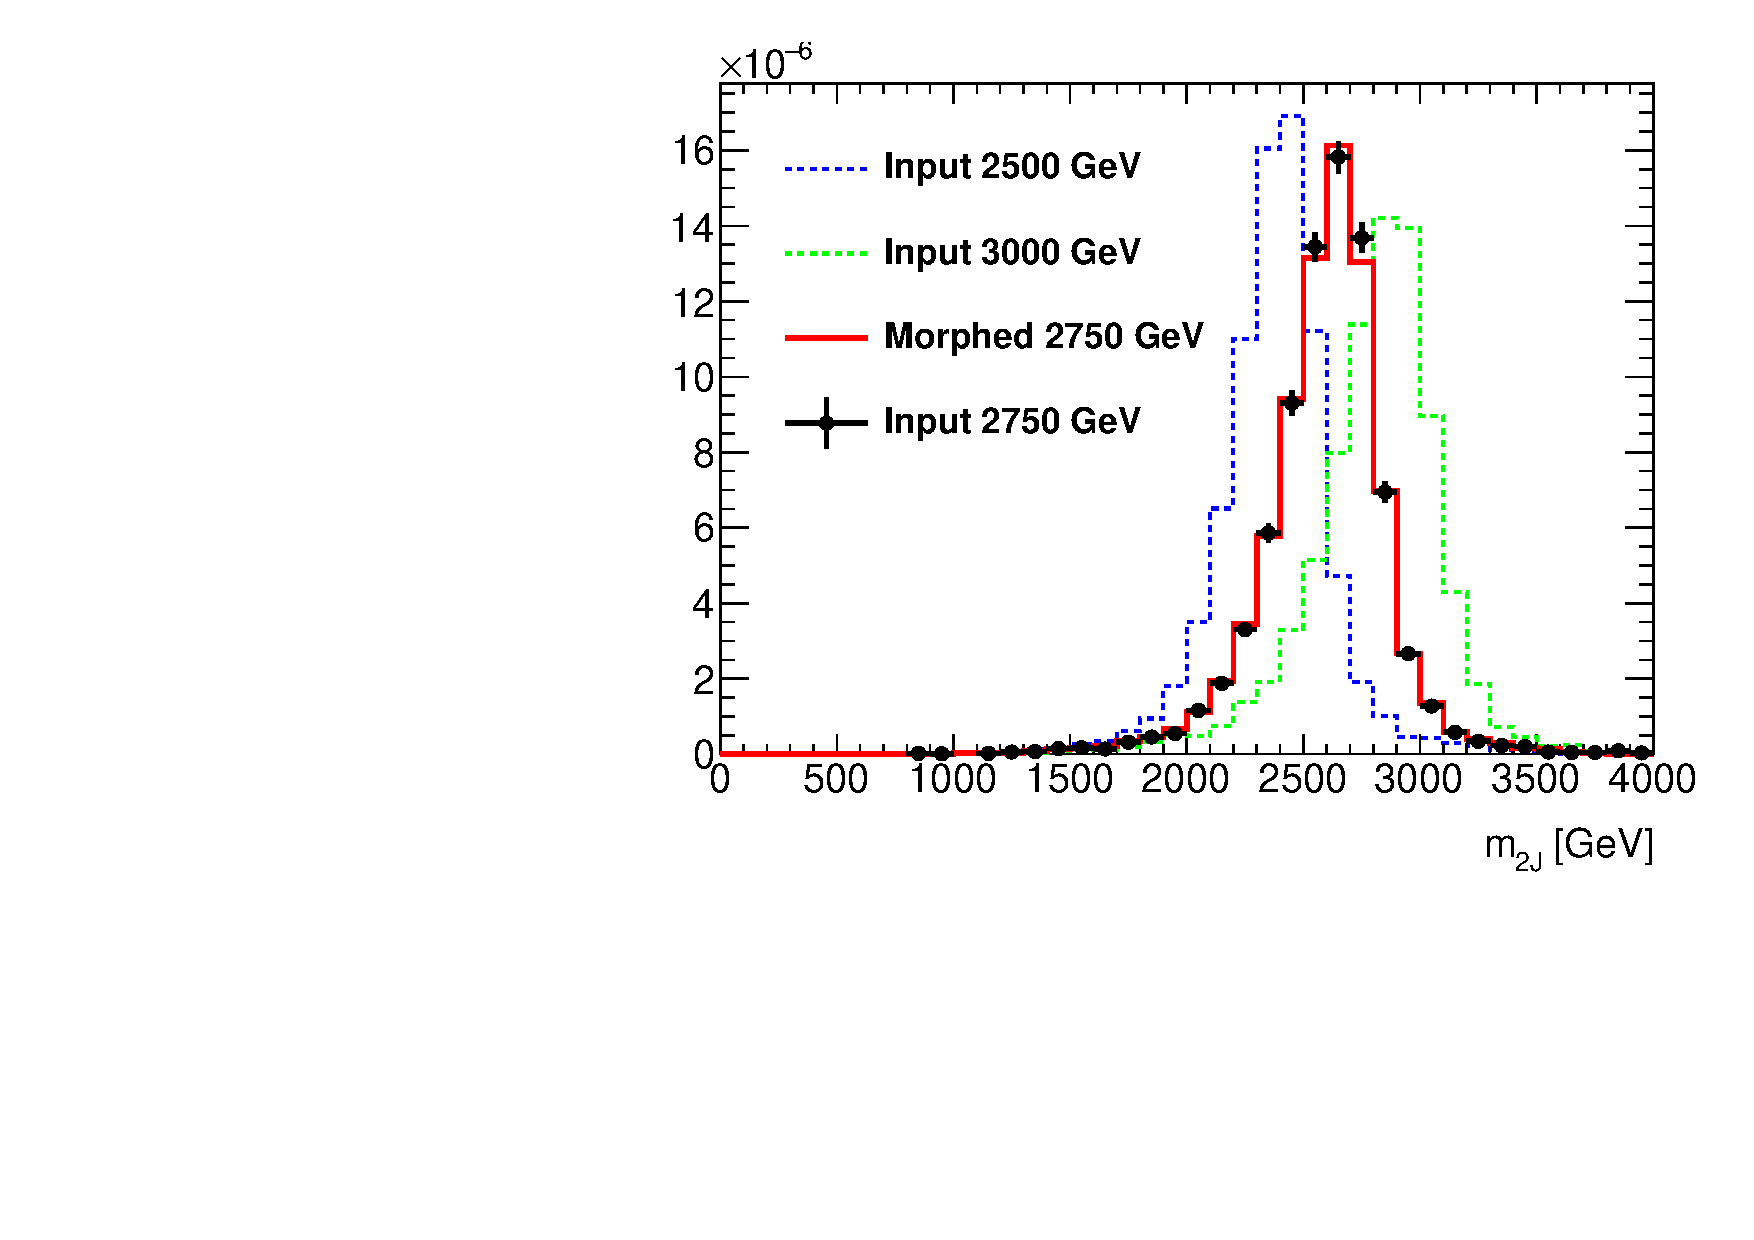
\includegraphics[angle=270, width=0.32\textwidth]{./figures/boosted/app-directfit/morph_tag2.pdf} }
\subfloat[]{ 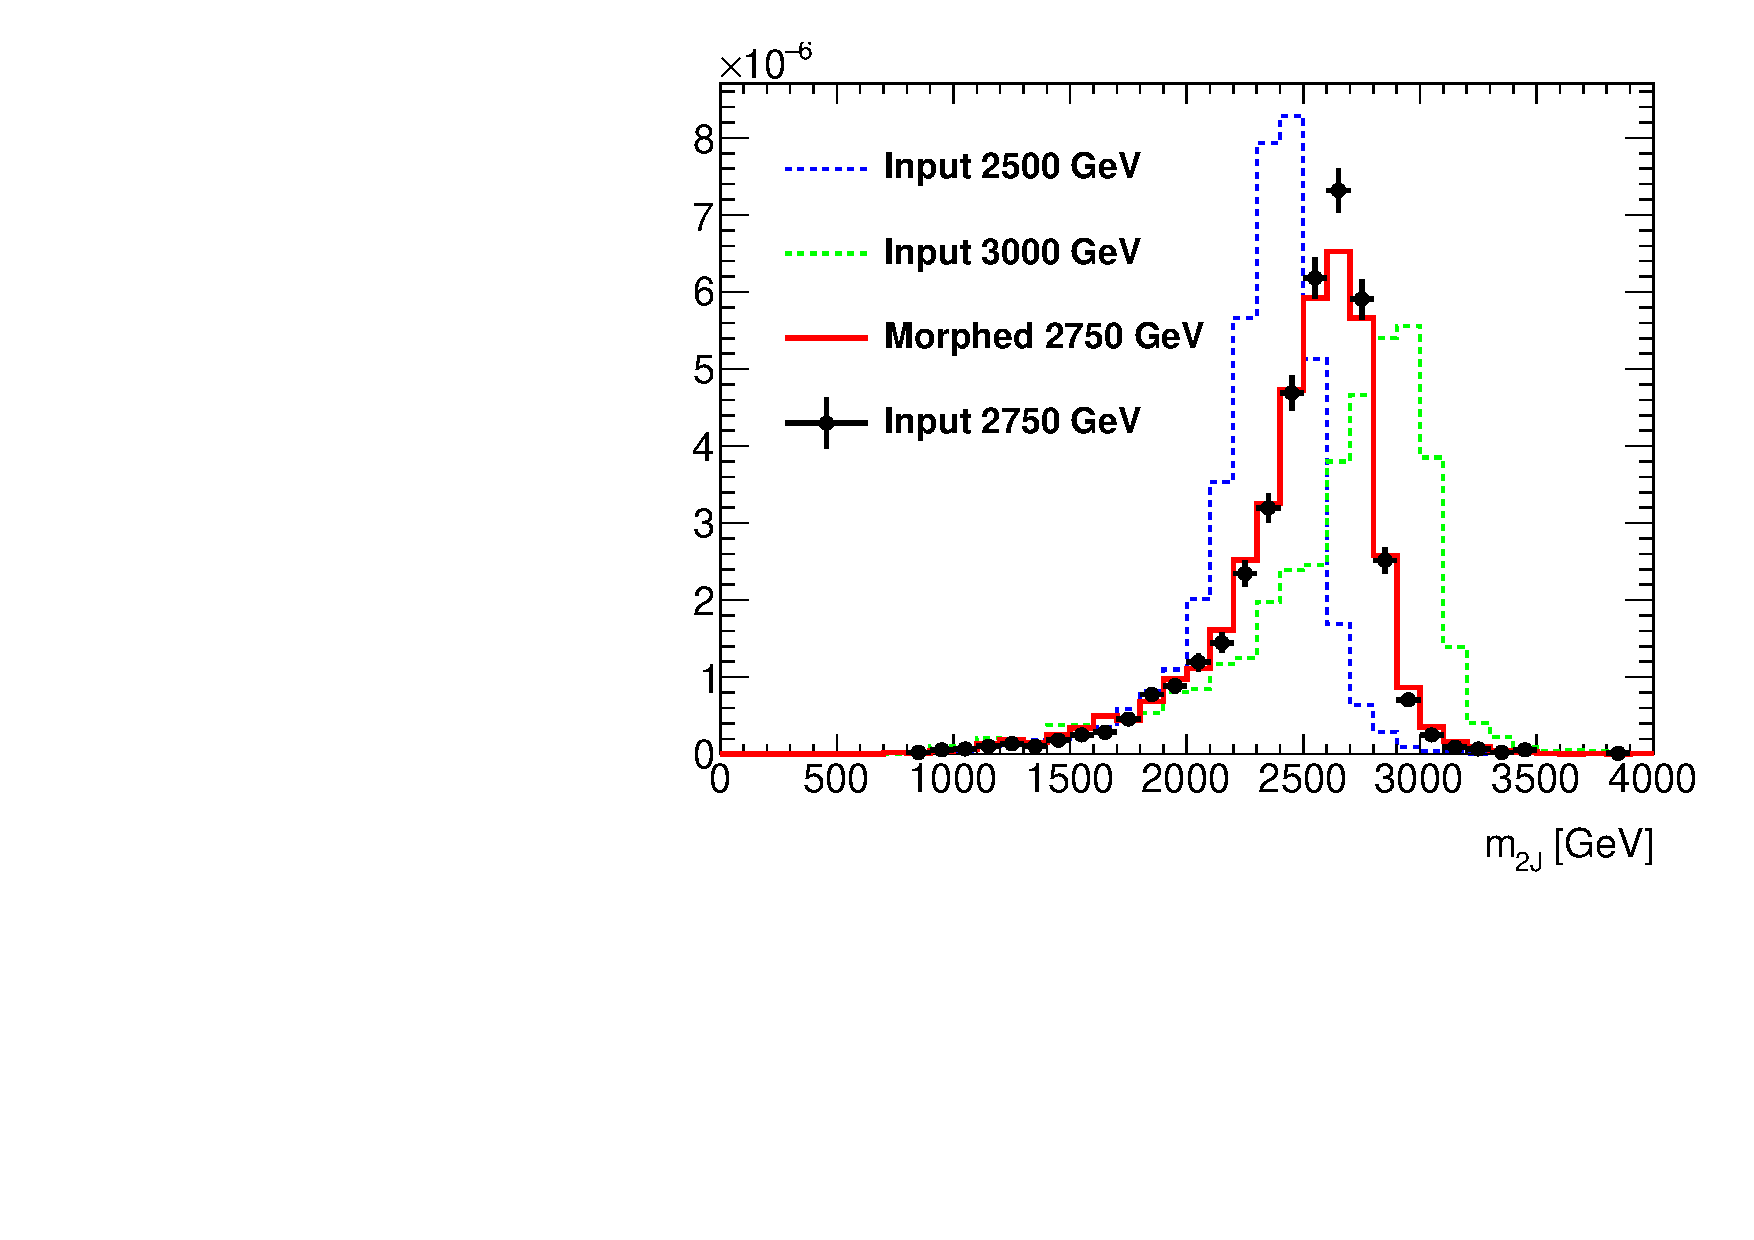
\includegraphics[angle=270, width=0.32\textwidth]{./figures/boosted/app-directfit/morph_tag3.pdf} }
\subfloat[]{ 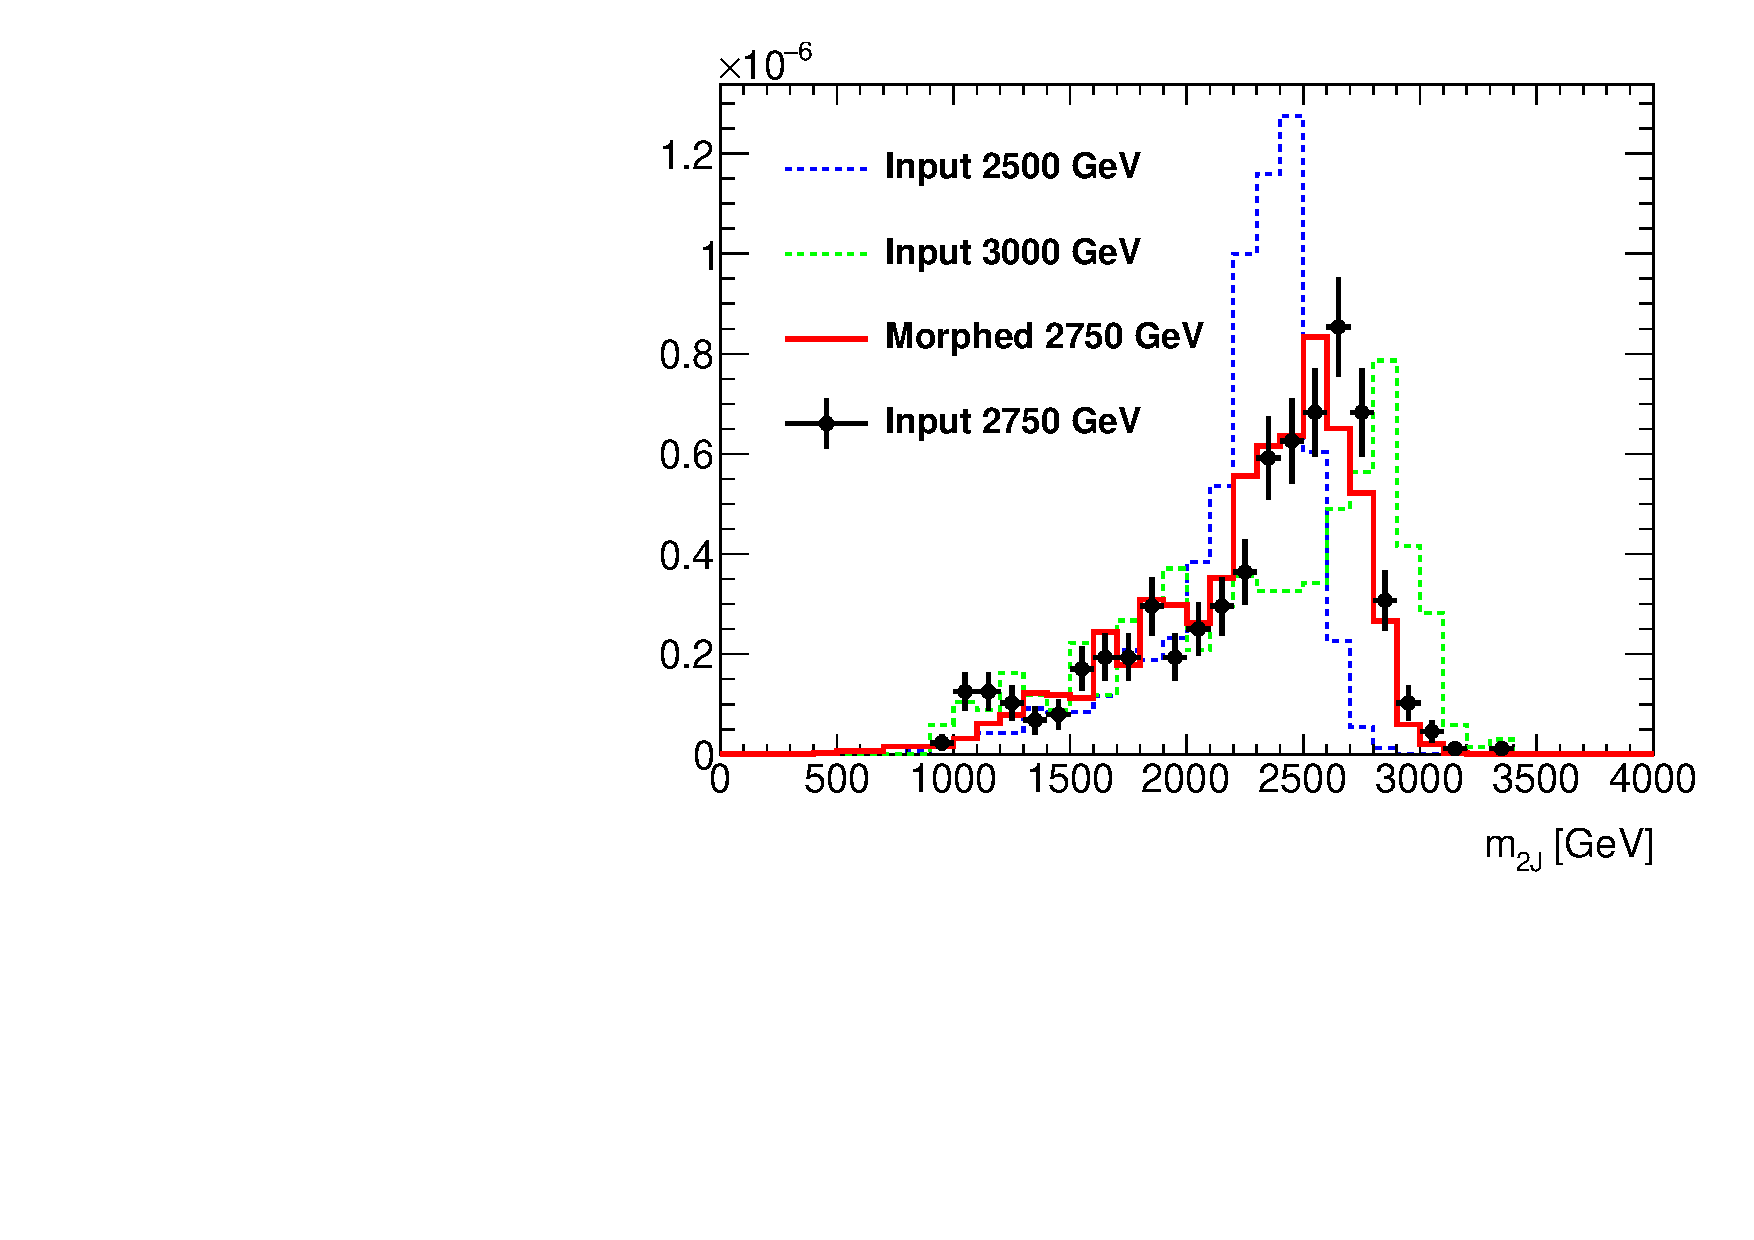
\includegraphics[angle=270, width=0.32\textwidth]{./figures/boosted/app-directfit/morph_tag4.pdf} }
\caption{The test of RooMomentMorph for the 2750 GeV masspoint in the (a) 2bs, (b) 3b and (c) 4b categories.}
\label{fig:directfit:morphing}
\end{center}
\end{figure*}


\subsection{Spurious Signal Study}

To find appropriate fit functions, a spurious signal study is performed. In this method, high-statistics signal-free background templates are fitted with the S+B model at a tight grid of signal masses. Since in the templates there is no real signal, any signal that is fitted, is instead a sign of a bias, ie. it quantifies directly the mismodelling of the background shape given the choice of function for the background.
The background templates are data obtained from lower-tagged signal regions, normalized to the data statistics in the actual signal regions, no reweighting is applied. The list of tested background models is as follows:

\begin{itemize}
\item Dijet functions:
\begin{itemize}
\item MJ1: $p_0 (1-x)^{p_1} x^{p_2}$
\item MJ2: $p_0 (1-x)^{p_1} e^{p_2 x^2}$
\item MJ3: $p_0 (1-x)^{p_1} x^{p_2 x}$
\item MJ4: $p_0 (1-x)^{p_1} x^{p_2 ln(x)}$
\item MJ5: $p_0 (1-x)^{p_1} (1+x)^{p_2 x}$
\item MJ6: $p_0 (1-x)^{p_1} (1+x)^{p_2 ln(x)}$
\item MJ7: $\frac{p_0}{x} (1-x)^{p_1-p_2 ln(x)}$
\item MJ8: $\frac{p_0}{x^2} (1-x)^{p_1-p_2 ln(x)}$
\end{itemize}
\item Bernstein polynomials 2-10th order
\item Single exponential
\item Exponential of a polynomial of 2-4th order, ie. $exp\left(a+bx+cx^2+..\right)$
\item Landau function
\item Sum of two dijet functions, Novosibirsk function, sum of Novosibirsk and dijet function
\end{itemize}

All those models are tested either by themselves, or in a product with the turn-on function.
The fit ranges are also varied. Since the turn-on is a problem appearing only at the beginning of the spectrum, but being largely irrelevant for the tail of the mass spectrum, it is also investigated how much a split into low and high mass fit can be useful. The entire documentation of all the tests that were done goes too far. It was found that MJ8 gave the best result (lowest spurious signal) on average, and that splitting the 2bs and 3b categories into low and high mass regions helps to control the background. In the 4tag region, the data statistics is so low, that a bias from the choice of function does not really matter. Here is the best result of the spurious signal study summarized:

\begin{itemize}
\item Category 2bs, low mass: $f_{TO}\cdot MJ8$ in fit range 950-2200 GeV, evaluation range 1200-2000 GeV
\item Category 2bs, high mass: $MJ8$ in fit range 1150-4000 GeV, evaluation range 2000-3000 GeV
\item Category 3b, low mass: $f_{TO}\cdot MJ8$ in fit range 950-2200 GeV, evaluation range 1200-2000 GeV
\item Category 3b, high mass: $MJ8$ in fit range 1300-4000 GeV, evaluation range 2000-3000 GeV
\item Category 4b: $f_{TO}\cdot MJ8$ in fit range 950-4000 GeV, evaluation range 1200-3000 GeV
\end{itemize}

This means, that for 2bs and 3b the fit function changes at 2000 GeV. This will be visible as a crack in the limit plot. The sensitivity will be evaluated using both the low and high mass functions at 2000 GeV, to assure the limit connects.

The spurious signal for this configuration is shown in Fig.~\ref{fig:directfit:nspurious}. The S+B fit to the background templates for the mass point where the spurious sginal is the largest, is shown in Fig.~\ref{fig:directfit:splubfitplots}.

In the Higgs group, a criteria is formulated for deciding which functions are good and which are bad. The criteria are that the spurious signal must be smaller than 20\% of the fitted signal uncertainty (which should correspon to the expected background uncertainty of the background below the signal), or smaller than 10\% of the expected signal yield. In this search, the signal yield depends on the BSM model, and in general it is very small, therefore only the former criterium is used as a guideline here. The remaining spurious signal measured at each mass point, is taken as a systematic uncertainty. This is the only background systematic uncertainty connected with the direct fit method (uncertainties on the fit parameters estimated during the fitting procedure are statistical in nature).

\begin{figure*}[htbp!]
\begin{center}
\subfloat[]{ 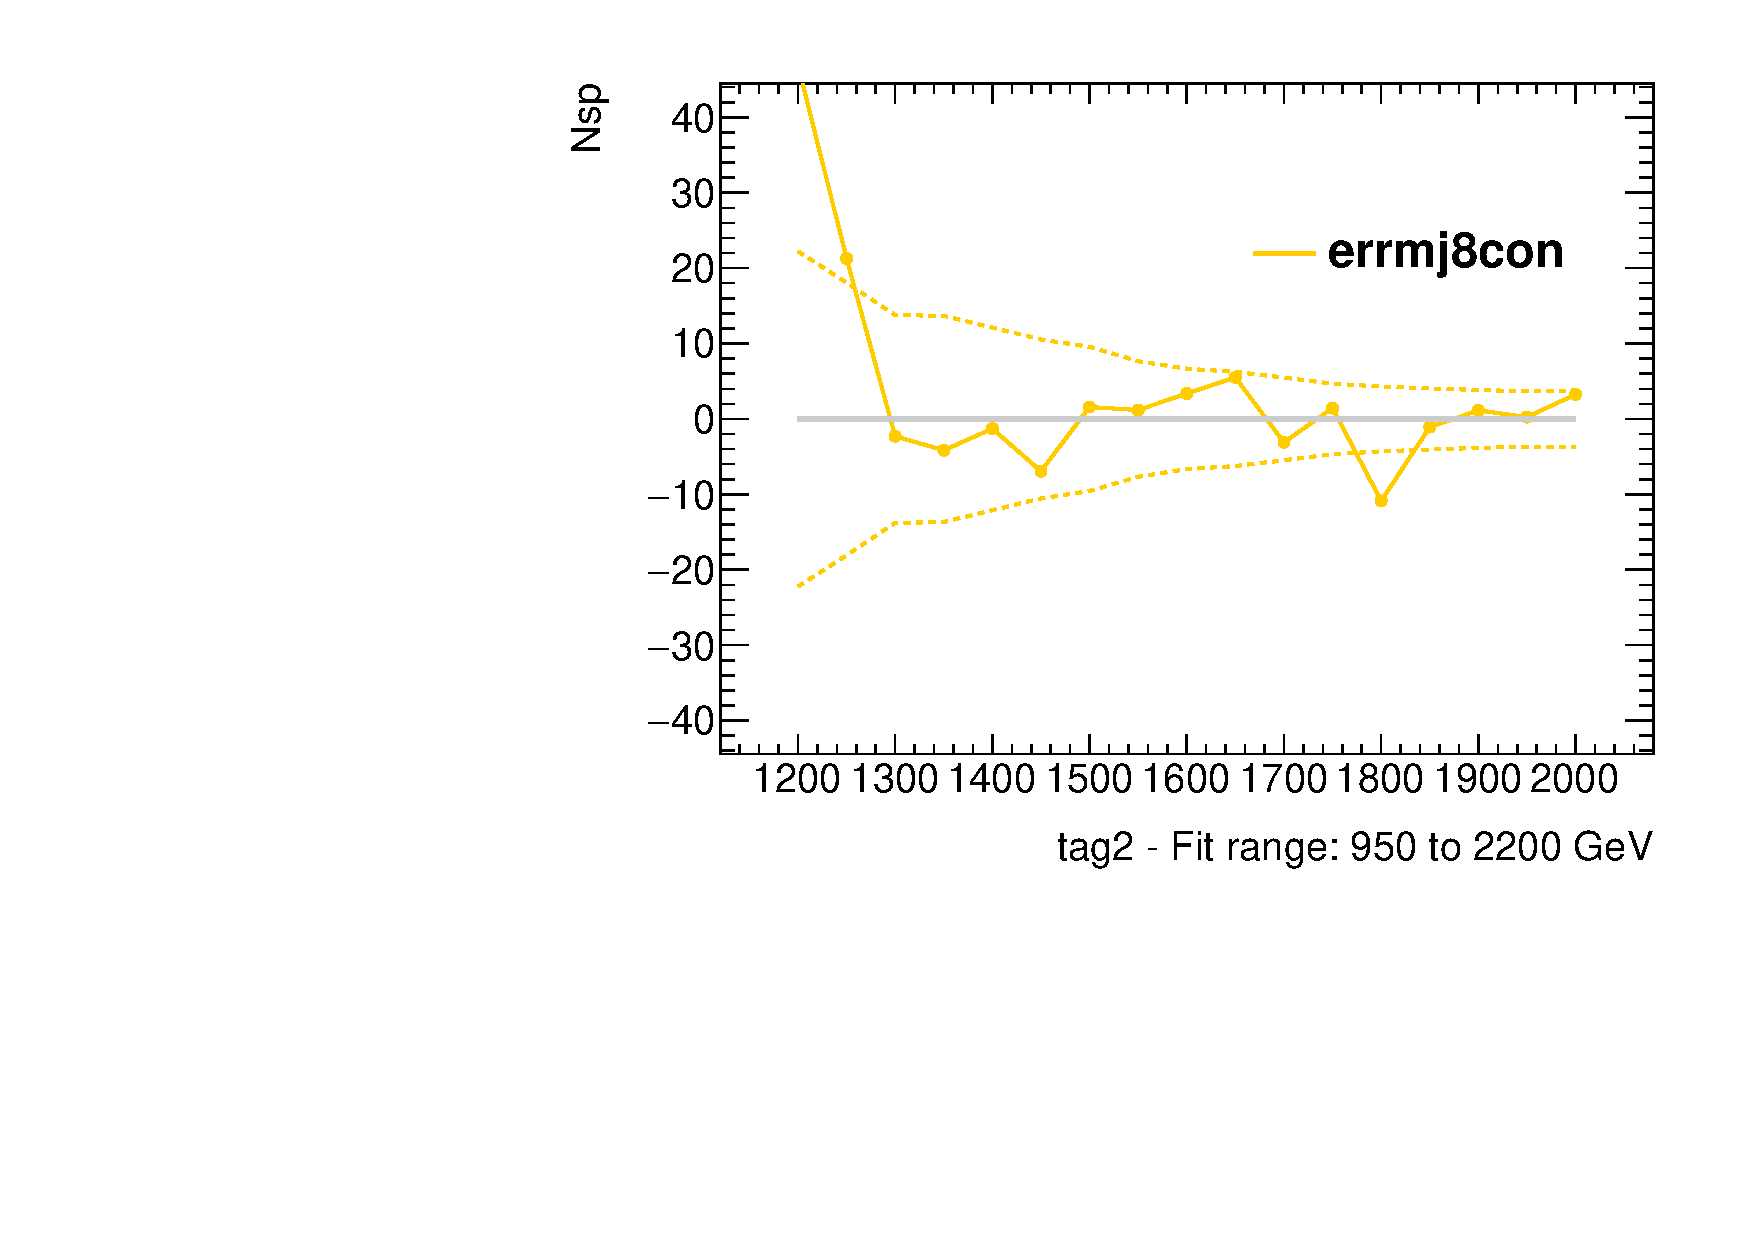
\includegraphics[angle=270, width=0.32\textwidth]{./figures/boosted/app-directfit/Nsp_tag2_range950to2200.pdf} }
\subfloat[]{ 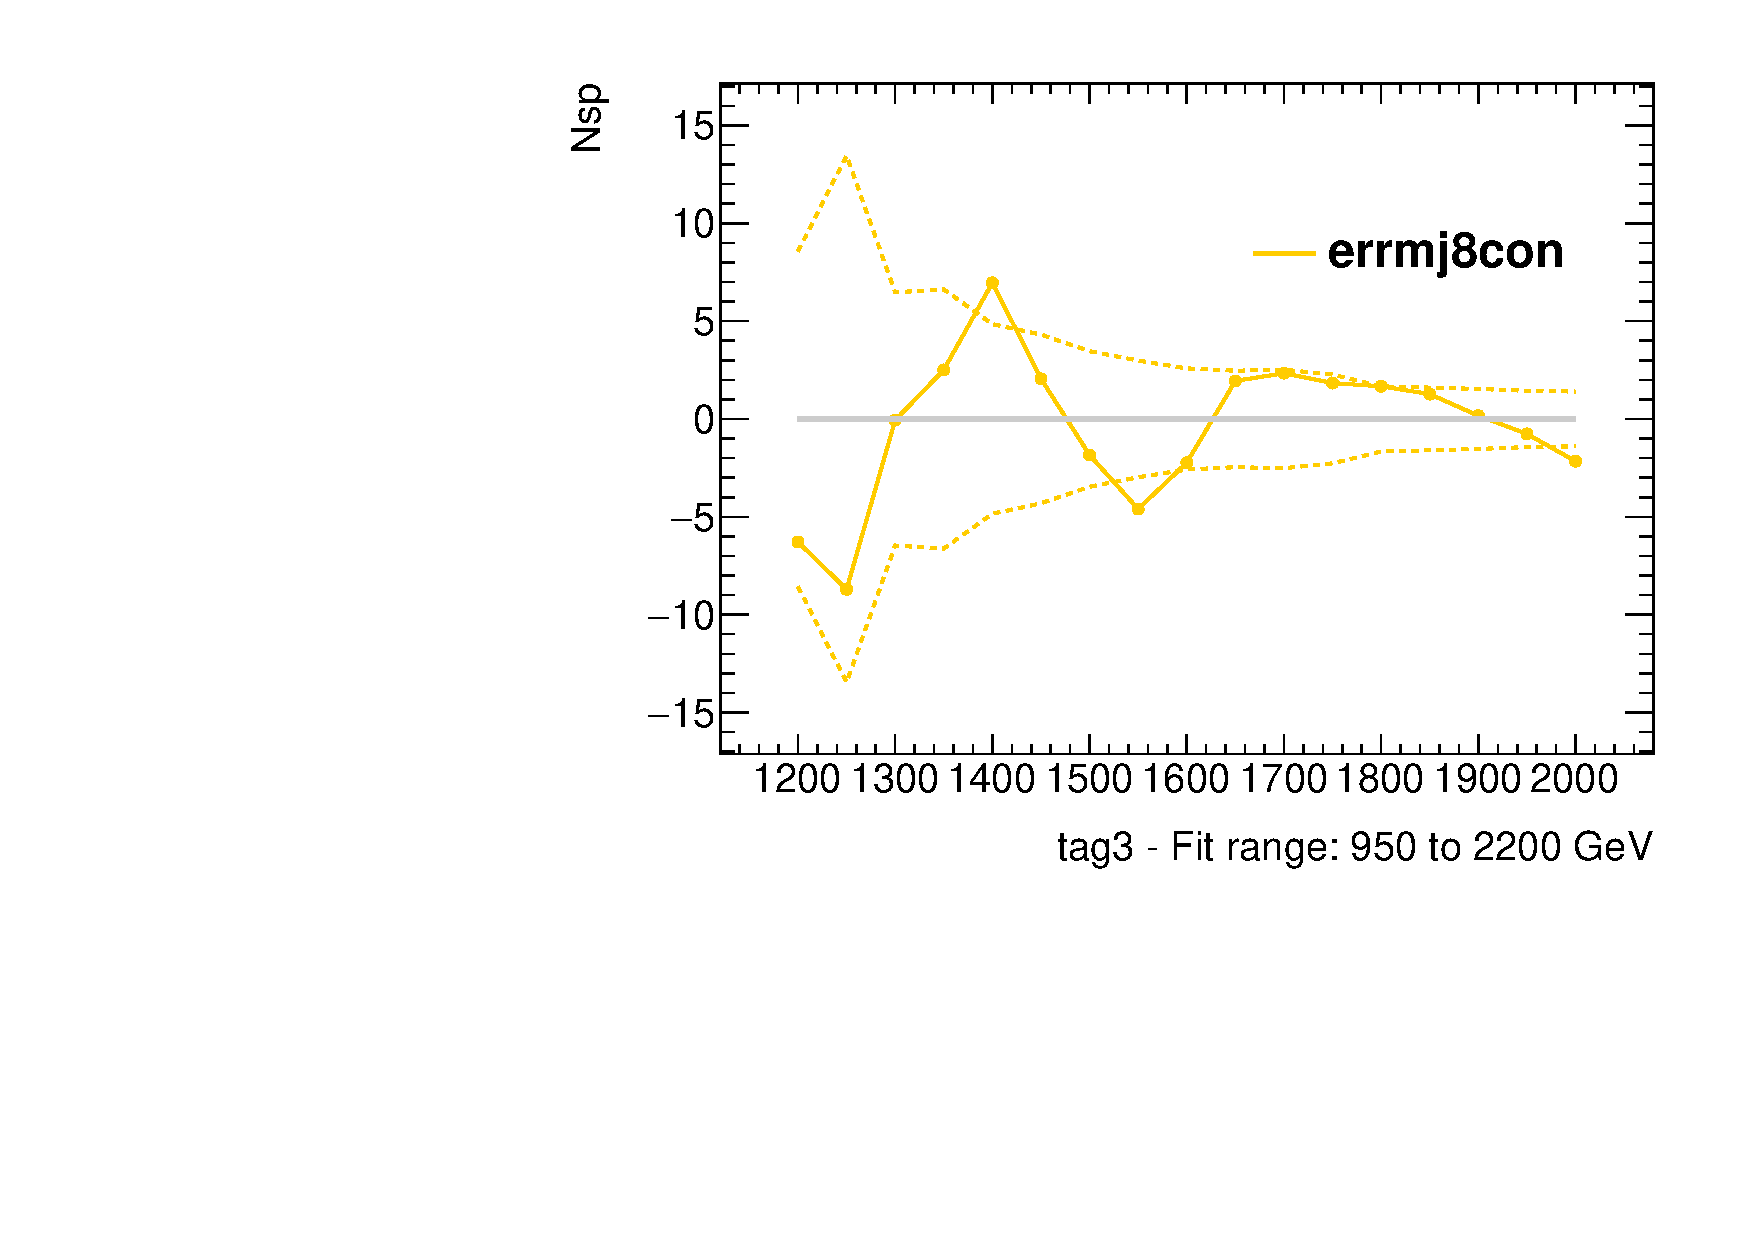
\includegraphics[angle=270, width=0.32\textwidth]{./figures/boosted/app-directfit/Nsp_tag3_range950to2200.pdf} }
\subfloat[]{ 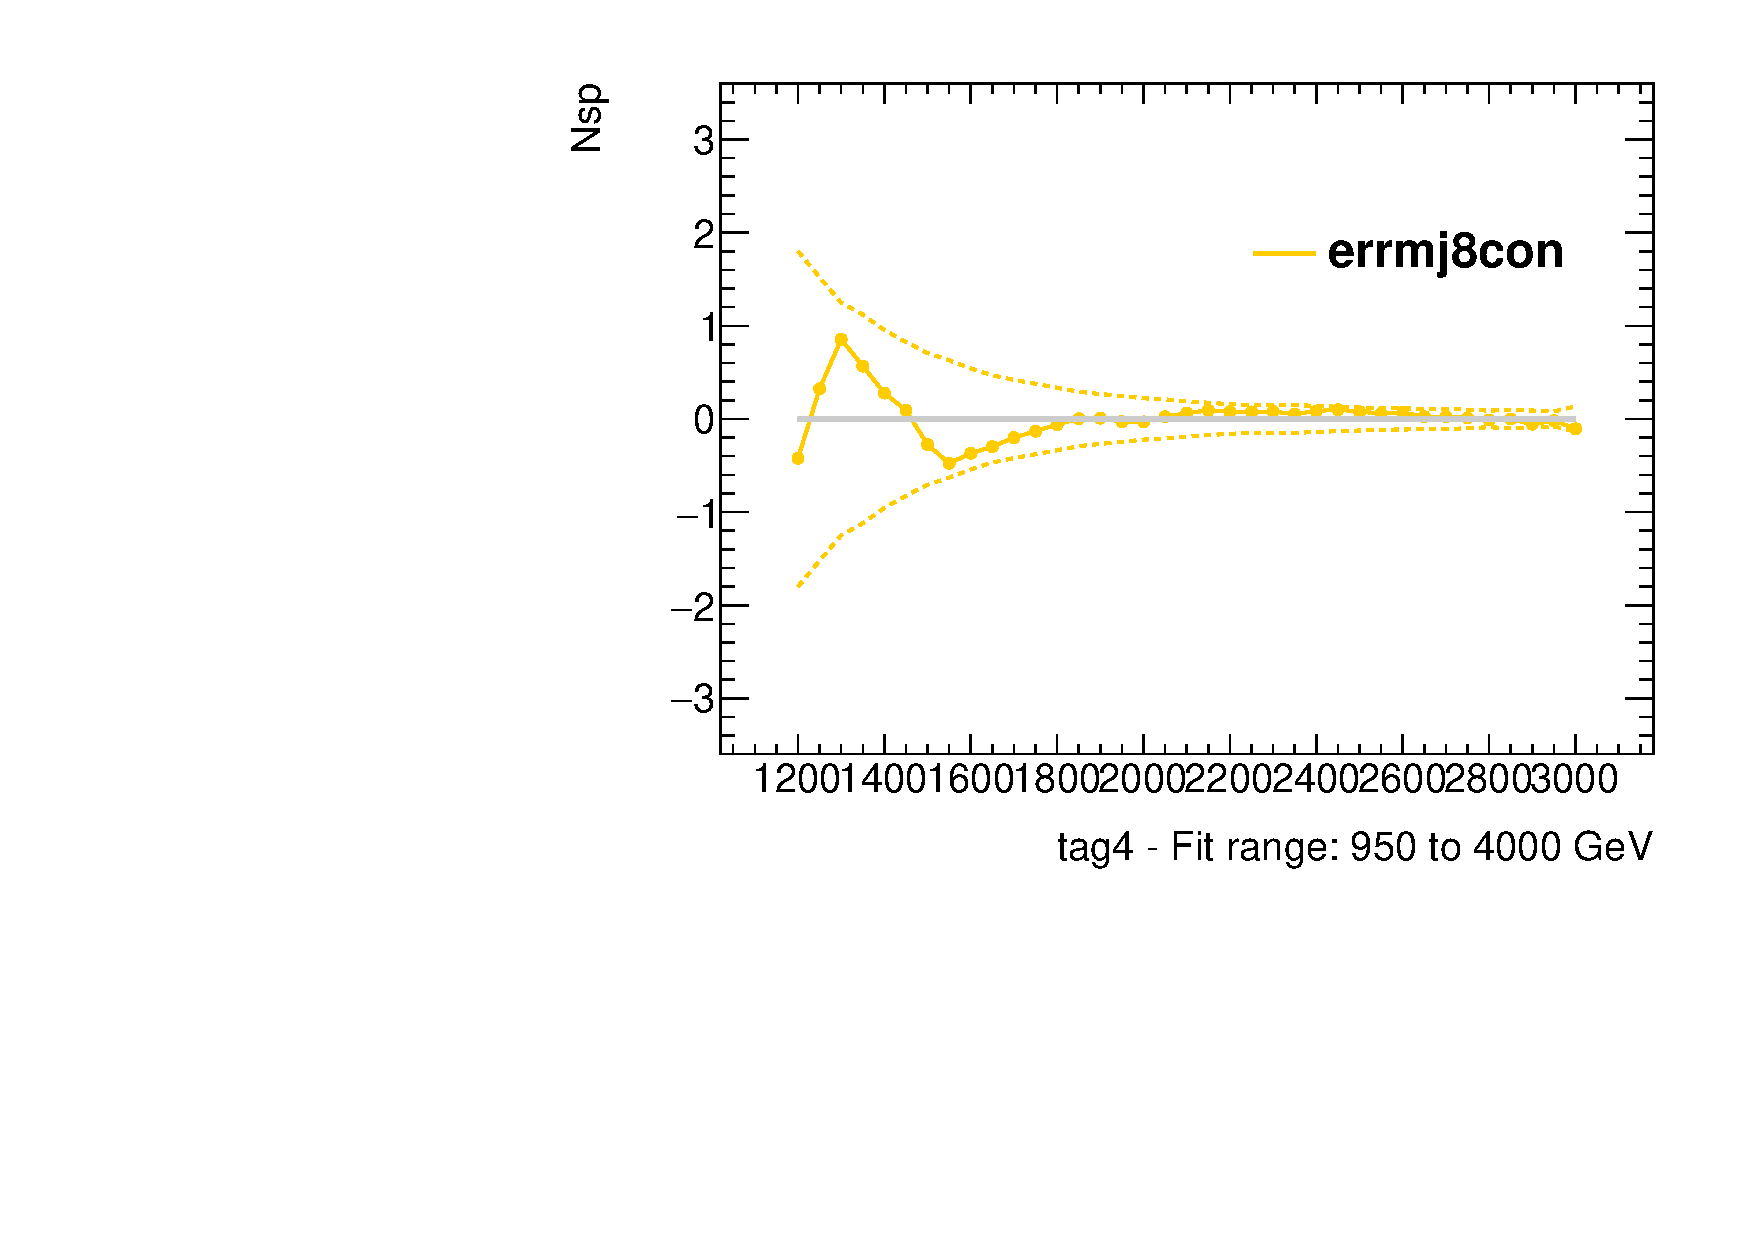
\includegraphics[angle=270, width=0.32\textwidth]{./figures/boosted/app-directfit/Nsp_tag4_range950to4000.pdf} } \\
\subfloat[]{ 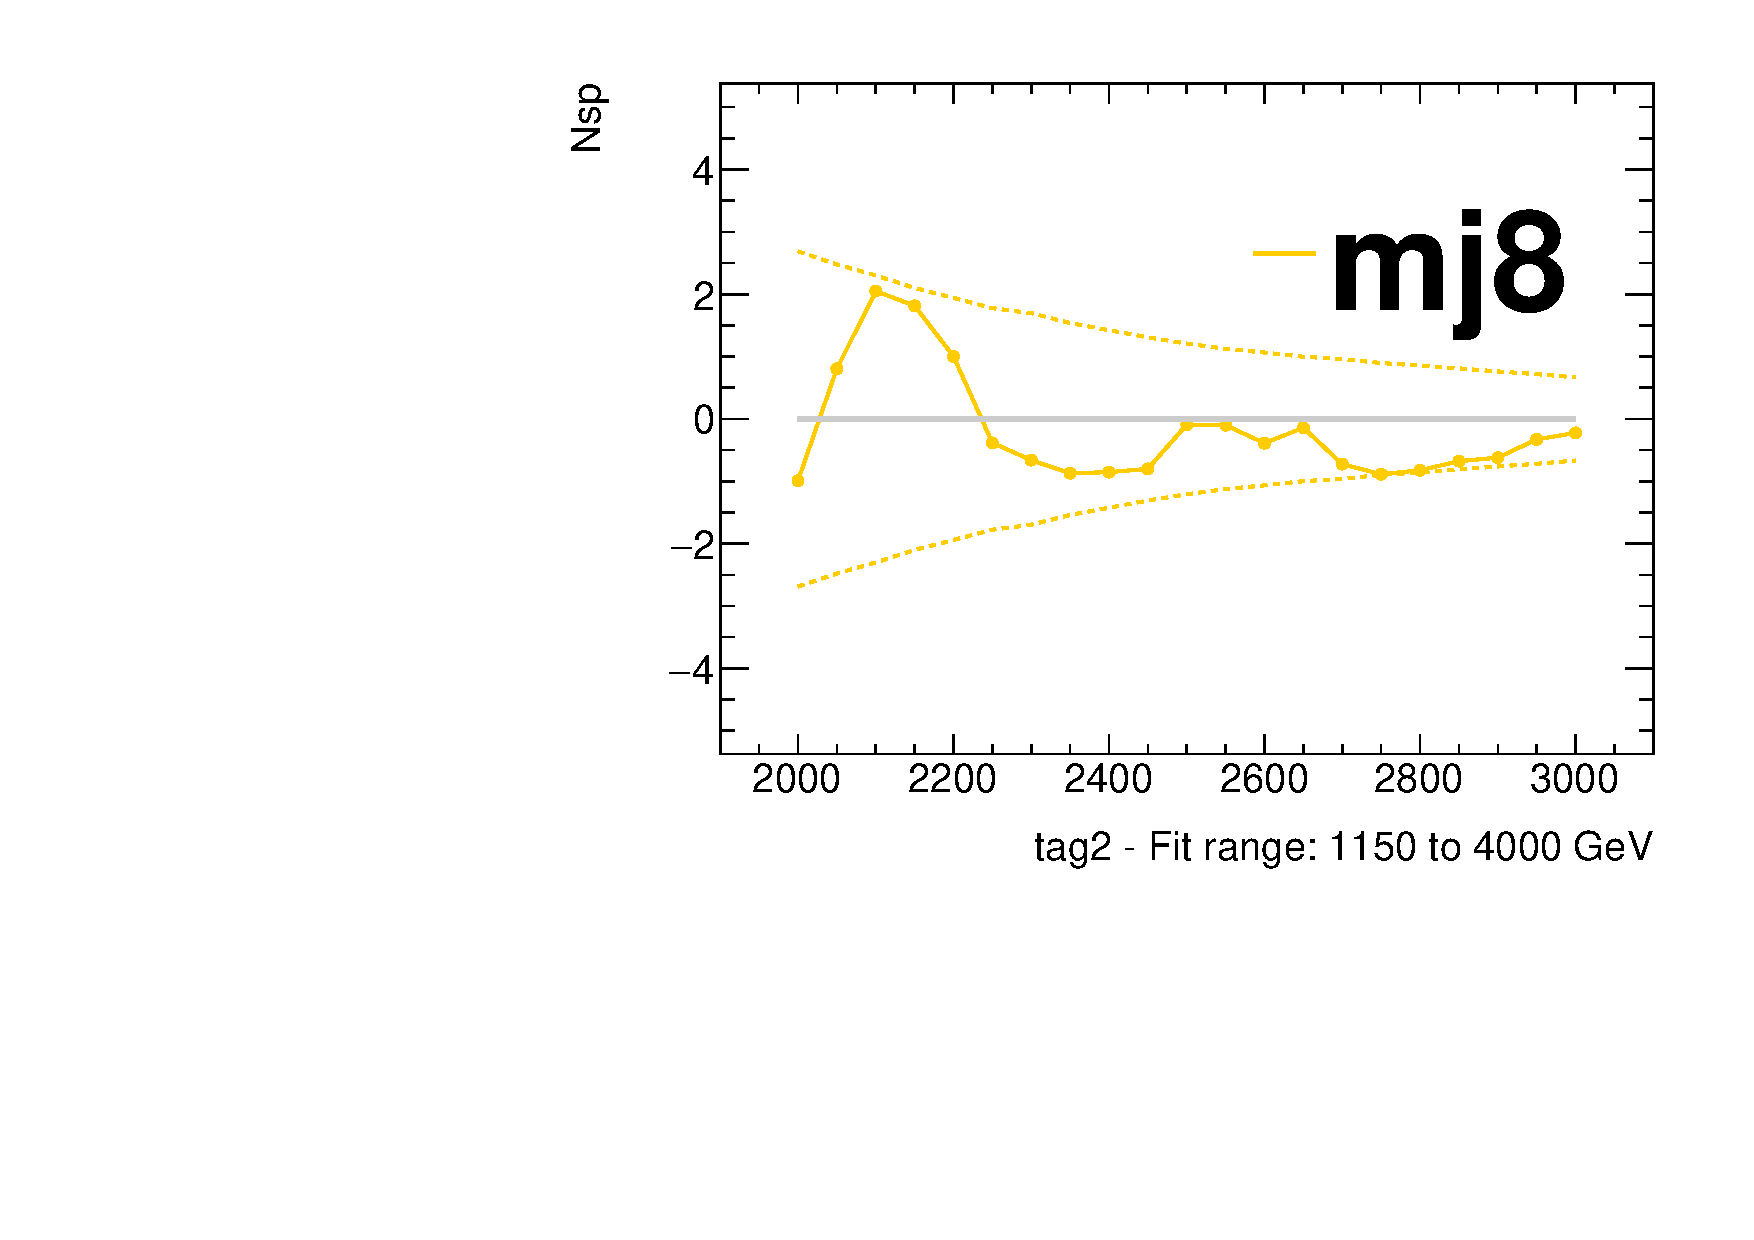
\includegraphics[angle=270, width=0.32\textwidth]{./figures/boosted/app-directfit/Nsp_tag2_range1150to4000.pdf} }
\subfloat[]{ 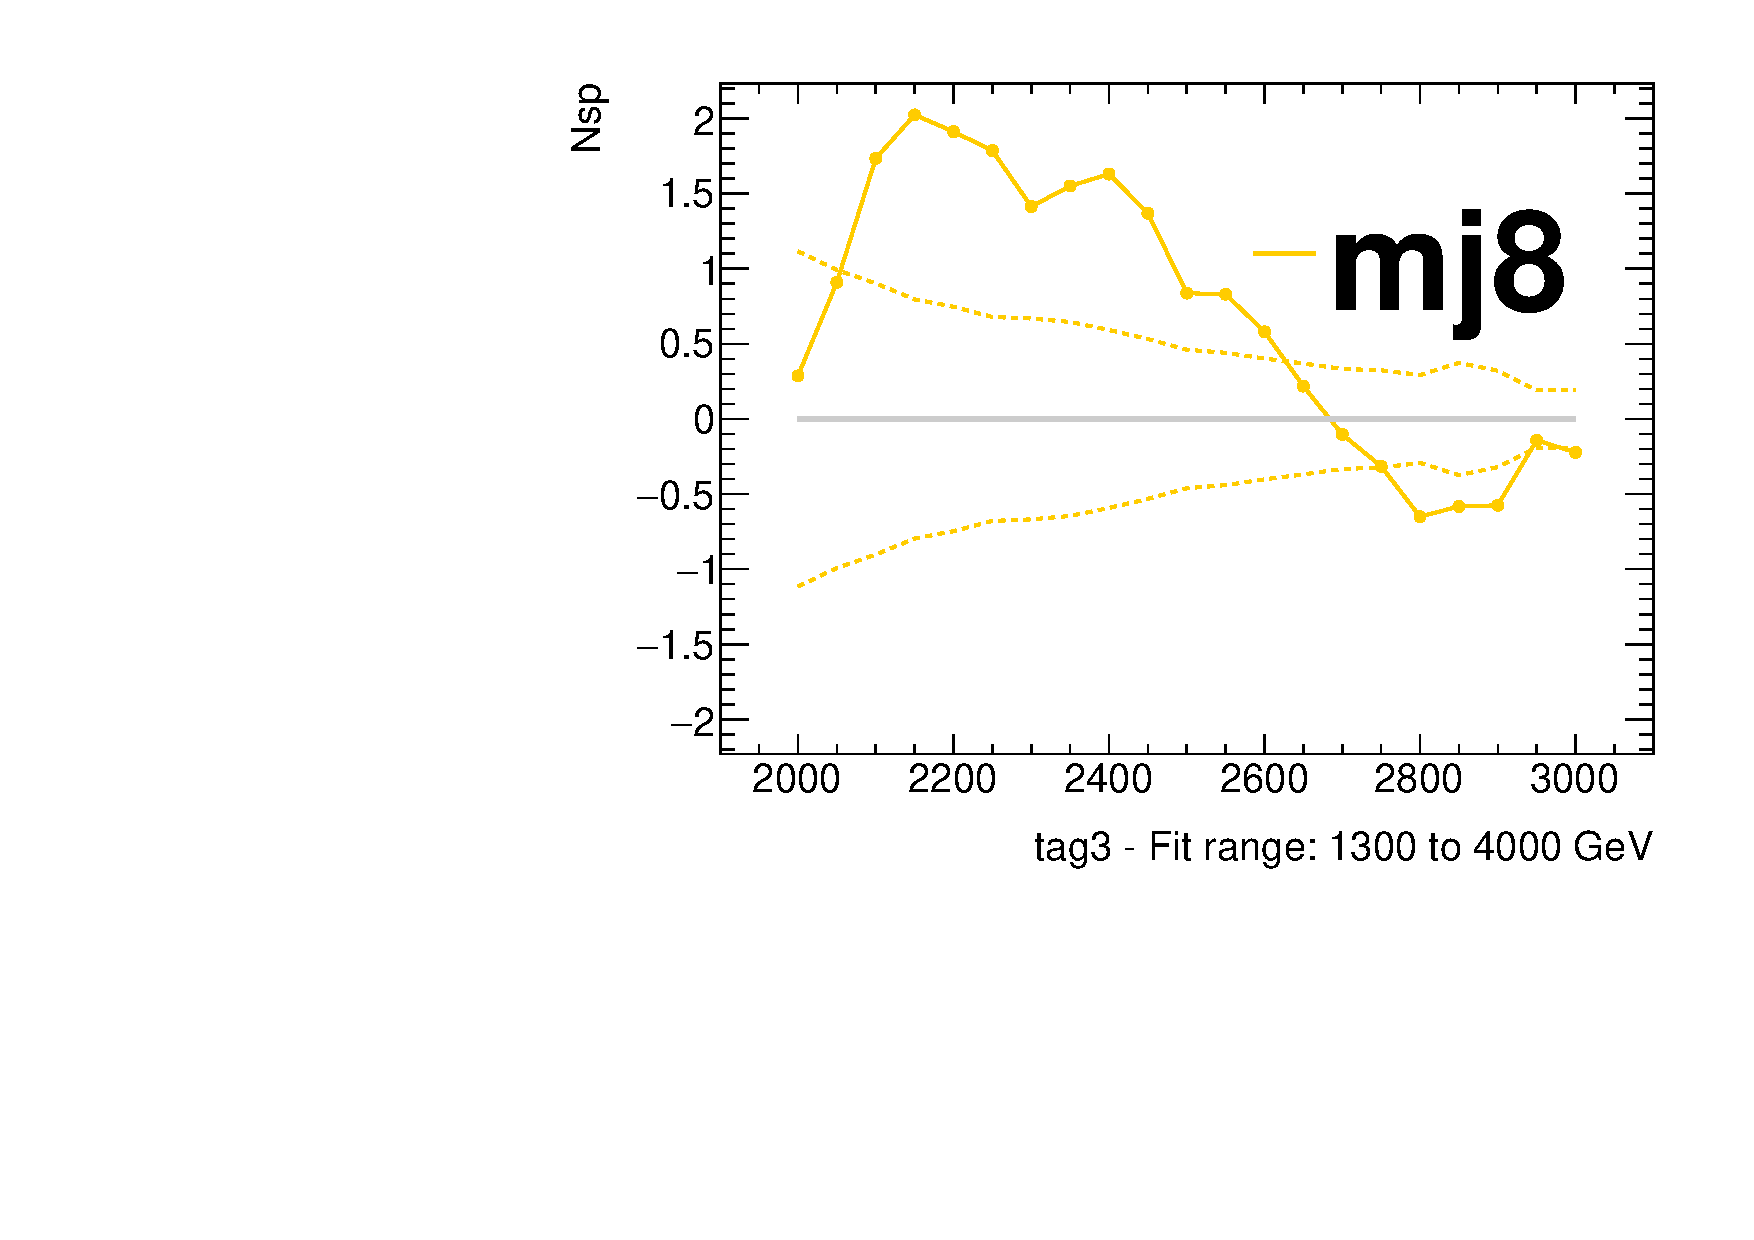
\includegraphics[angle=270, width=0.32\textwidth]{./figures/boosted/app-directfit/Nsp_tag3_range1300to4000.pdf} }
\caption{The spurious signal result, the best that was found given the variations of functions and range. The categories are: (a) 2bs low mass, (b) 3b low mass, (c) 4b, (d) 2bs high mass and (e) 3b high mass. The dashed lines indicate 20\% of the fitted signal uncertainty. The criteria is not strictly full filled in all cases.}
\label{fig:directfit:nspurious}
\end{center}
\end{figure*}

\begin{figure*}[htbp!]
\begin{center}
\subfloat[]{ 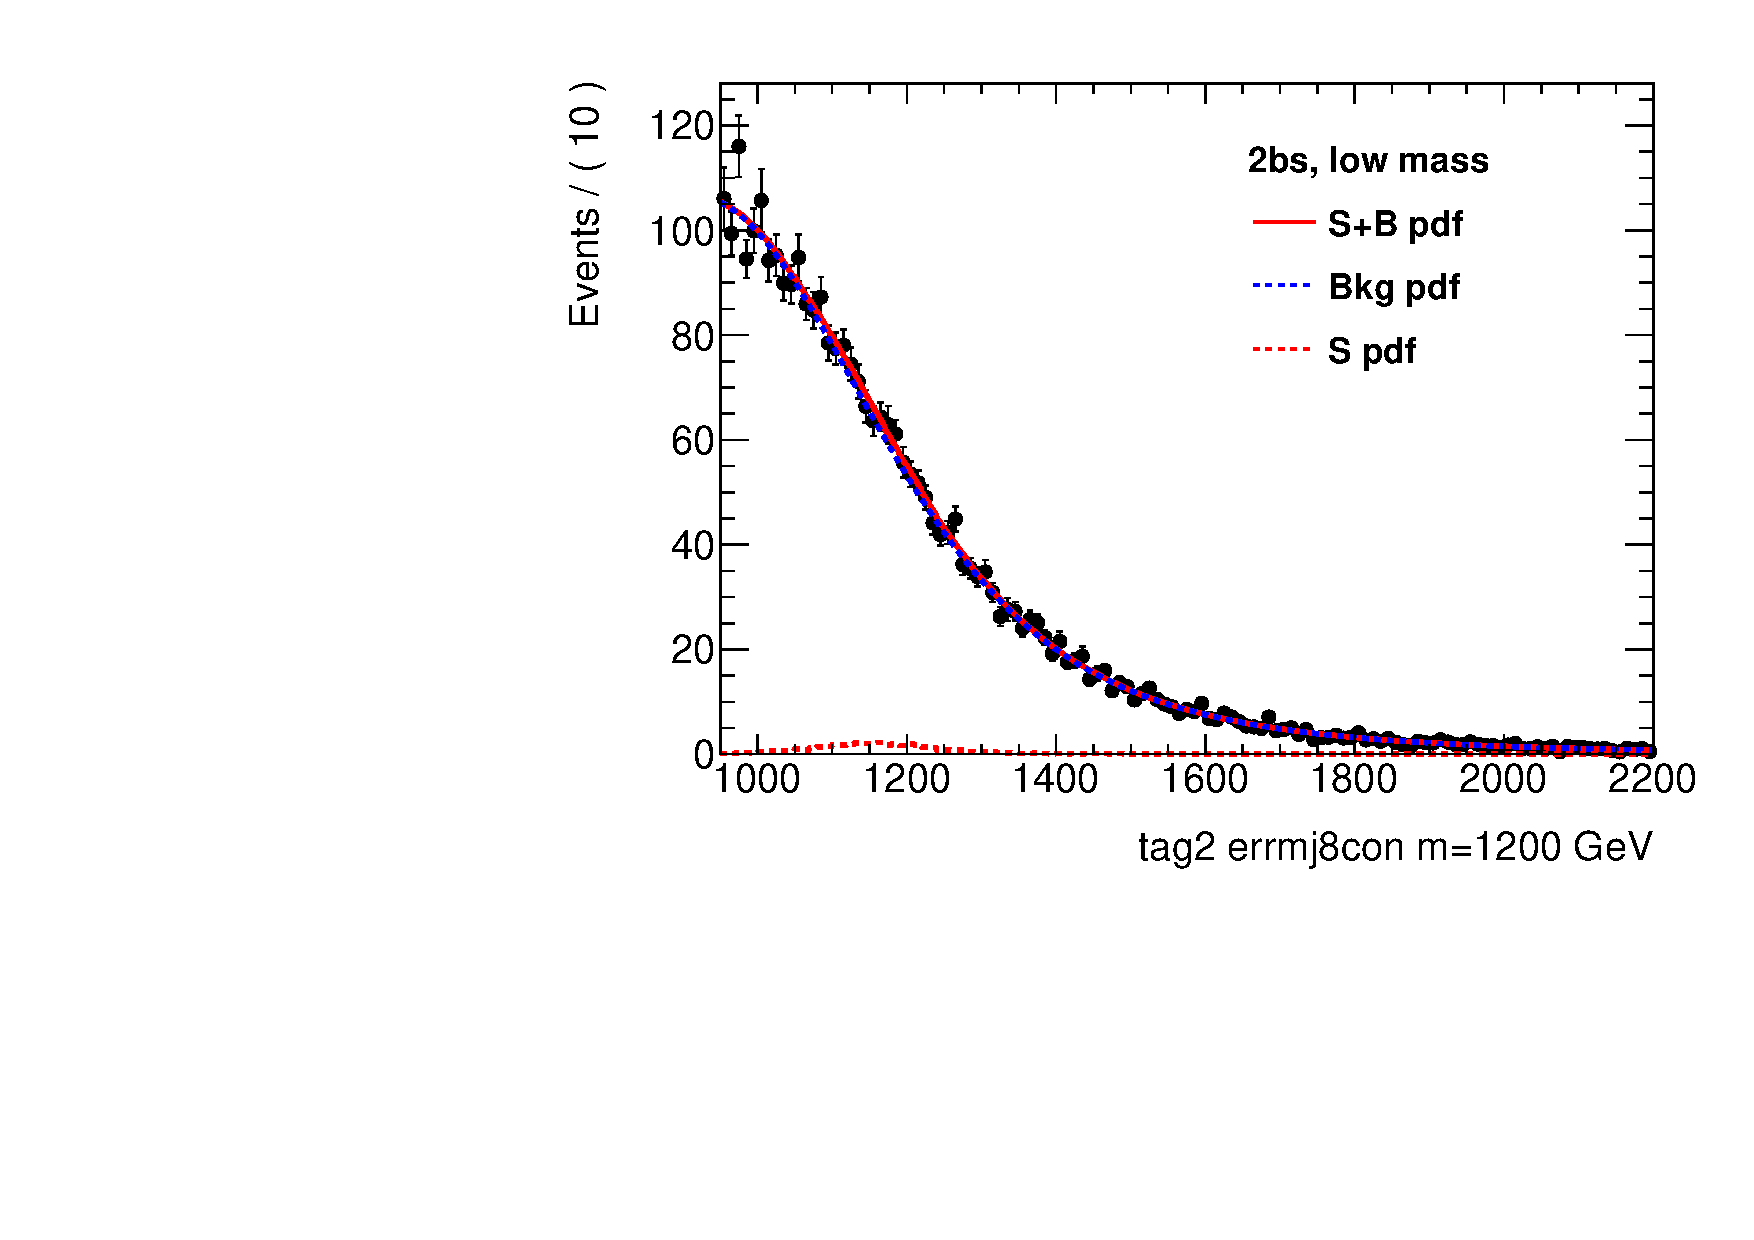
\includegraphics[angle=270, width=0.32\textwidth]{./figures/boosted/app-directfit/tag2_errmj8con_mass1200_range950to2200.pdf} }
\subfloat[]{ 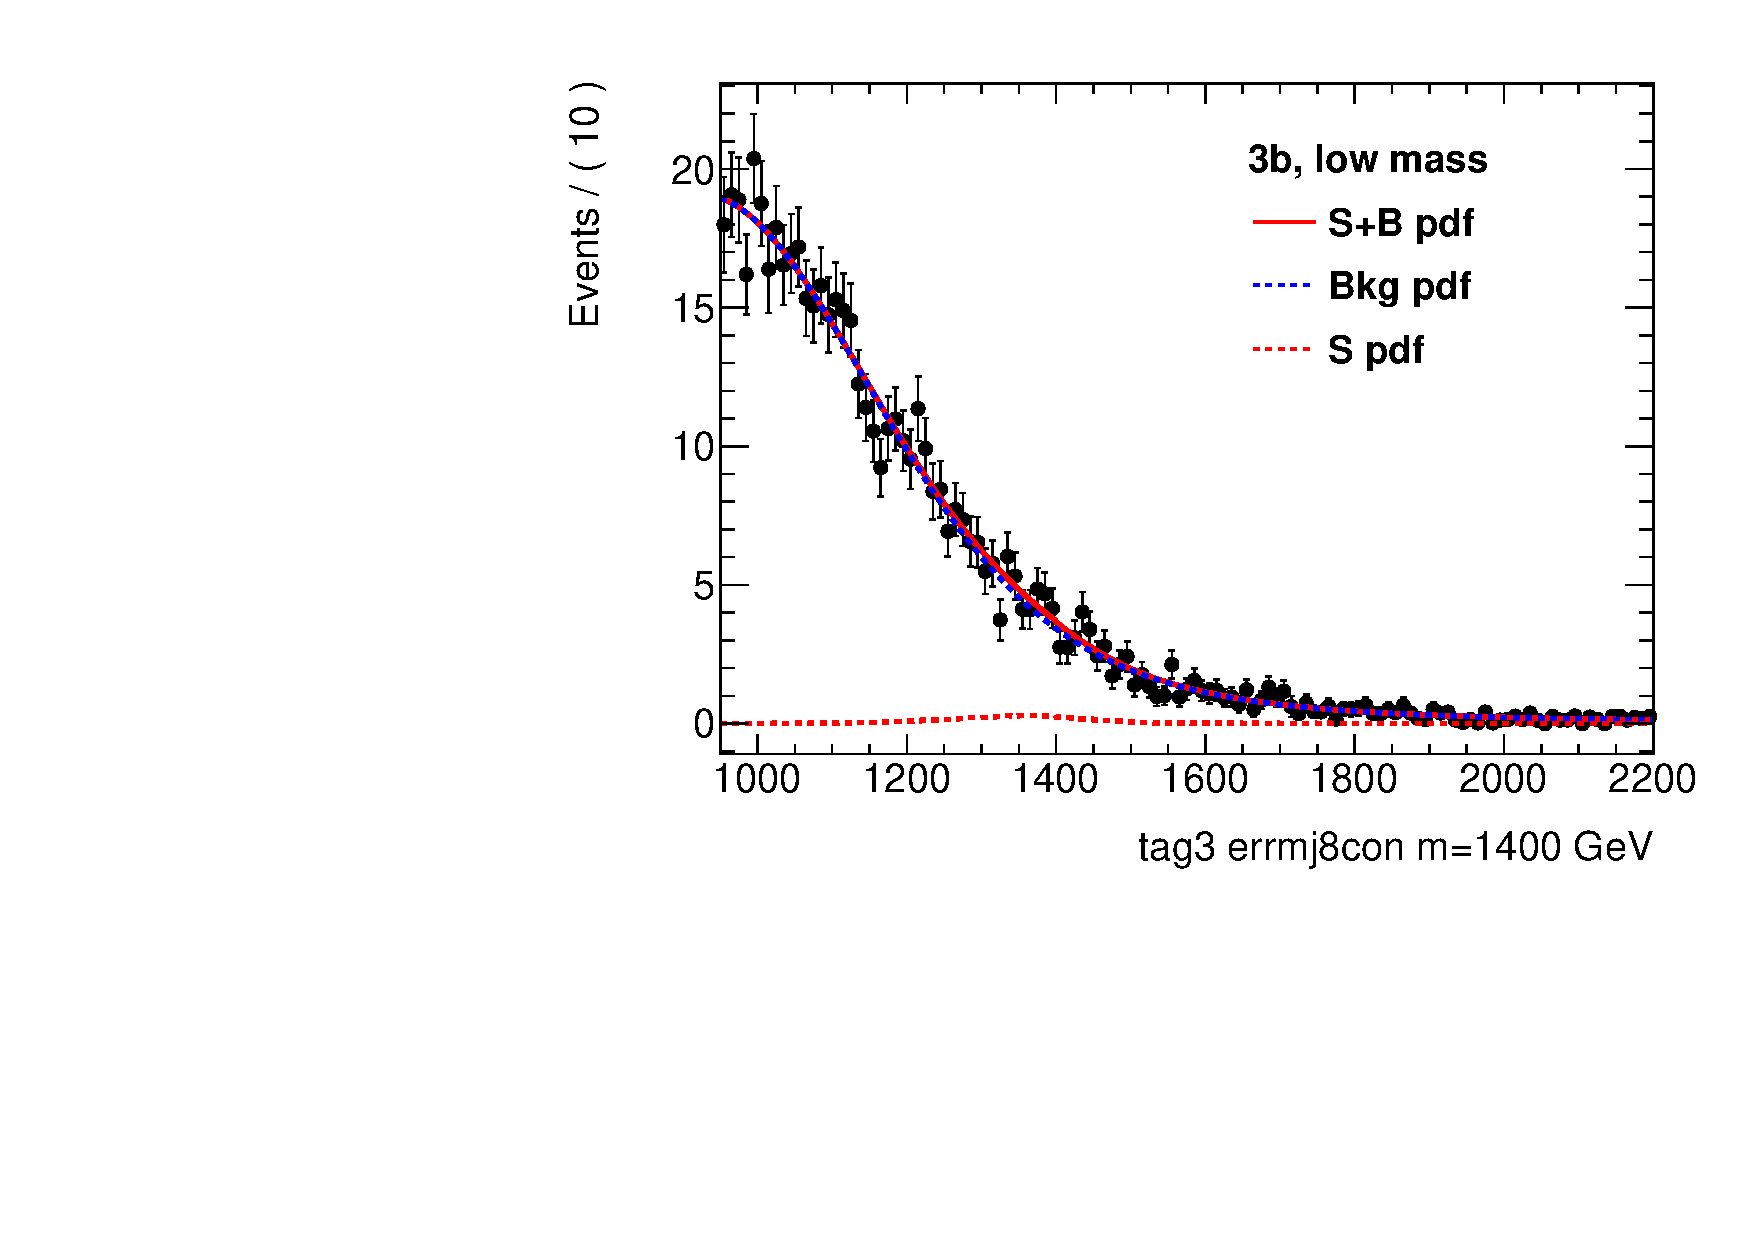
\includegraphics[angle=270, width=0.32\textwidth]{./figures/boosted/app-directfit/tag3_errmj8con_mass1400_range950to2200.pdf} }
\subfloat[]{ 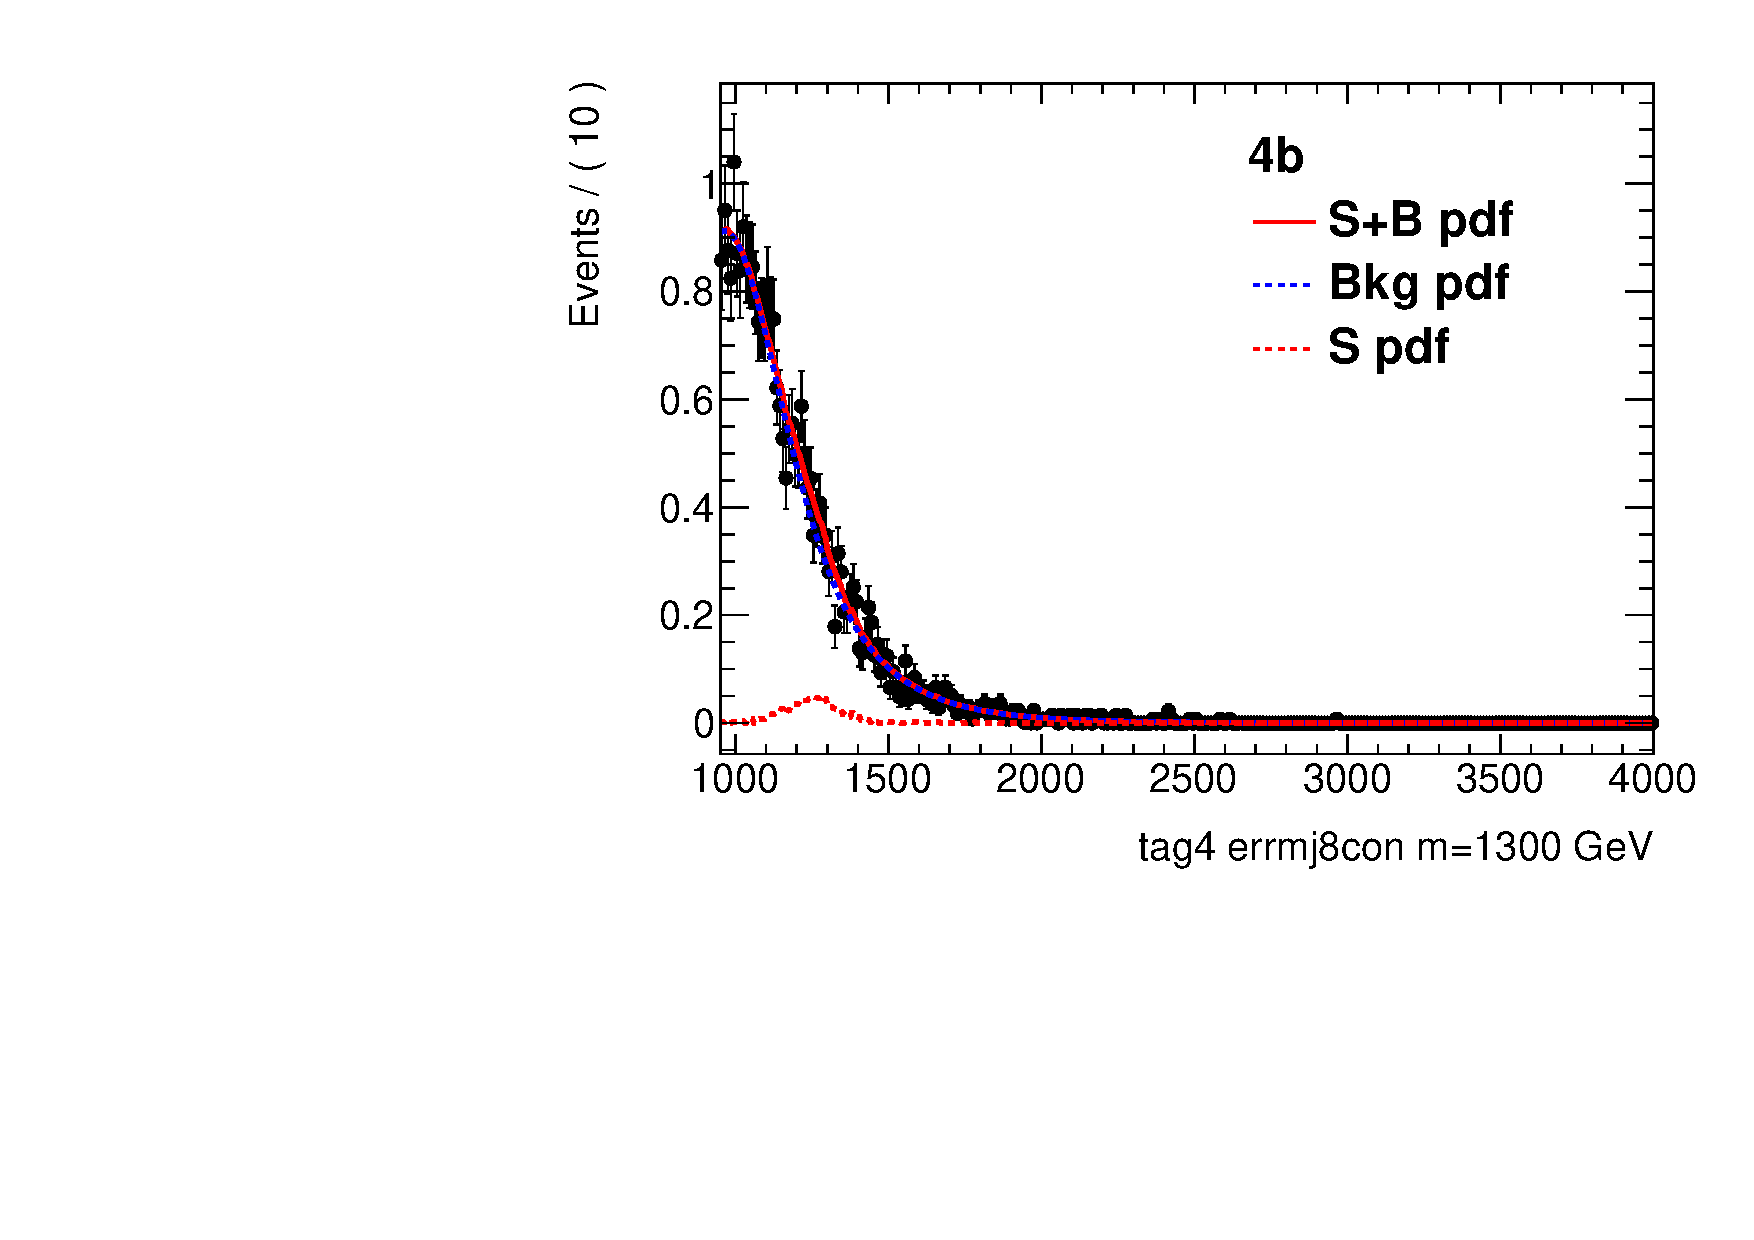
\includegraphics[angle=270, width=0.32\textwidth]{./figures/boosted/app-directfit/tag4_errmj8con_mass1300_range950to4000.pdf} } \\
\subfloat[]{ 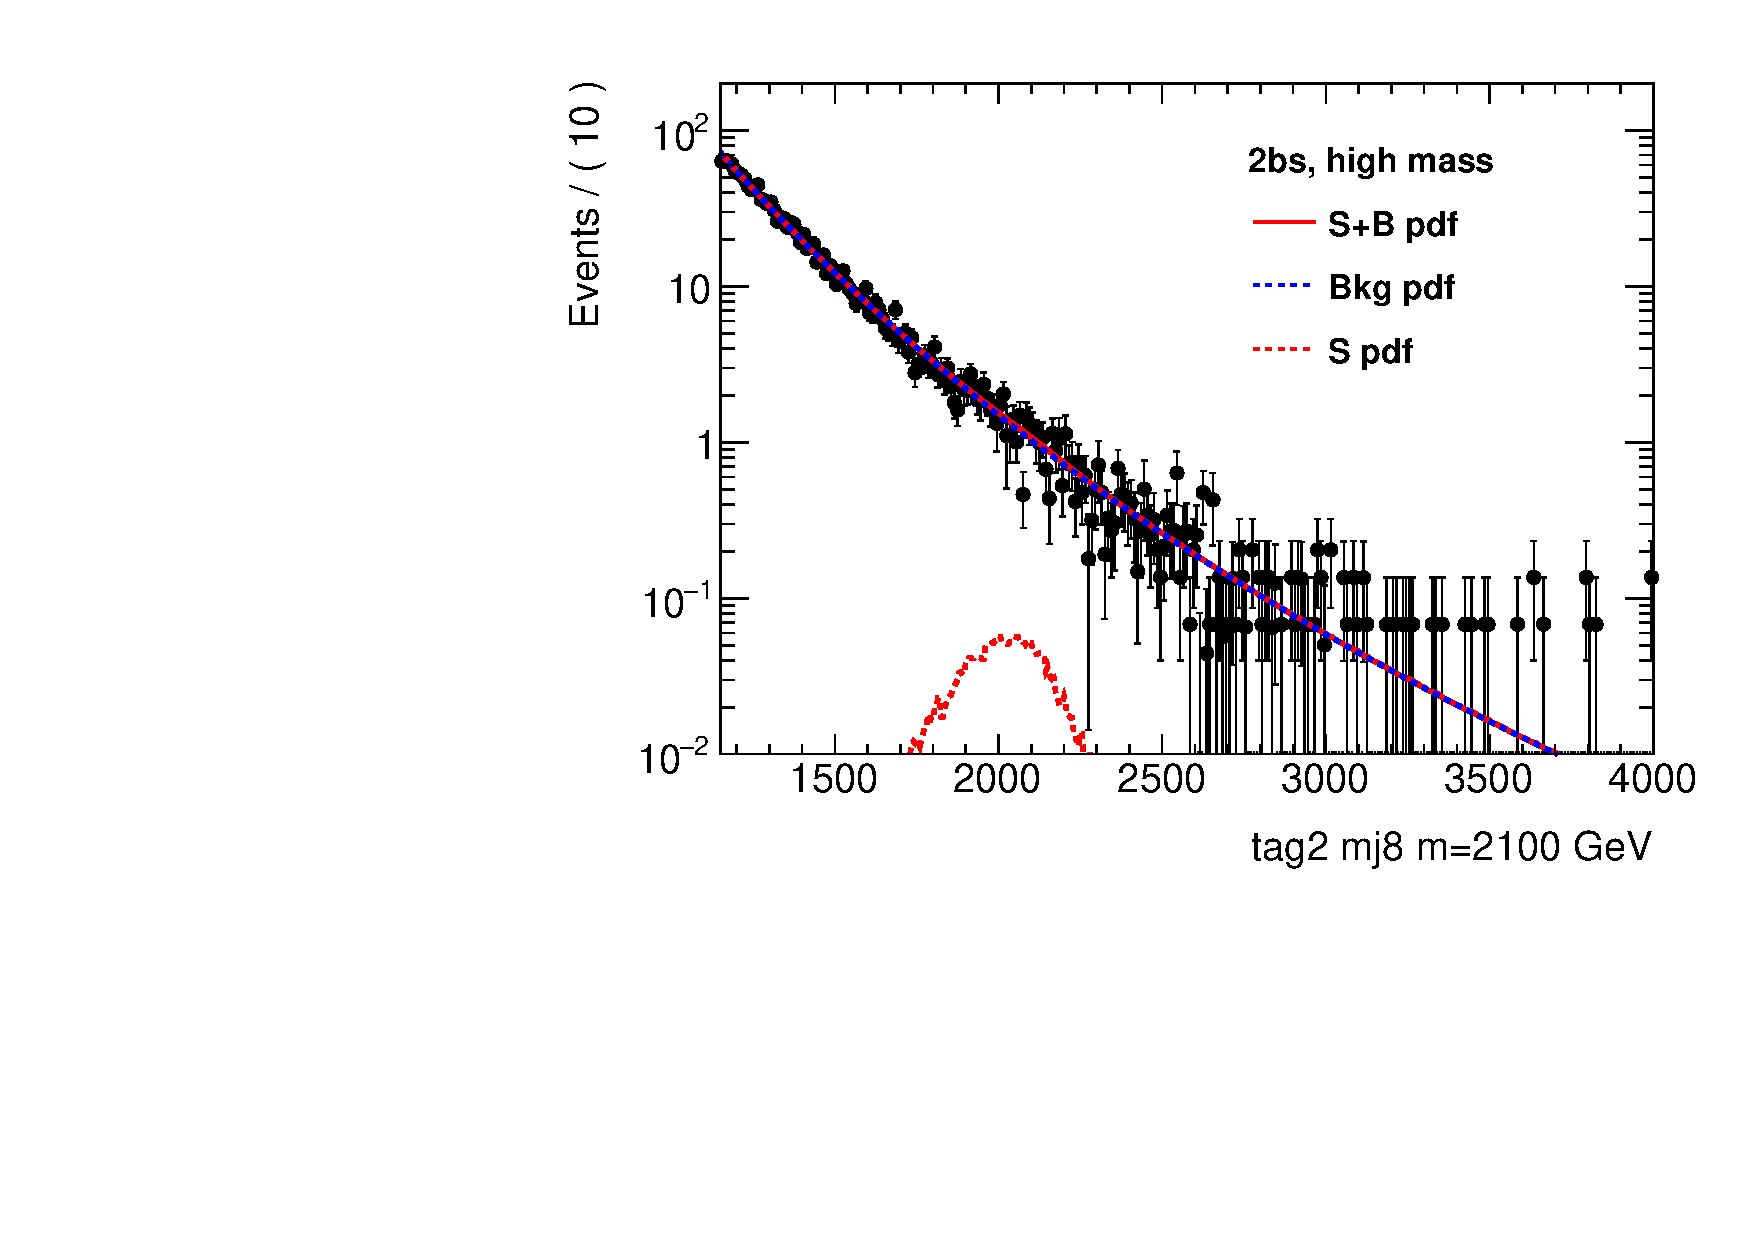
\includegraphics[angle=270, width=0.32\textwidth]{./figures/boosted/app-directfit/tag2_mj8_mass2100_range1150to4000.pdf} }
\subfloat[]{ 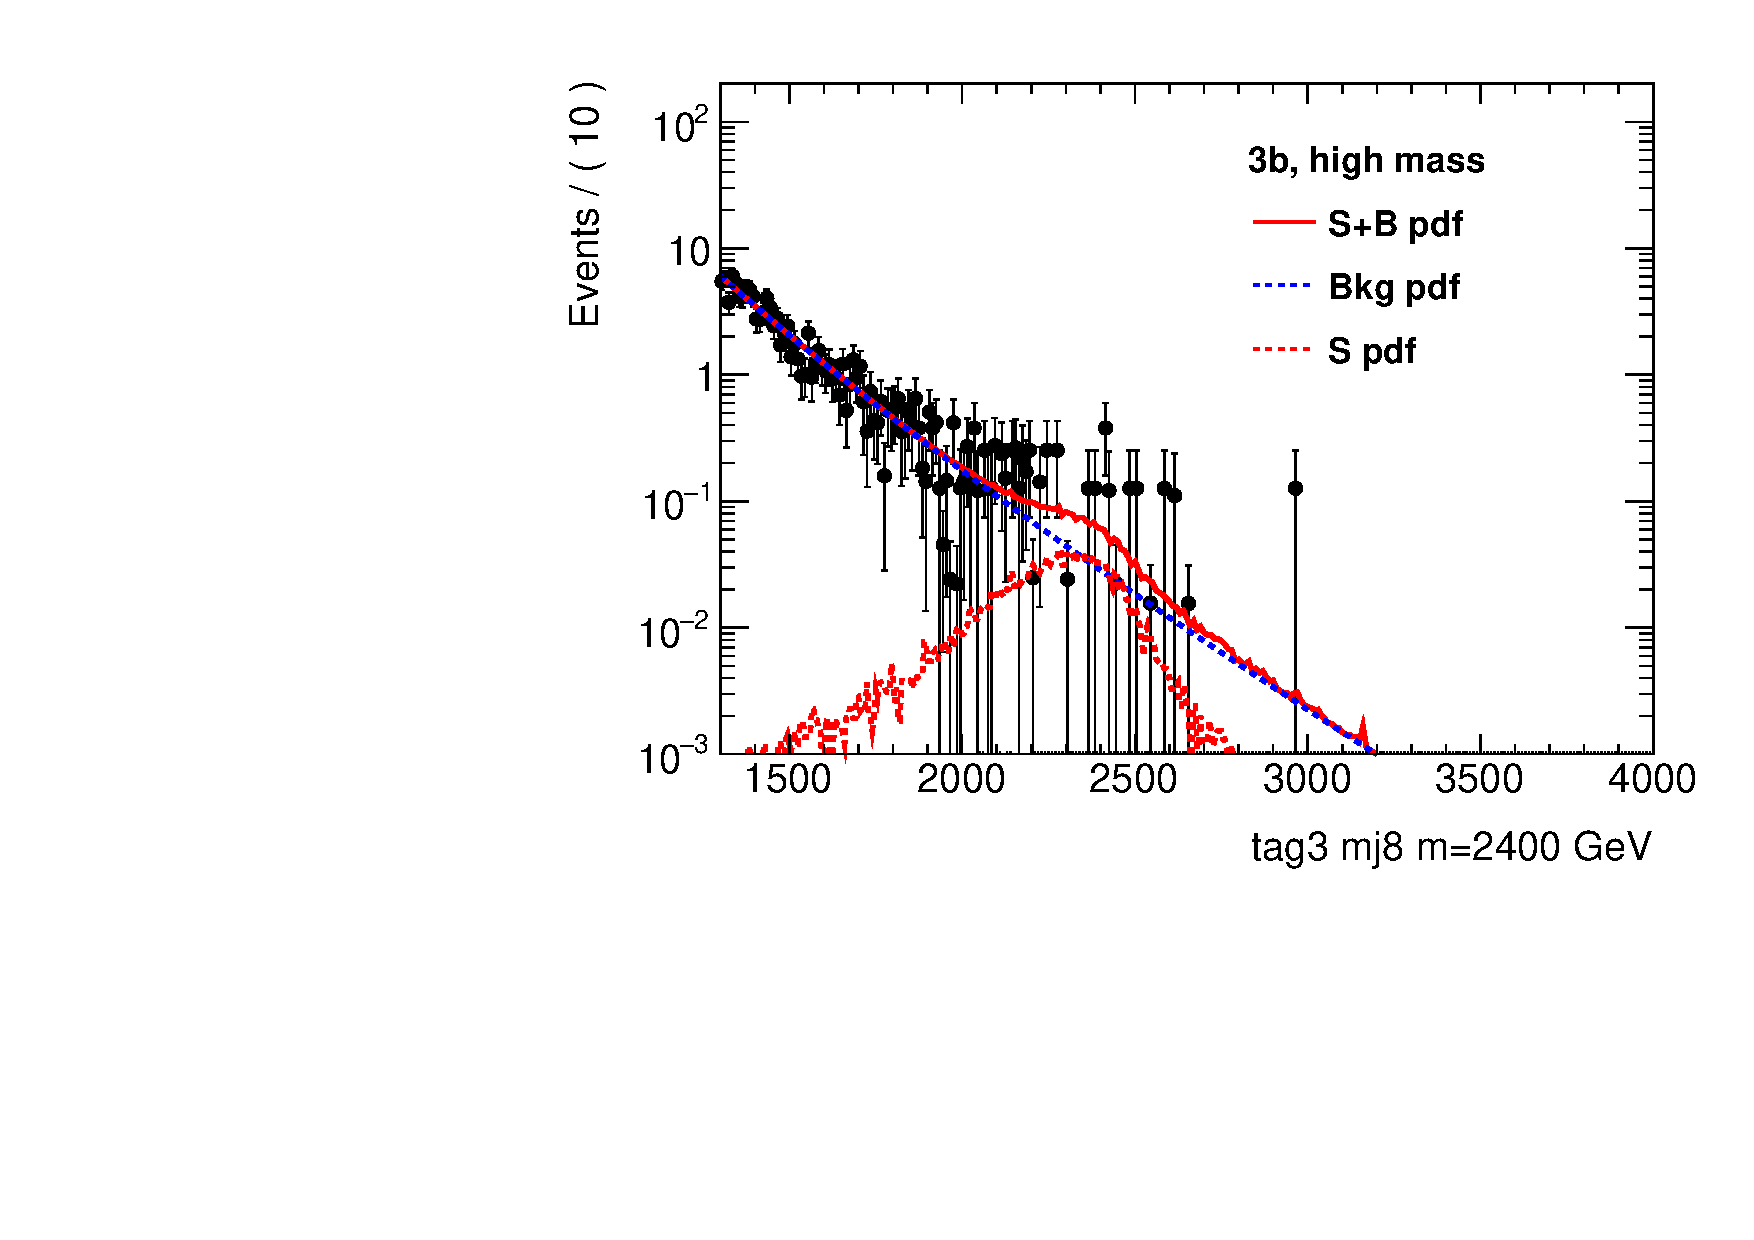
\includegraphics[angle=270, width=0.32\textwidth]{./figures/boosted/app-directfit/tag3_mj8_mass2400_range1300to4000.pdf} }
\caption{The S+B fit to the background templates, each shown for that mass point where the spurious signal is the largest. The categories are: (a) 2bs low mass, (b) 3b low mass, (c) 4b, (d) 2bs high mass and (e) 3b high mass.}
\label{fig:directfit:splubfitplots}
\end{center}
\end{figure*}

It is clear from this study, that the spurious signal is not negligible sometimes. Though the dijet functions work the best, it seems that they are not doing a perfect job in the modelling. In the future, with more luminosity, it might be worth investigating other functions, or function-less fits (such as Gaussian processes).

\subsection{Eigenvector variations}

Since the signal is modelled through histogram templates, the background also needs to be converted to histograms. Then, HistFactory can be used to build workspace and do the statistical analysis.
But with the histogram-based approach, the background is essentially fixed in a given template. But the nuisance from the parameters describing the functional form (eg. the two parameters from the turn-on, and the two parameters from the MJ8 function) needs to be incorporated in order to do the actual fit. The idea here is to retrieve eigenvector variations from the covariance matrix after the background-only fit. Eigenvectors are orthogonal to each other, and they point to the direction of the largest variance. The technical procedure is:

\begin{itemize}
\item Do background-only fit to the background-templates (or to the pseudo-data, or real data) and extract covariance matrix
\item Obtain the eigenvectors U and eigenvalues S from the covariance matrix
\item Calculate the standard deviation from the eigenvalues $\sigma=\sqrt{S}$
\item Get the "variation vectors" V from $V=U\cdot \vec{\sigma}$, with eg. $\vec{\sigma}=(\sigma_1,0)$ and $\vec{\sigma}=(0,\sigma_2)$
\item Apply these variations to the parameters of the function: $\left(p_1,p_2\right)_{vary}=\left(p_1,p_2\right)_{nominal} \pm V$, so with other words each variation will change all parameters at once, not just one
\end{itemize}

So by building histogram templates from those variations, the nuisance will be taken into account, including the correlations between the parameters. 

\subsection{Pseudo-data tests}

In order to test the fits without unblinding the data, pseudo-data is generated from the background-templates, with the same number of events as the real data. Then, many of these toy datasets are fitted, using the same procedure as would be used for the real data.

The first test is to do background-only fits. Those are needed in order to extract the eigenvector variations. In Fig.~\ref{fig:directfit:pseudobkgfits}, the background-only fits are plotted for 100 toys, simply overlayed with each other, to see the spread of those functions. As expected, the spread is smaller if a category contains more events. In the 4b category, the spread is very large.

\begin{figure*}[htbp!]
\begin{center}
\subfloat[]{ 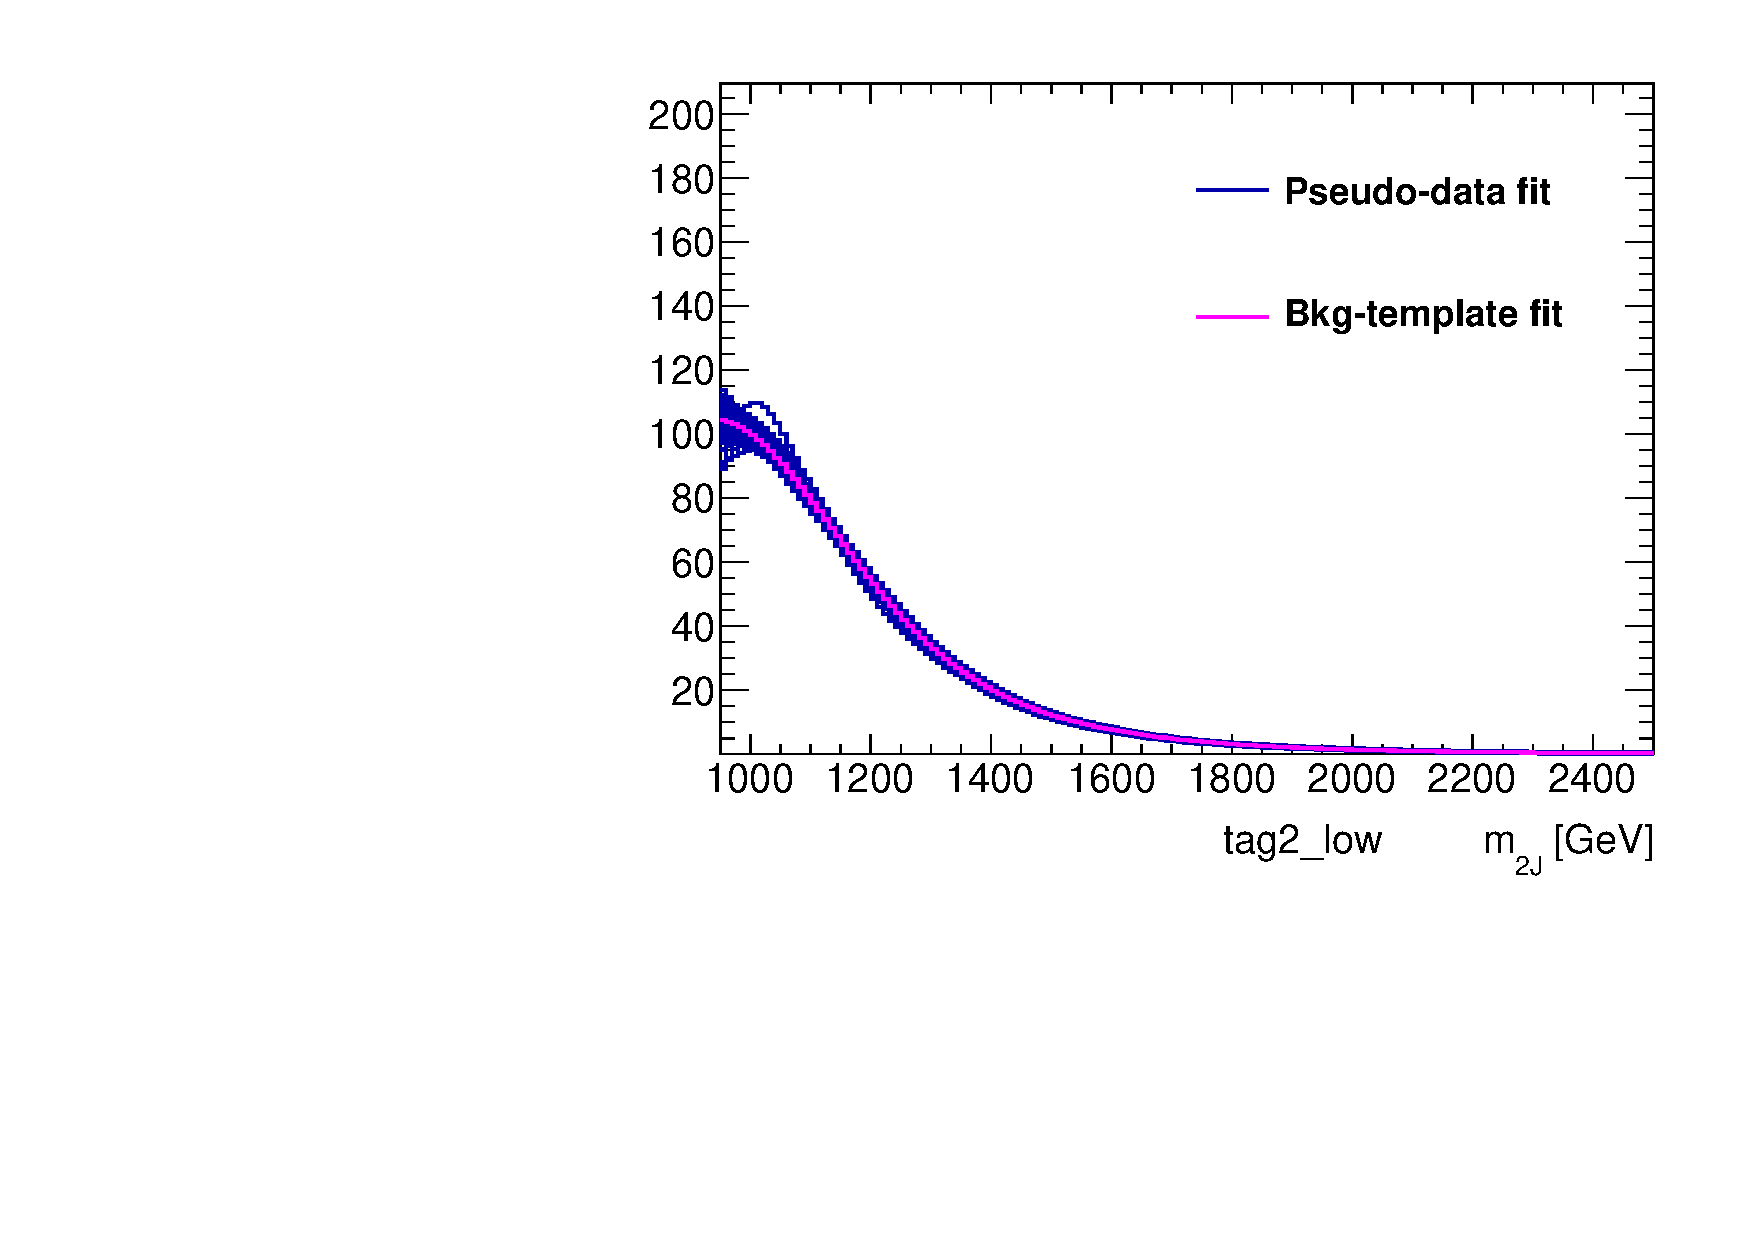
\includegraphics[angle=270, width=0.32\textwidth]{./figures/boosted/app-directfit/overlay_bonly_tag2_low.pdf} }
\subfloat[]{ 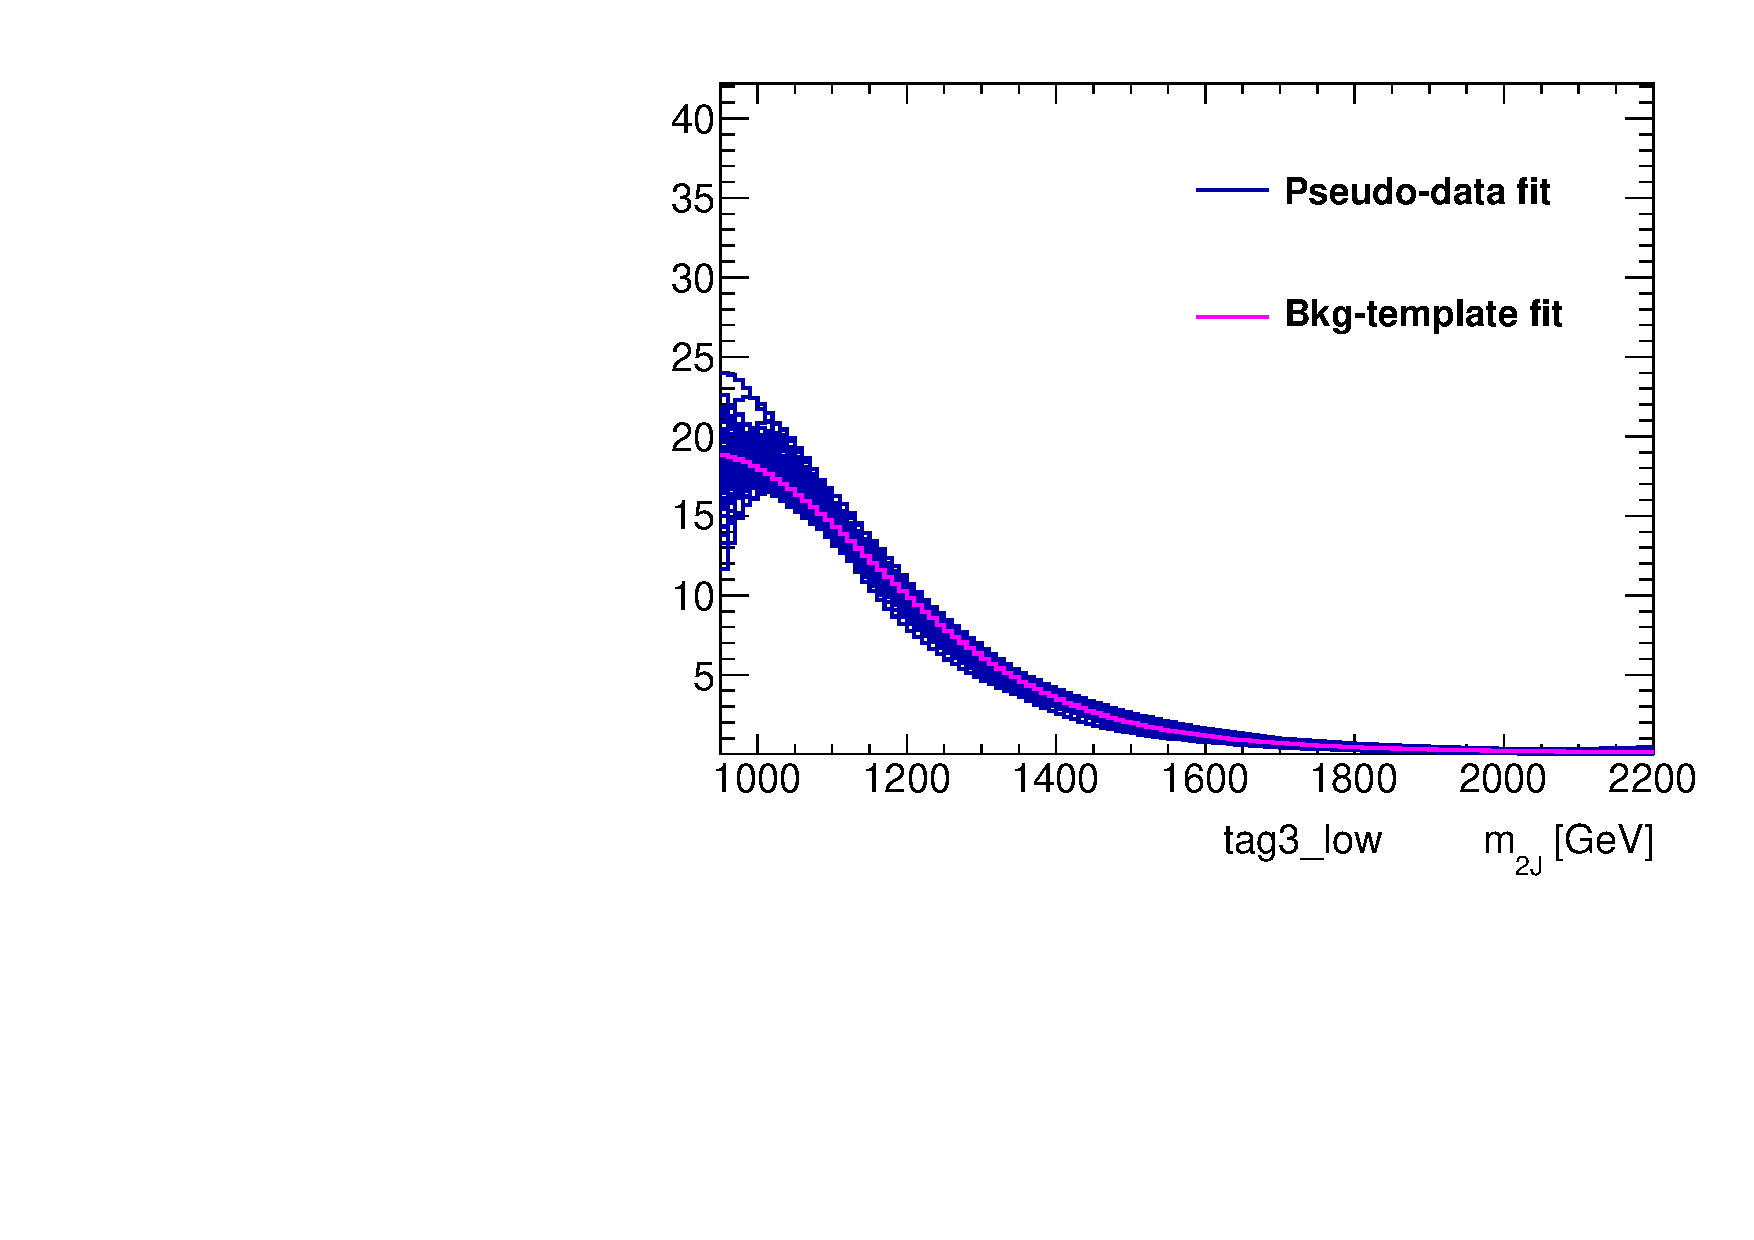
\includegraphics[angle=270, width=0.32\textwidth]{./figures/boosted/app-directfit/overlay_bonly_tag3_low.pdf} }
\subfloat[]{ 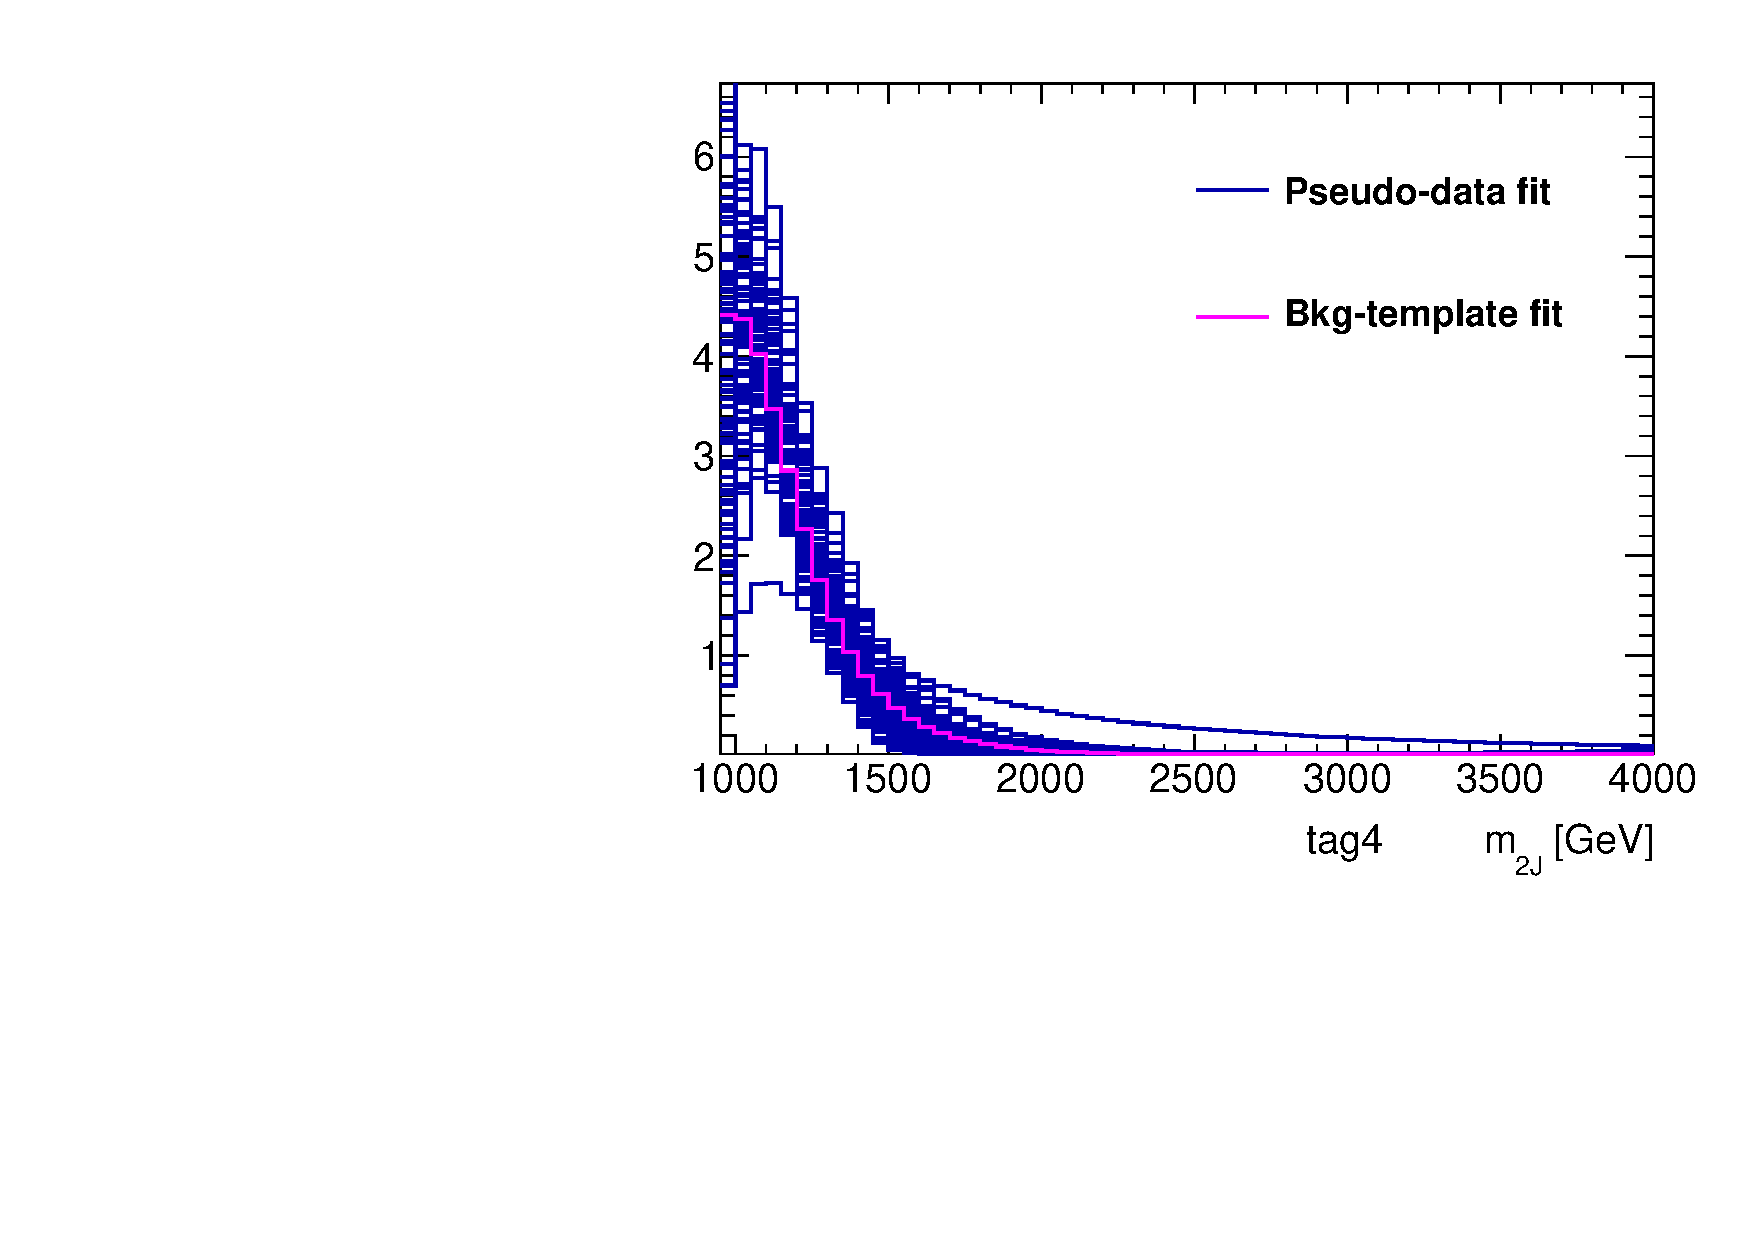
\includegraphics[angle=270, width=0.32\textwidth]{./figures/boosted/app-directfit/overlay_bonly_tag4.pdf} } \\
\subfloat[]{ 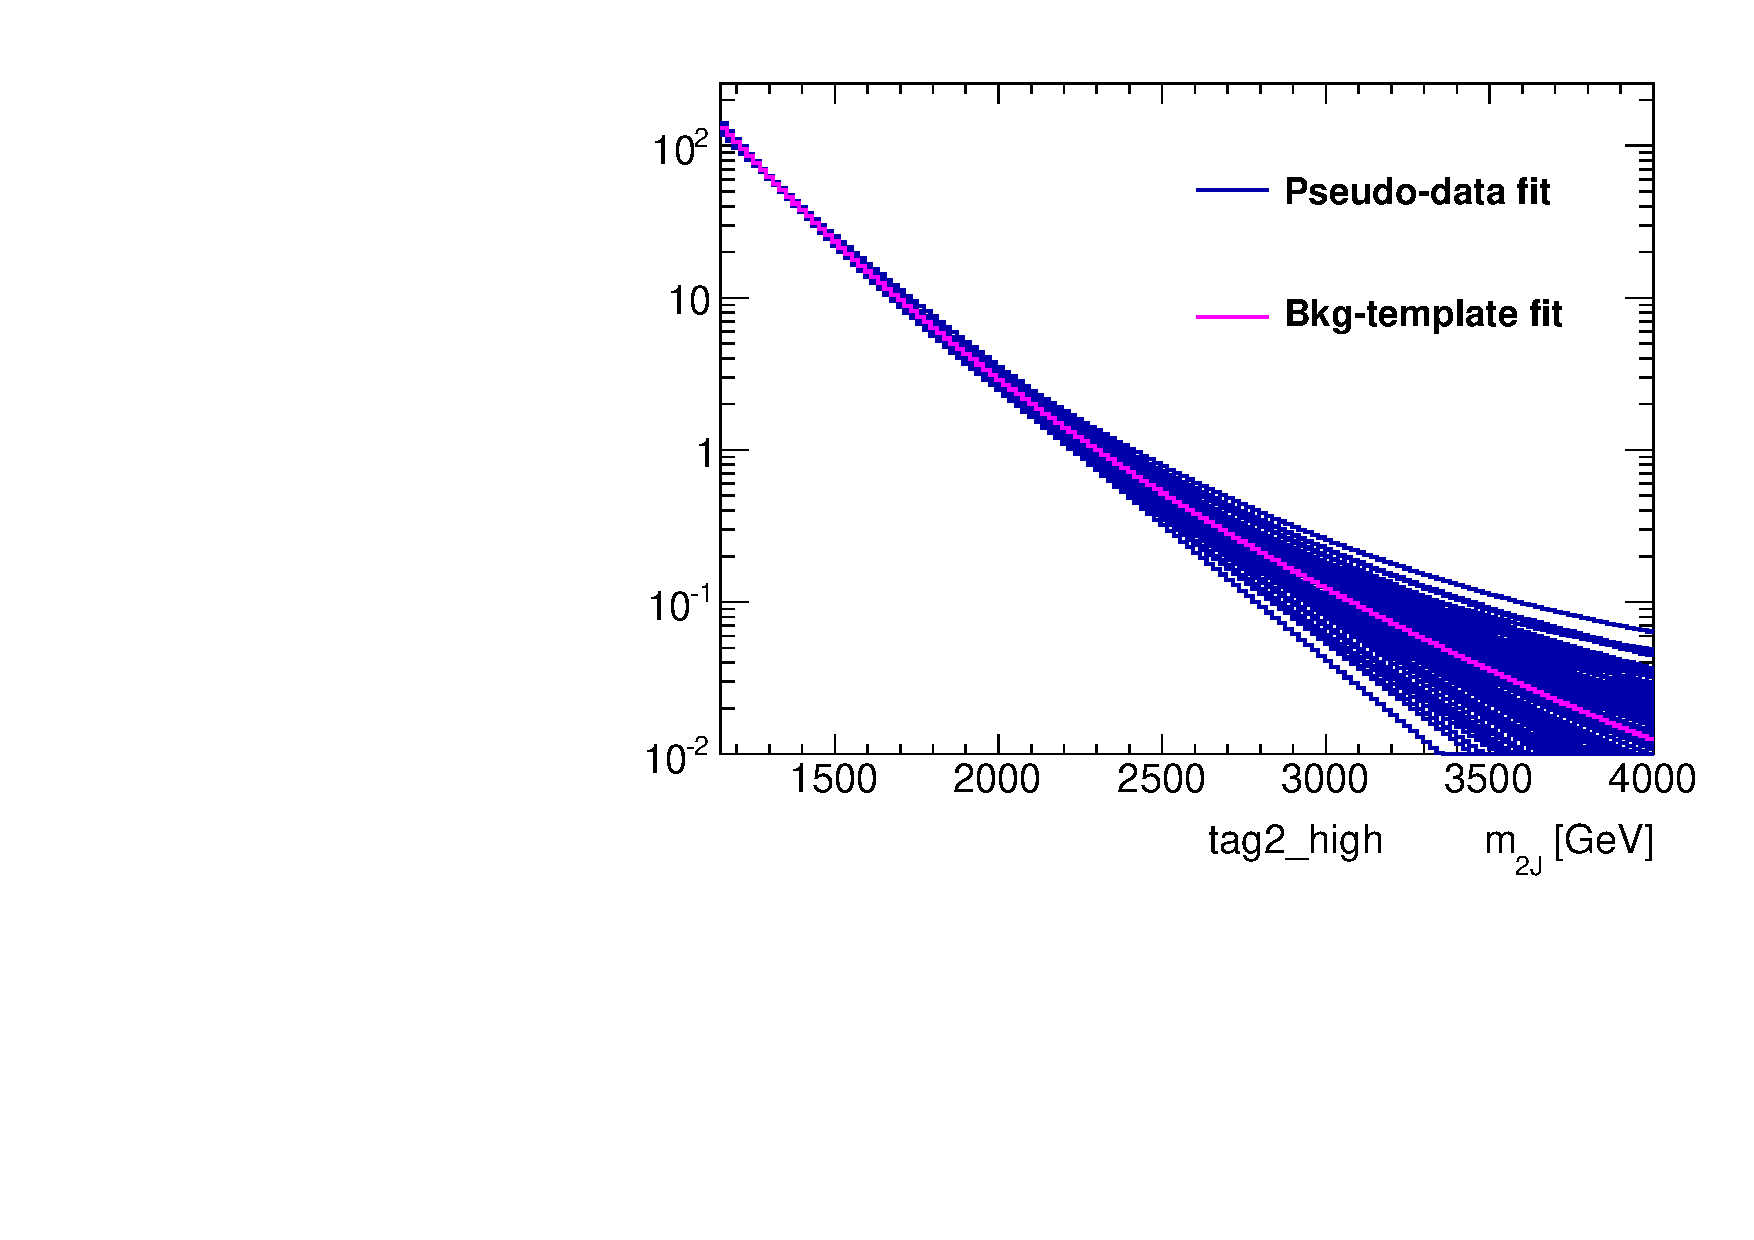
\includegraphics[angle=270, width=0.32\textwidth]{./figures/boosted/app-directfit/overlay_bonly_tag2_high.pdf} }
\subfloat[]{ 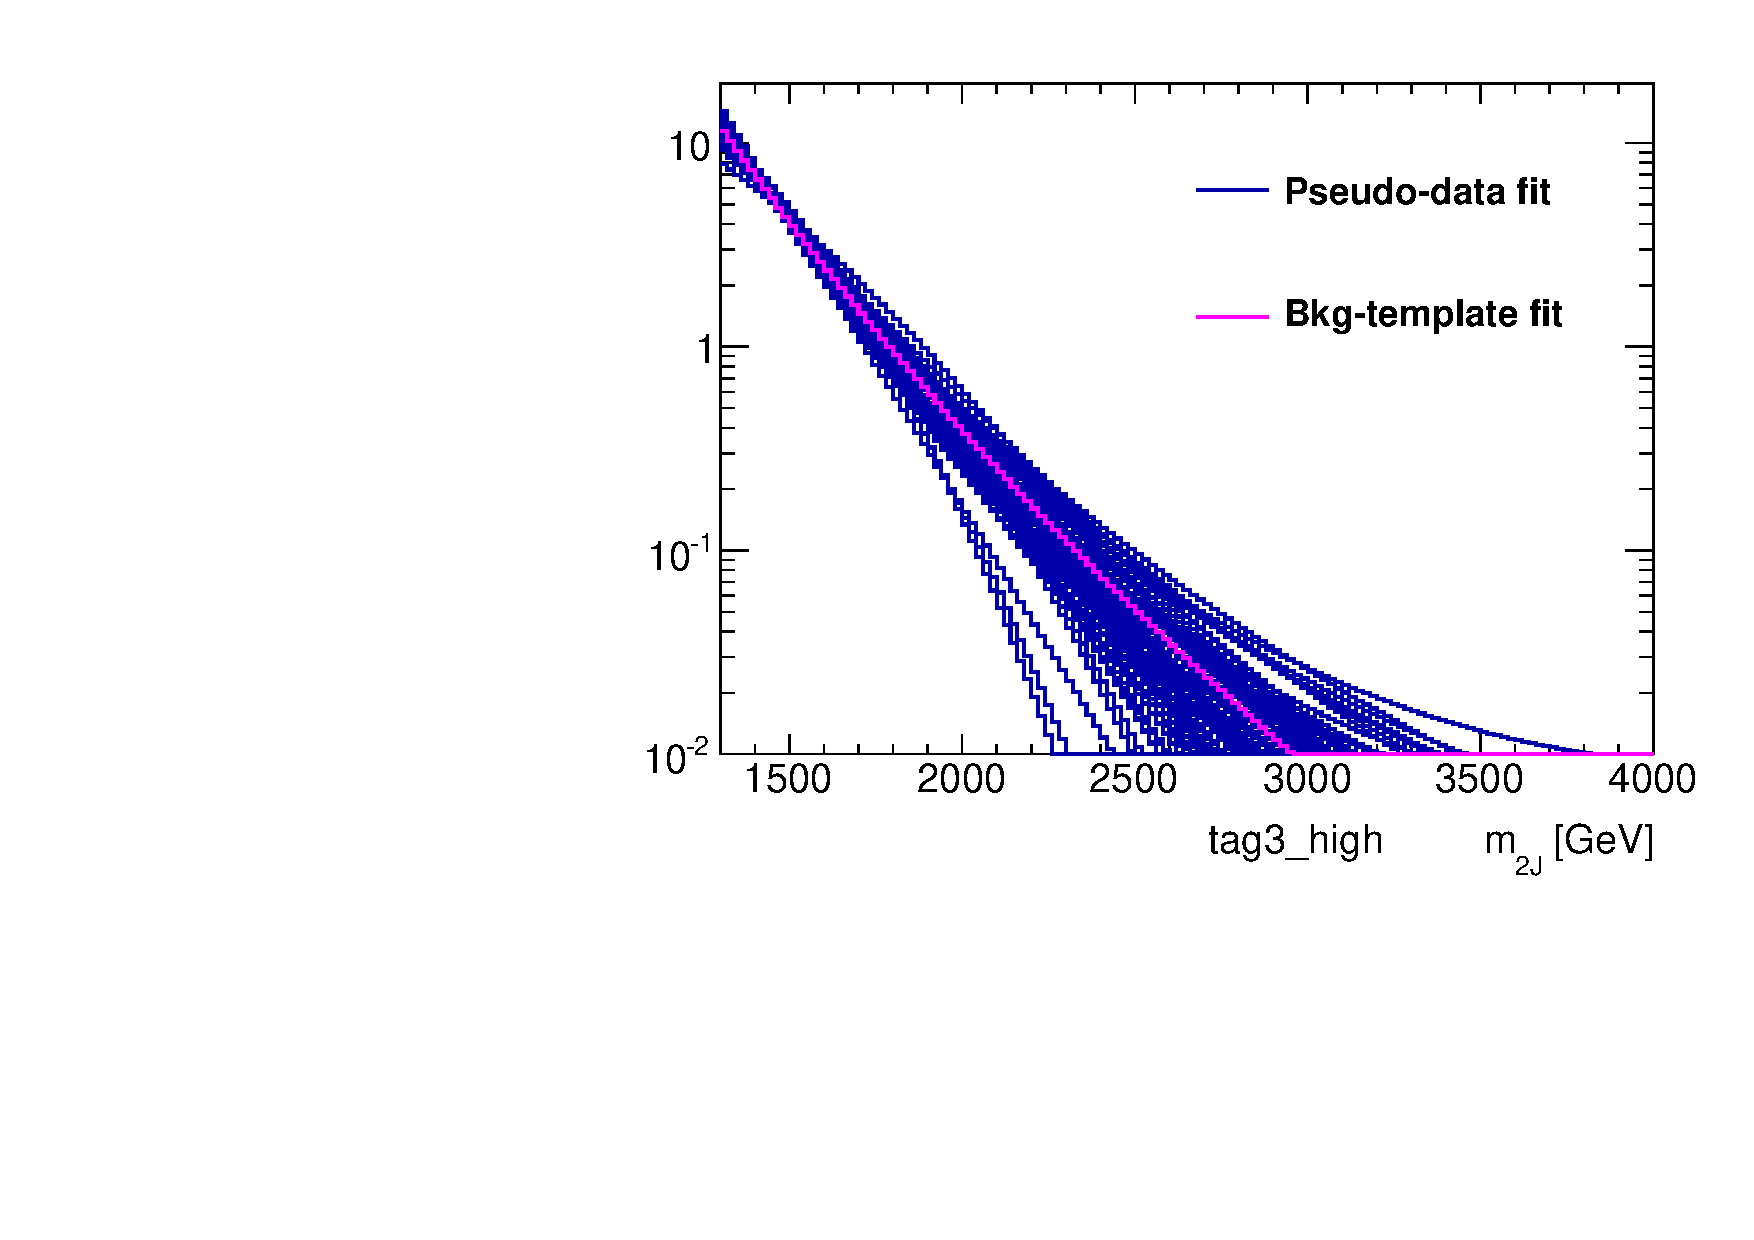
\includegraphics[angle=270, width=0.32\textwidth]{./figures/boosted/app-directfit/overlay_bonly_tag3_high.pdf} }
\caption{Visualization of the background-only fits for 100 toys (in blue), and overlayed the fit to the high-stat background-templates (in pink). The categories are: (a) 2bs low mass, (b) 3b low mass, (c) 4b, (d) 2bs high mass and (e) 3b high mass.}
\label{fig:directfit:pseudobkgfits}
\end{center}
\end{figure*}

The next step is to extract the eigenvariations from the covariance matrix from the background-only fits. The relative difference of these variations wrt. the nominal background is displayed for each category in Fig.~\ref{fig:directfit:eigenvar2blow}-\ref{fig:directfit:eigenvar4b}. The eigenvariations from the high-stat background-templates are overlayed with thicker solid lines. From these plots it is clear, that the variations in the 4b category can get extremely large, extending much beyond 100\% of the actual background yield. The conclusion is, that currently the 4b category does not have enough data statistics to assure stable fits. Tests with 4b included were performed, resulting in many problems with negative pdfs, non-convergence, non positiv-definit Hesse matrix and/or strong over-constraints.

\begin{figure*}[htbp!]
\begin{center}
\subfloat[]{ 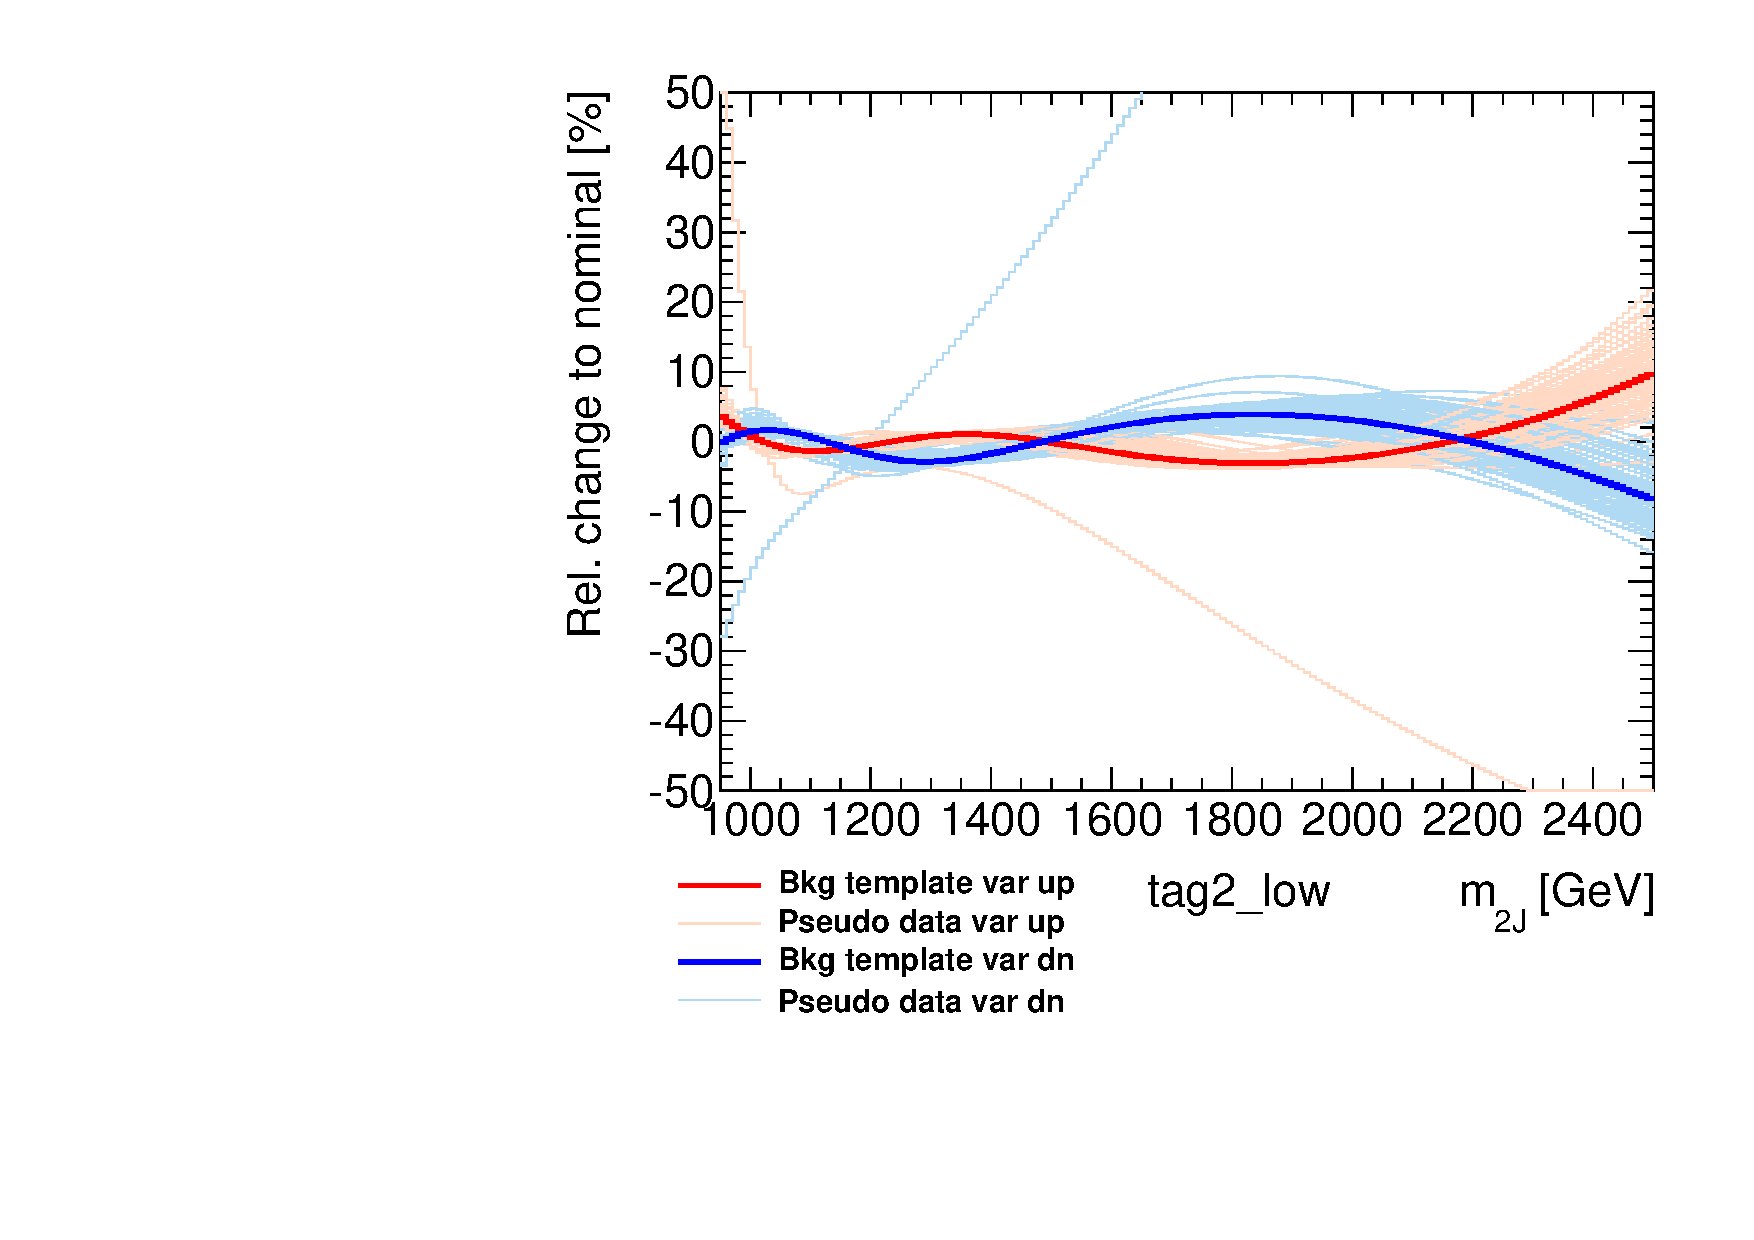
\includegraphics[angle=270, width=0.49\textwidth]{./figures/boosted/app-directfit/overlay_eigenvar1_tag2_low.pdf} }
\subfloat[]{ 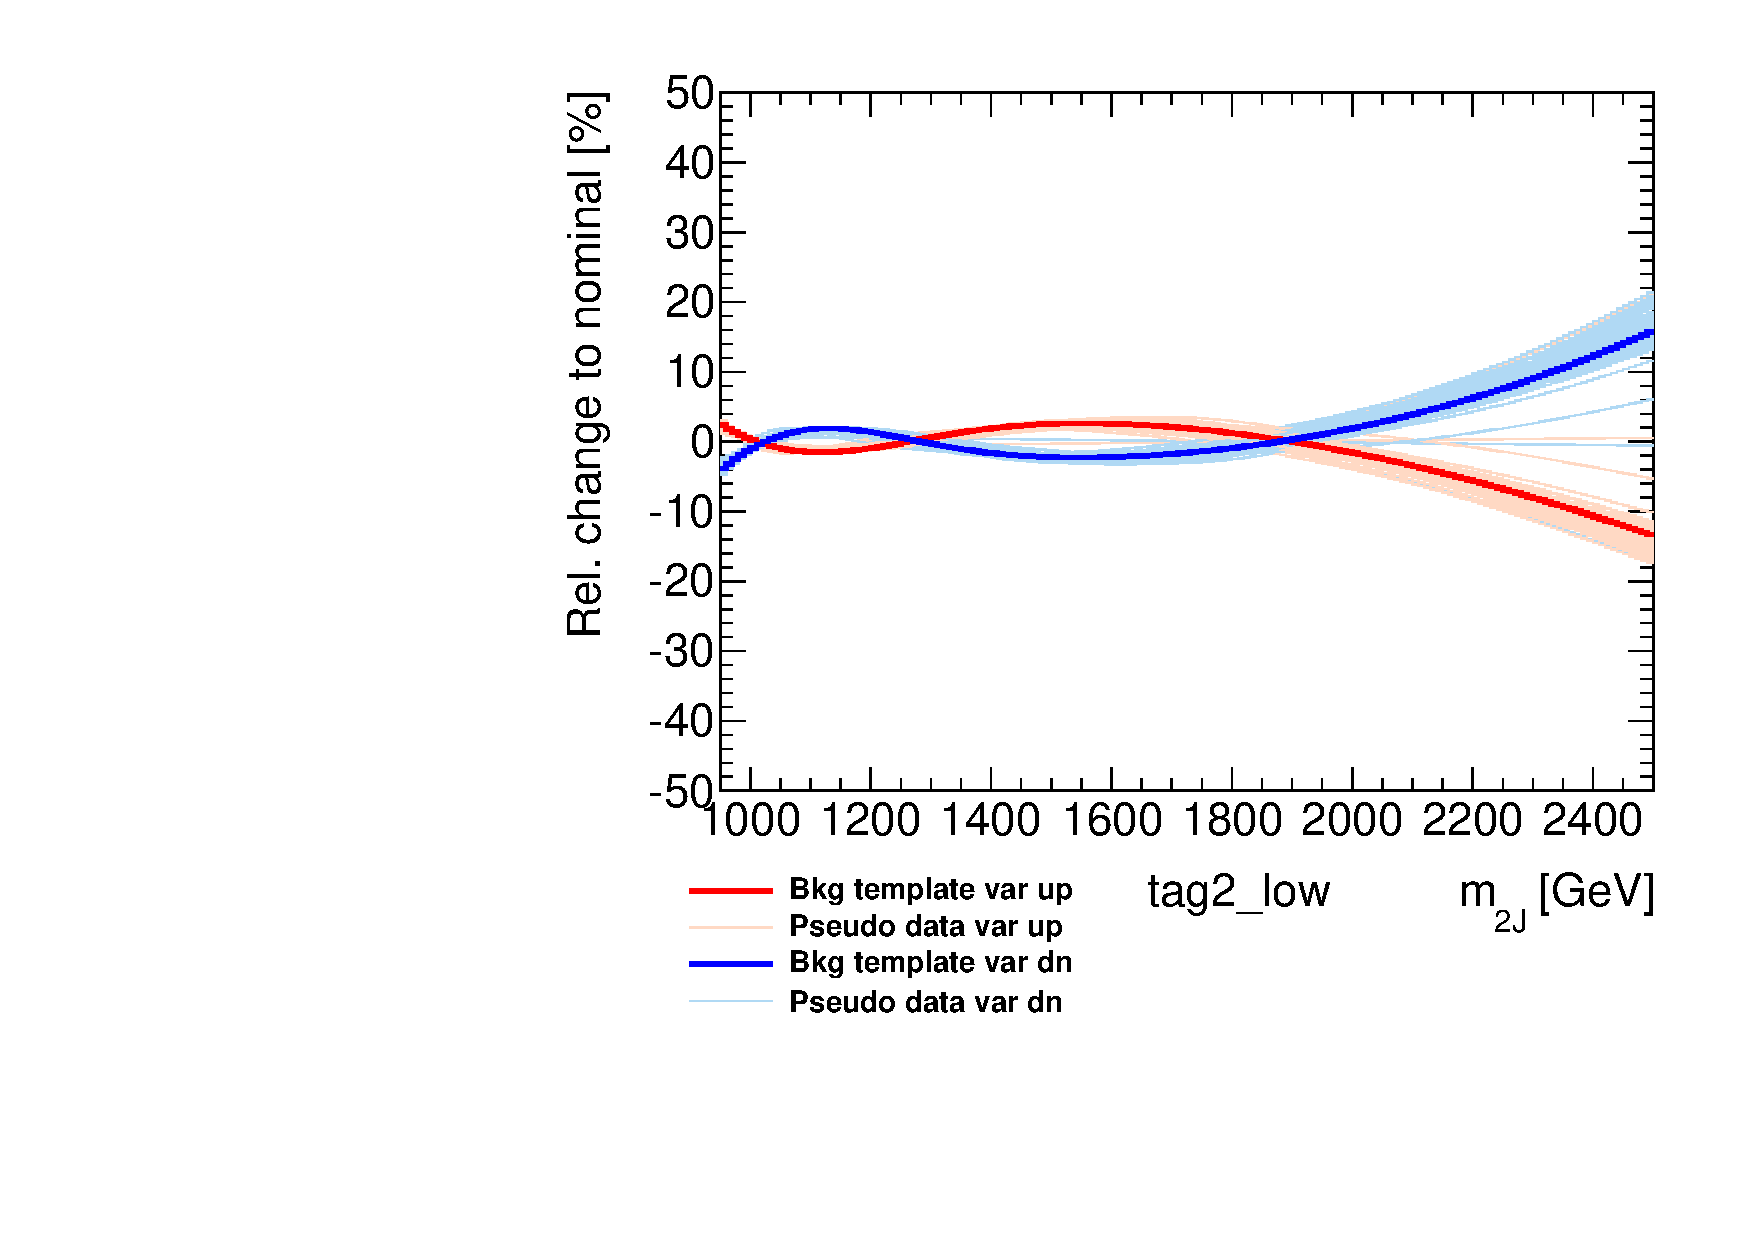
\includegraphics[angle=270, width=0.49\textwidth]{./figures/boosted/app-directfit/overlay_eigenvar2_tag2_low.pdf} } \\
\subfloat[]{ 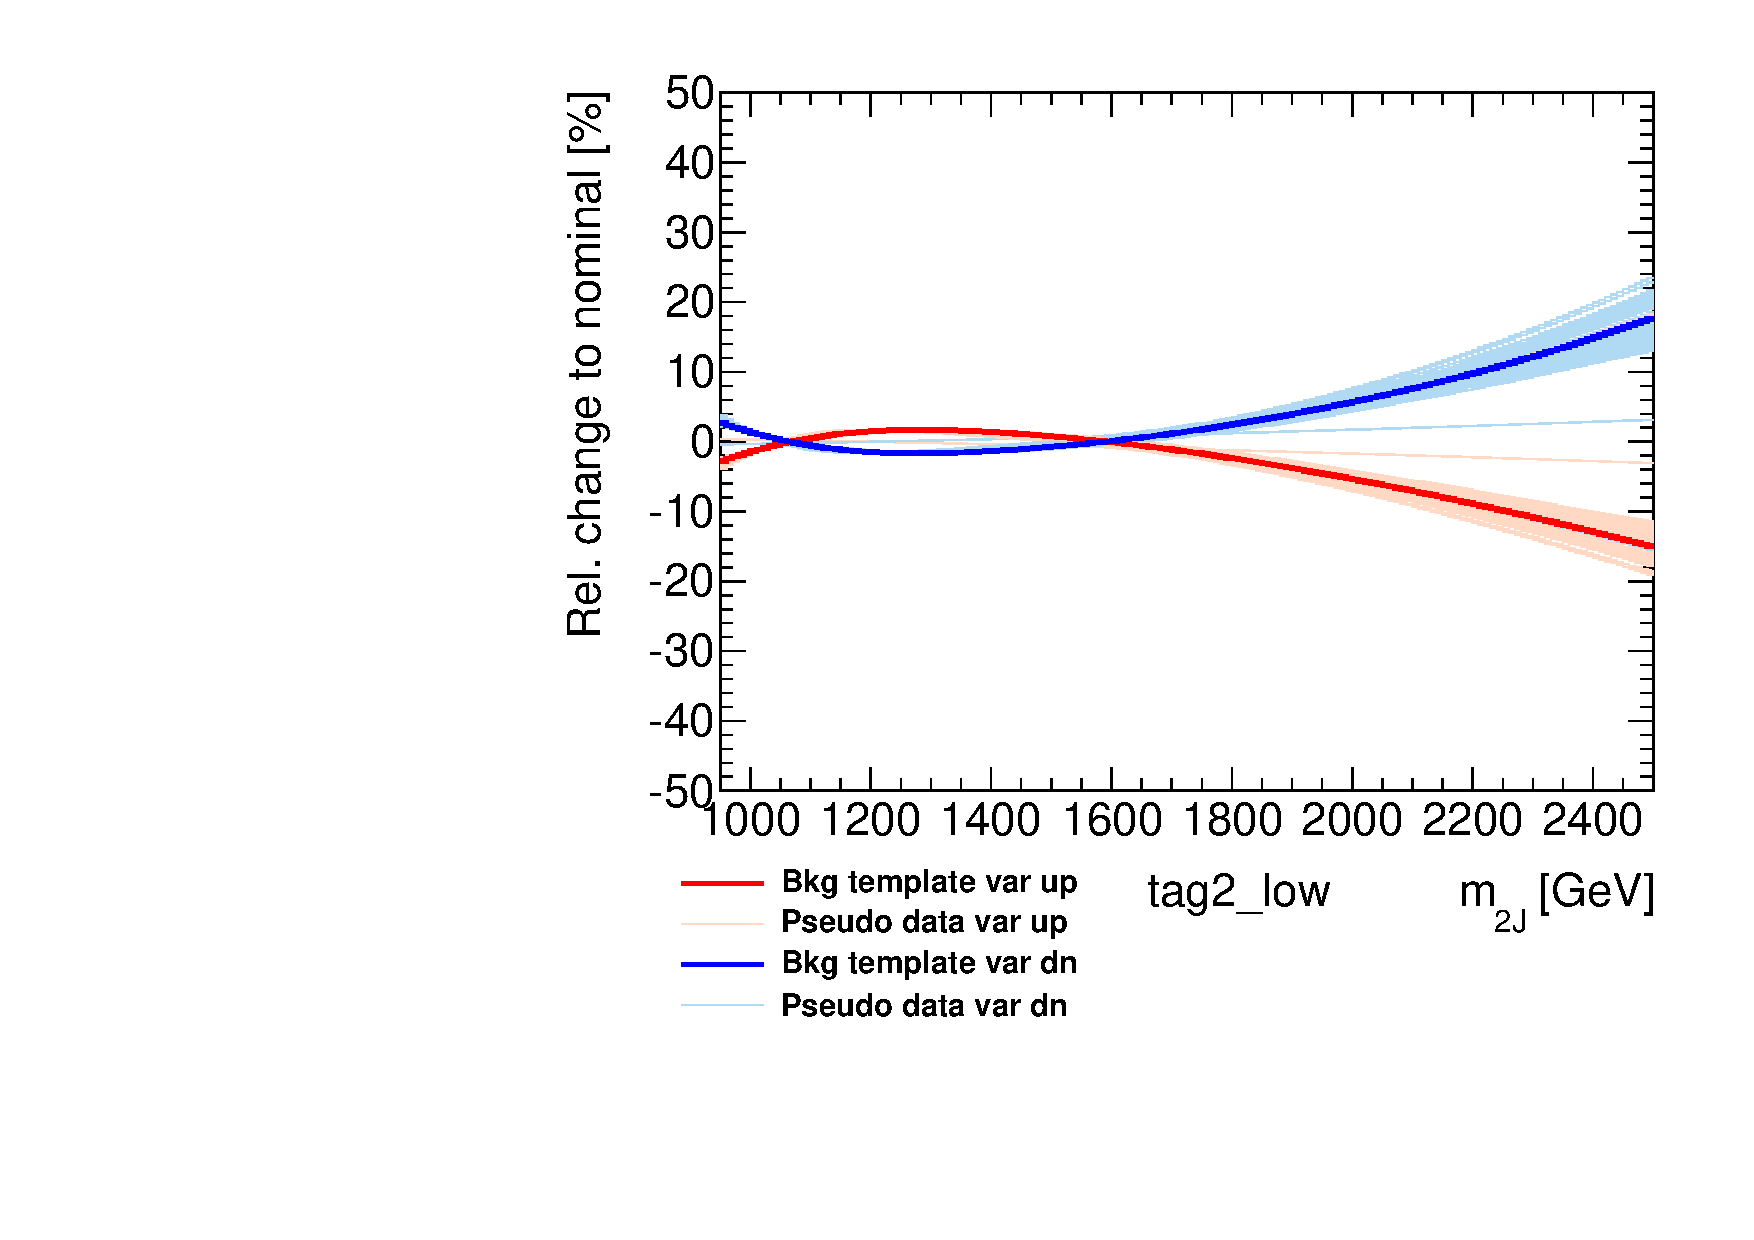
\includegraphics[angle=270, width=0.49\textwidth]{./figures/boosted/app-directfit/overlay_eigenvar3_tag2_low.pdf} }
\subfloat[]{ 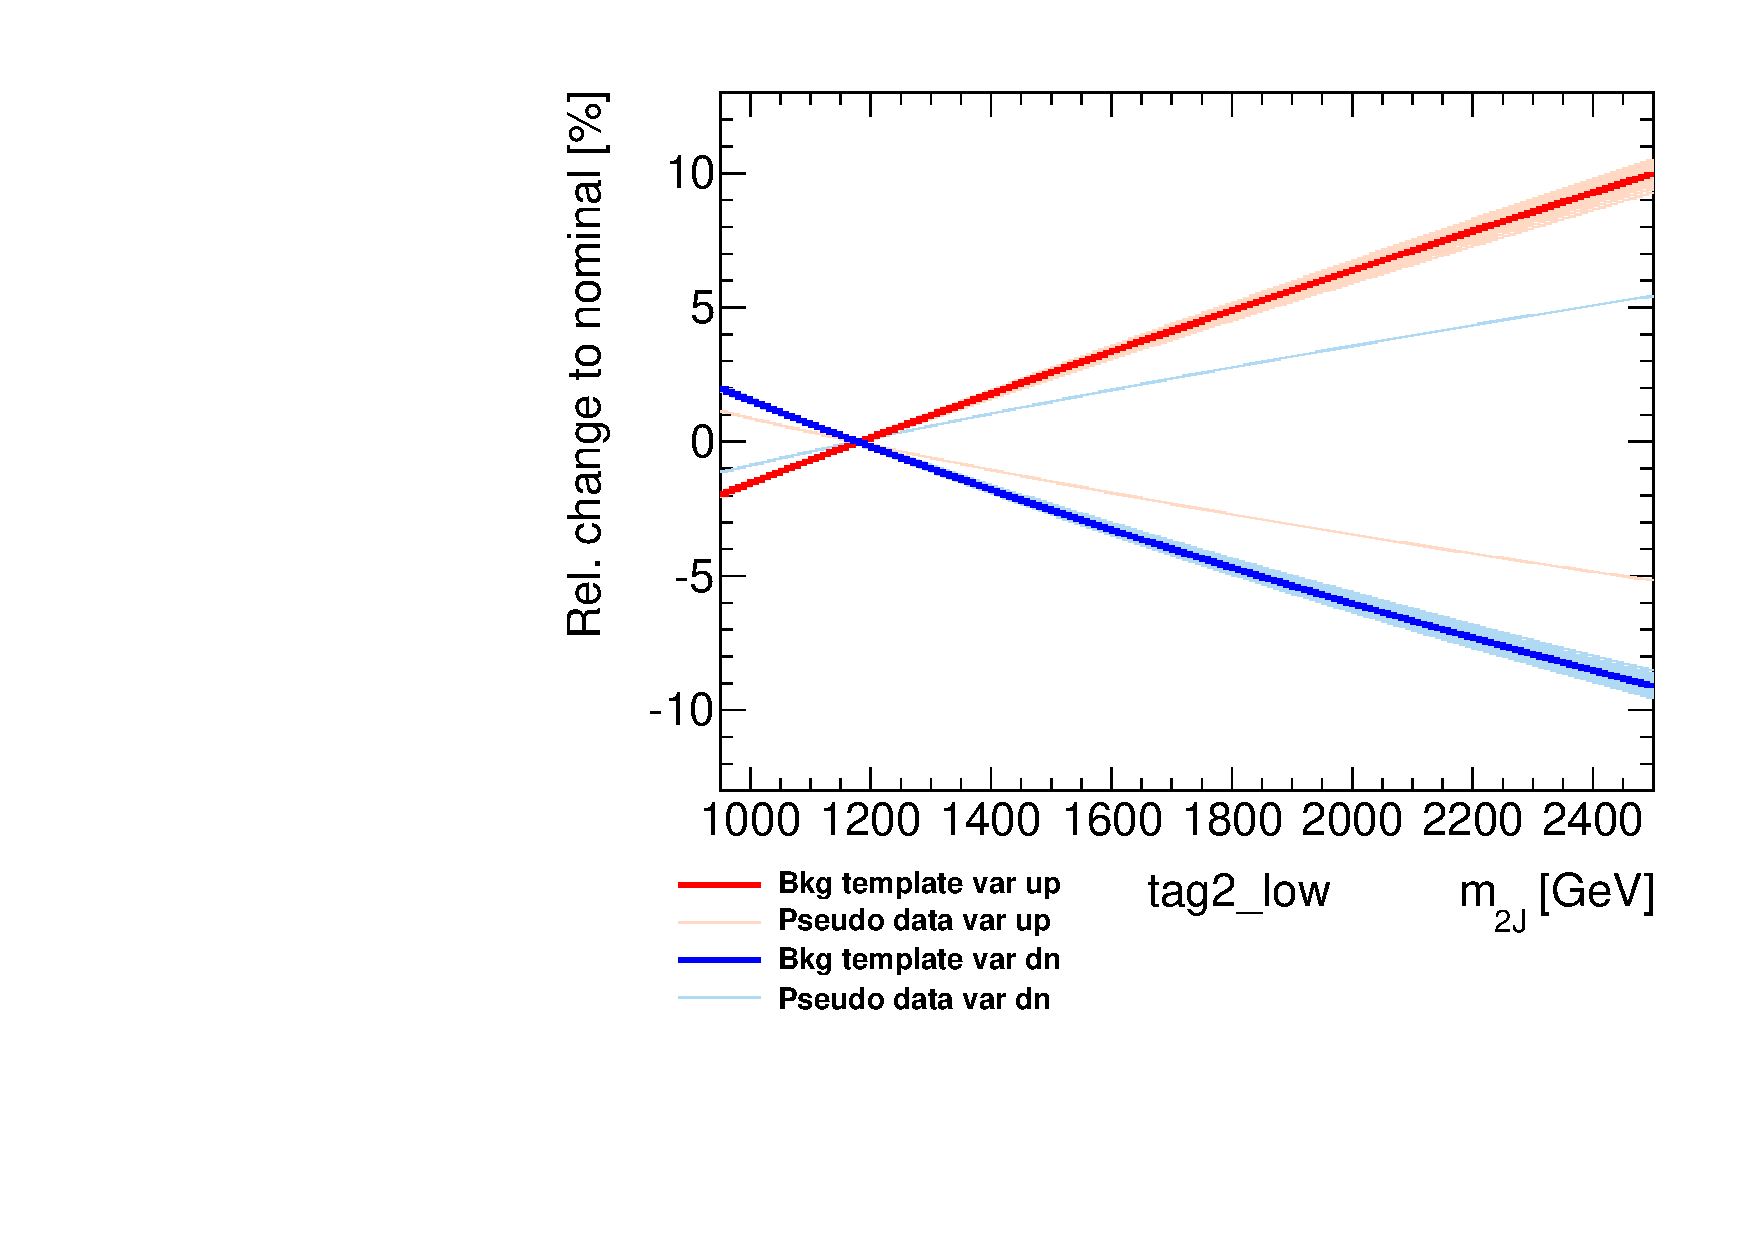
\includegraphics[angle=270, width=0.49\textwidth]{./figures/boosted/app-directfit/overlay_eigenvar4_tag2_low.pdf} }
\caption{Visualization of the eigenvariations for the 2b low mass category (function has 4 parameters). (a) shows variation 1, (b) Var2, (c) Var3 and (d) Var4.}
\label{fig:directfit:eigenvar2blow}
\end{center}
\end{figure*}

\begin{figure*}[htbp!]
\begin{center}
\subfloat[]{ 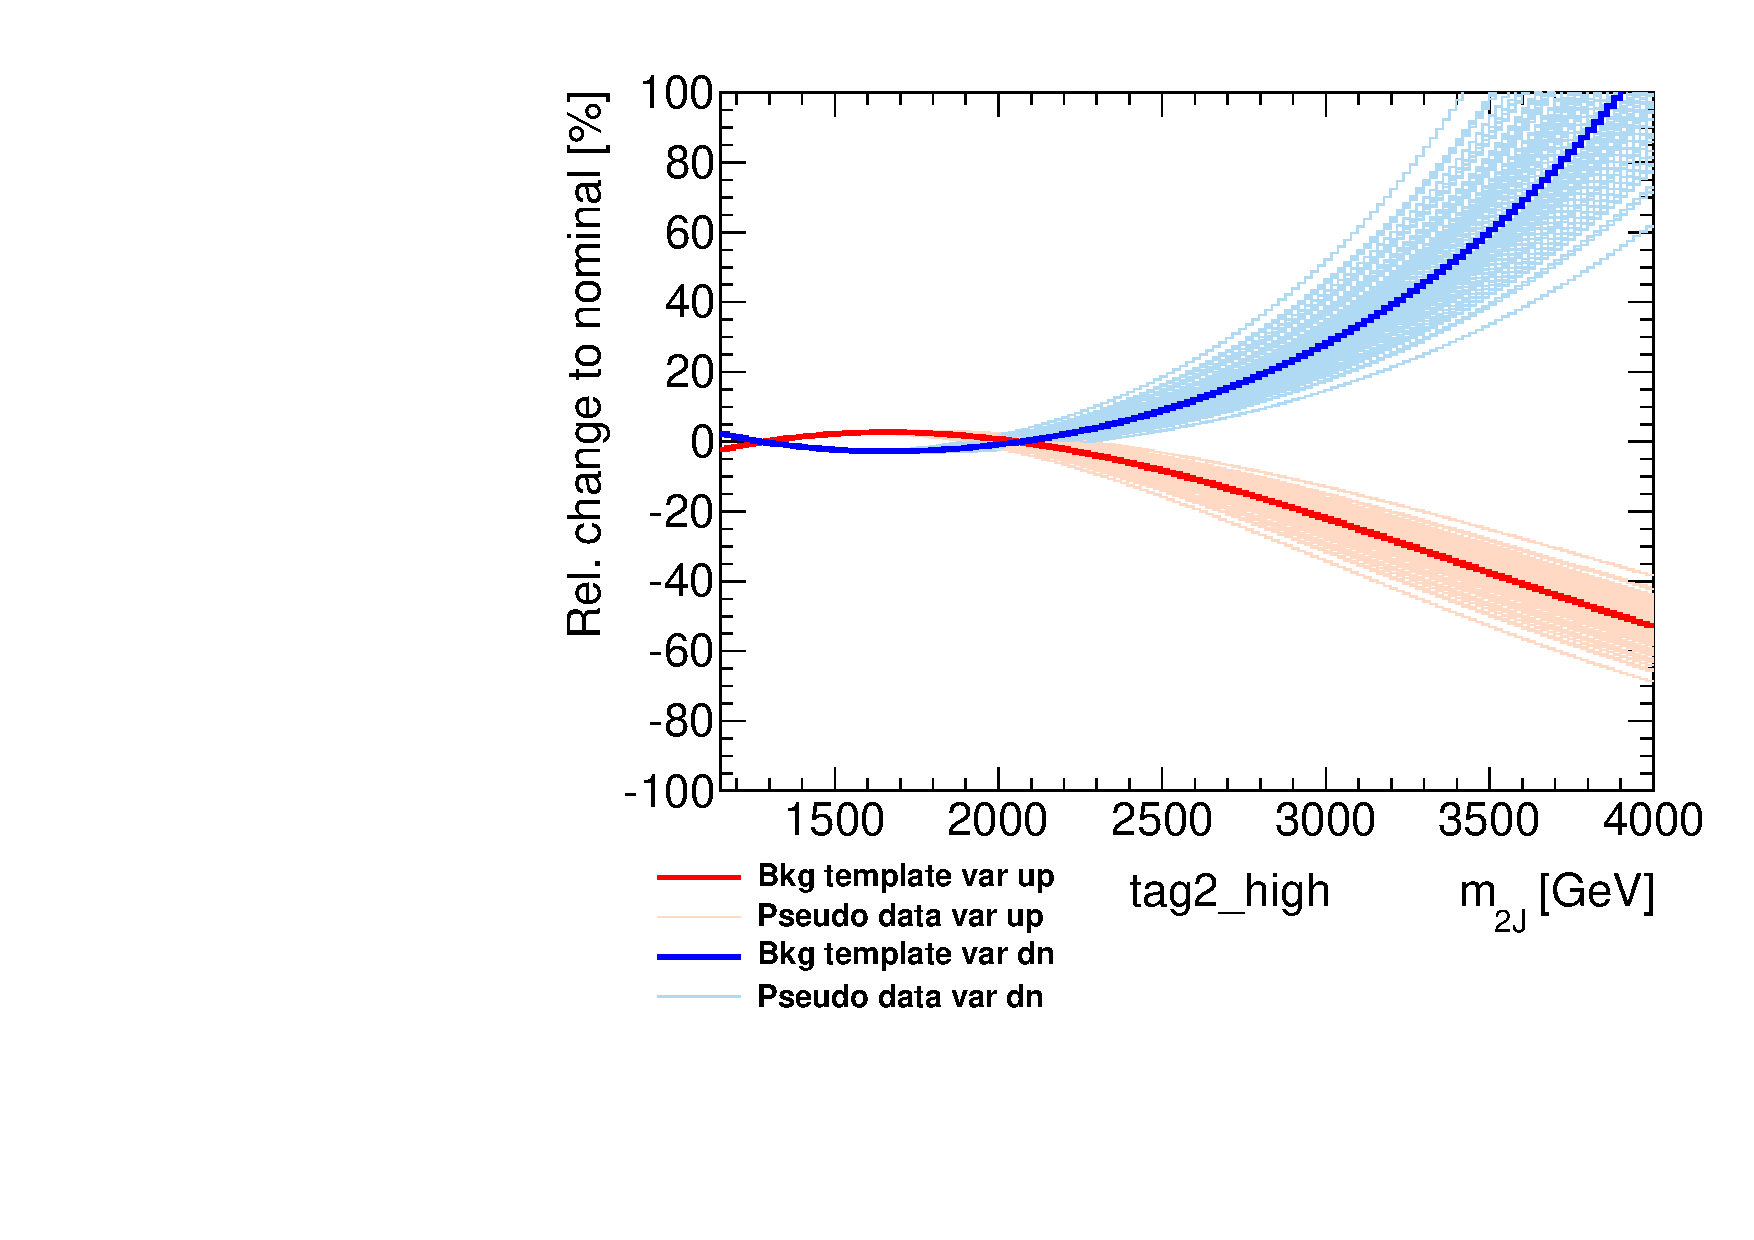
\includegraphics[angle=270, width=0.49\textwidth]{./figures/boosted/app-directfit/overlay_eigenvar1_tag2_high.pdf} }
\subfloat[]{ 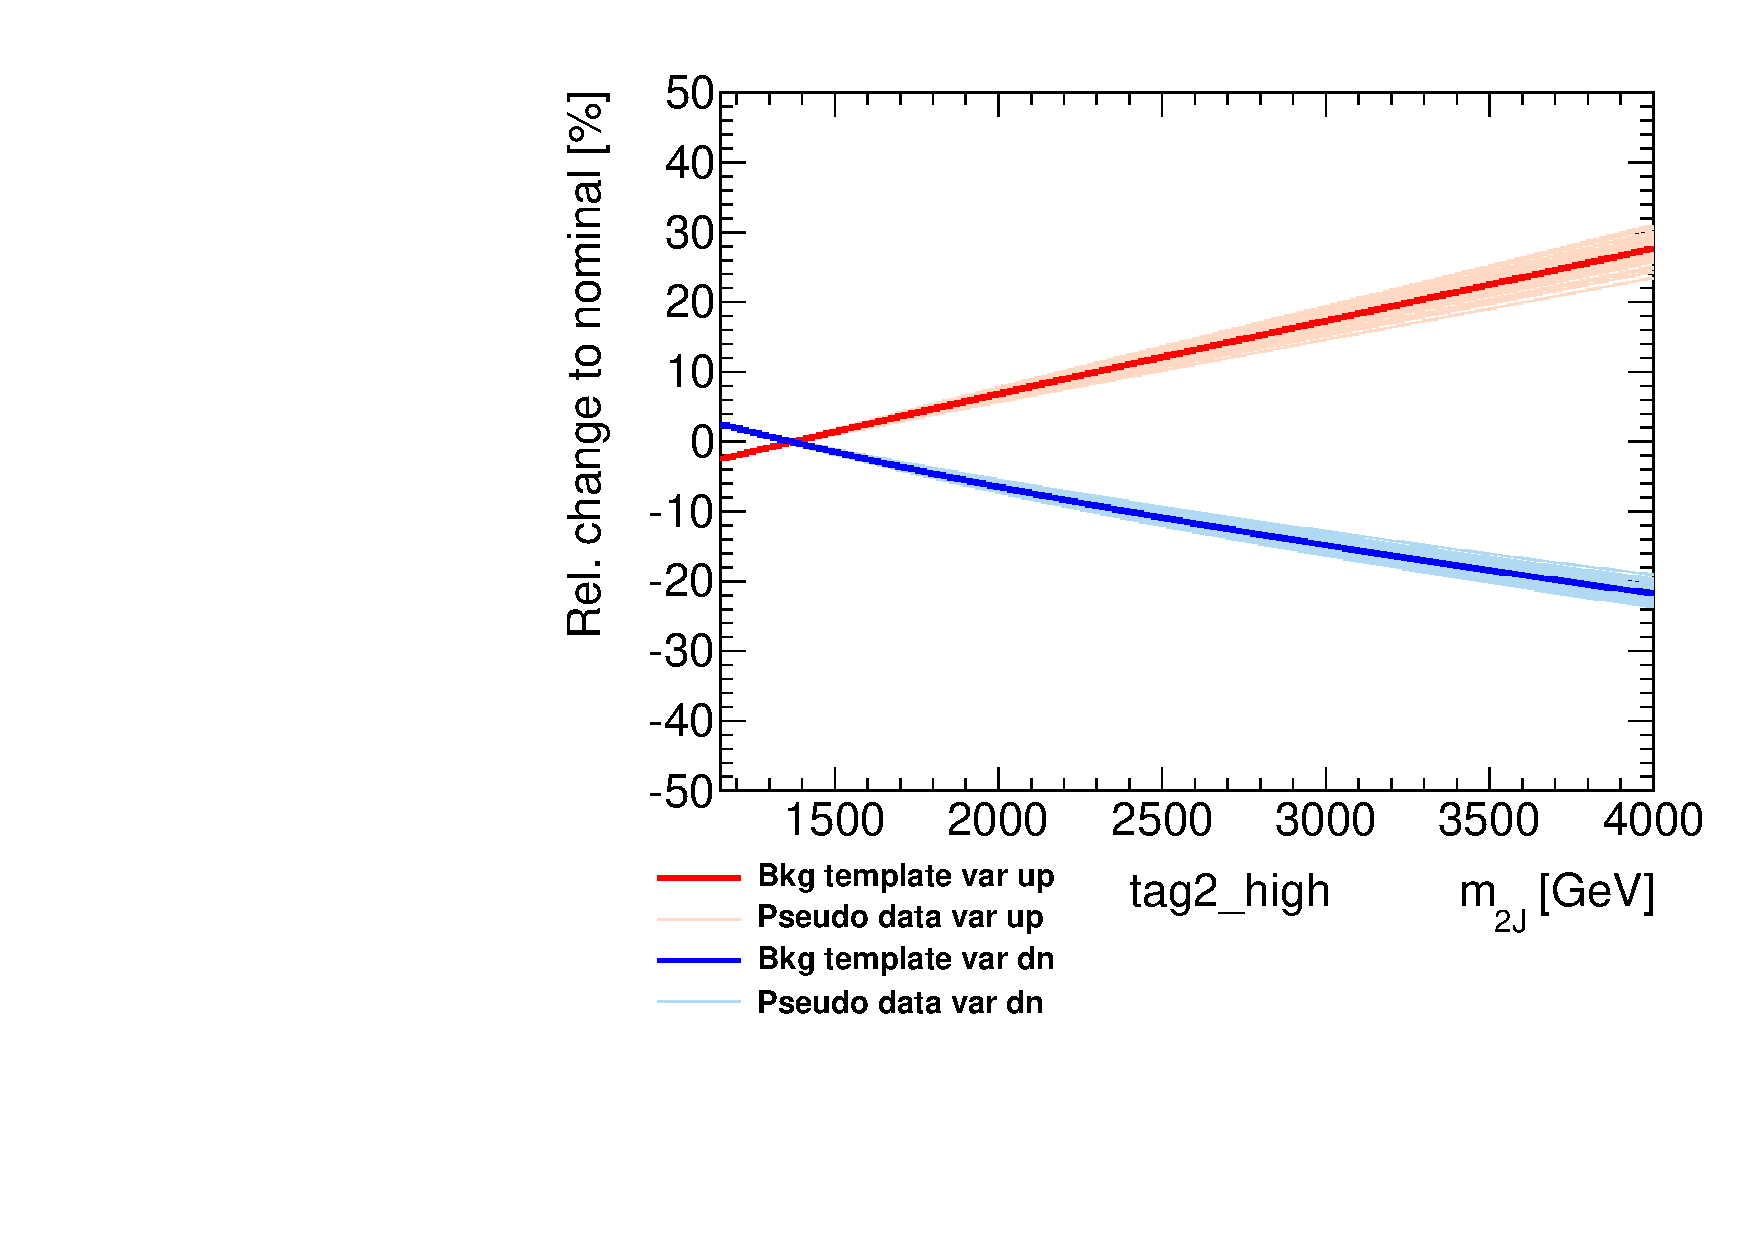
\includegraphics[angle=270, width=0.49\textwidth]{./figures/boosted/app-directfit/overlay_eigenvar2_tag2_high.pdf} }
\caption{Visualization of the eigenvariations for the 2b high mass category (function has 2 parameters). (a) shows variation 1 and (b) Var2.}
\label{fig:directfit:eigenvar2bhigh}
\end{center}
\end{figure*}

\begin{figure*}[htbp!]
\begin{center}
\subfloat[]{ 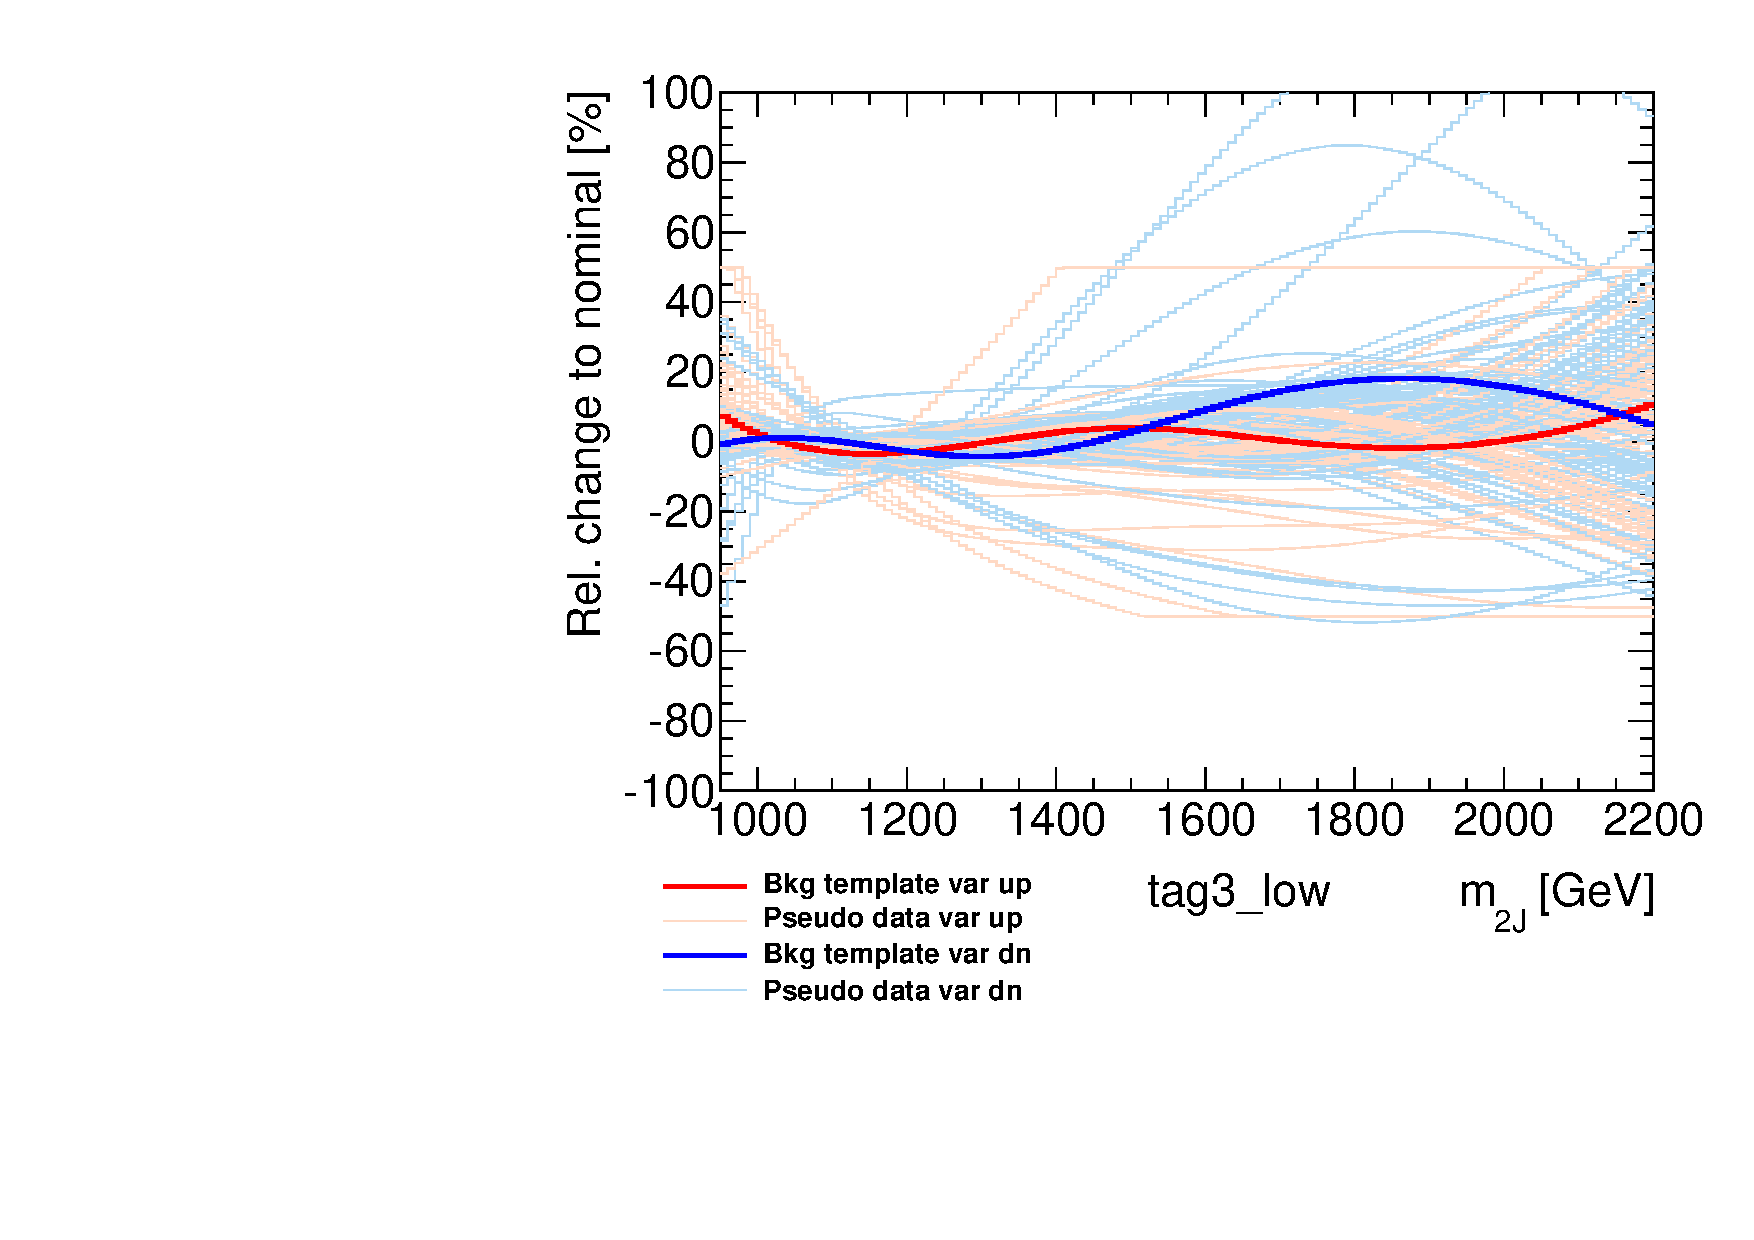
\includegraphics[angle=270, width=0.49\textwidth]{./figures/boosted/app-directfit/overlay_eigenvar1_tag3_low.pdf} }
\subfloat[]{ 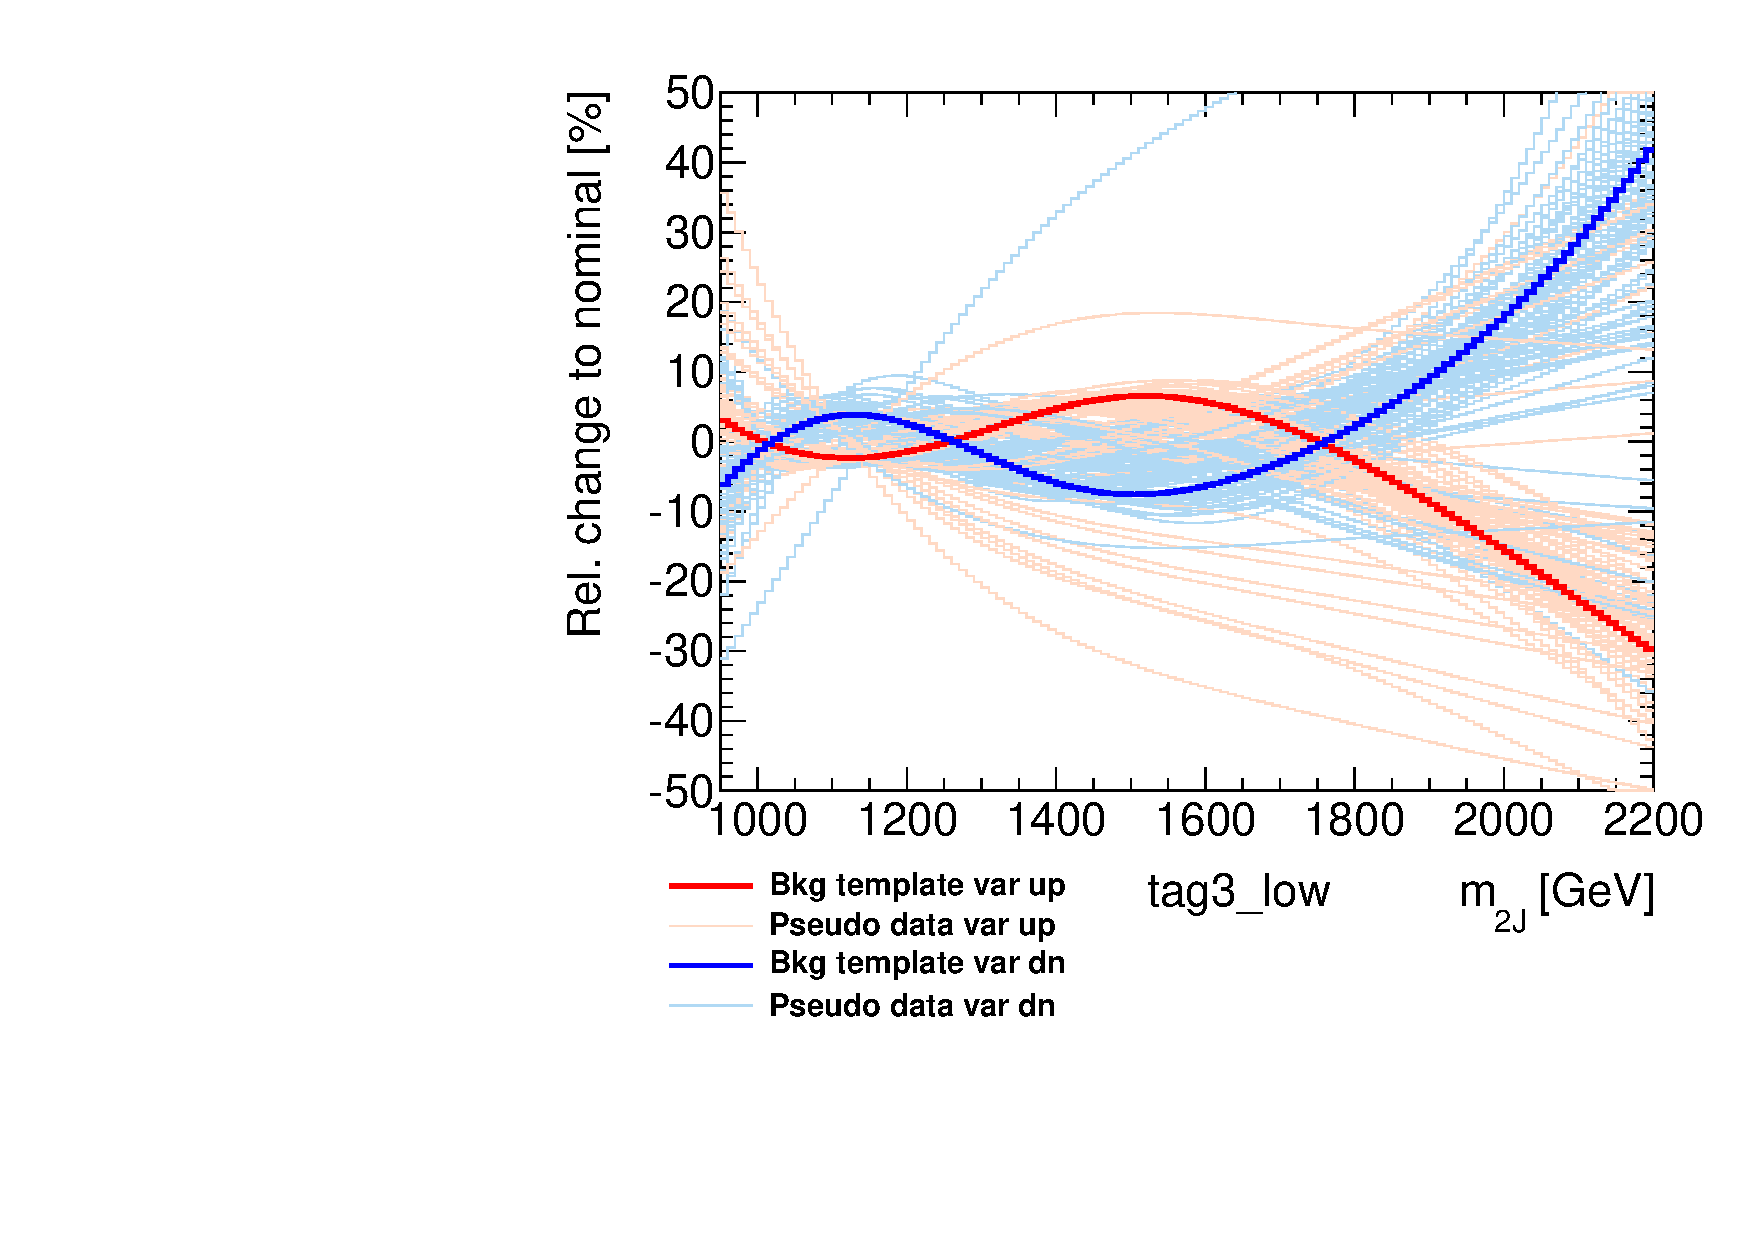
\includegraphics[angle=270, width=0.49\textwidth]{./figures/boosted/app-directfit/overlay_eigenvar2_tag3_low.pdf} } \\
\subfloat[]{ 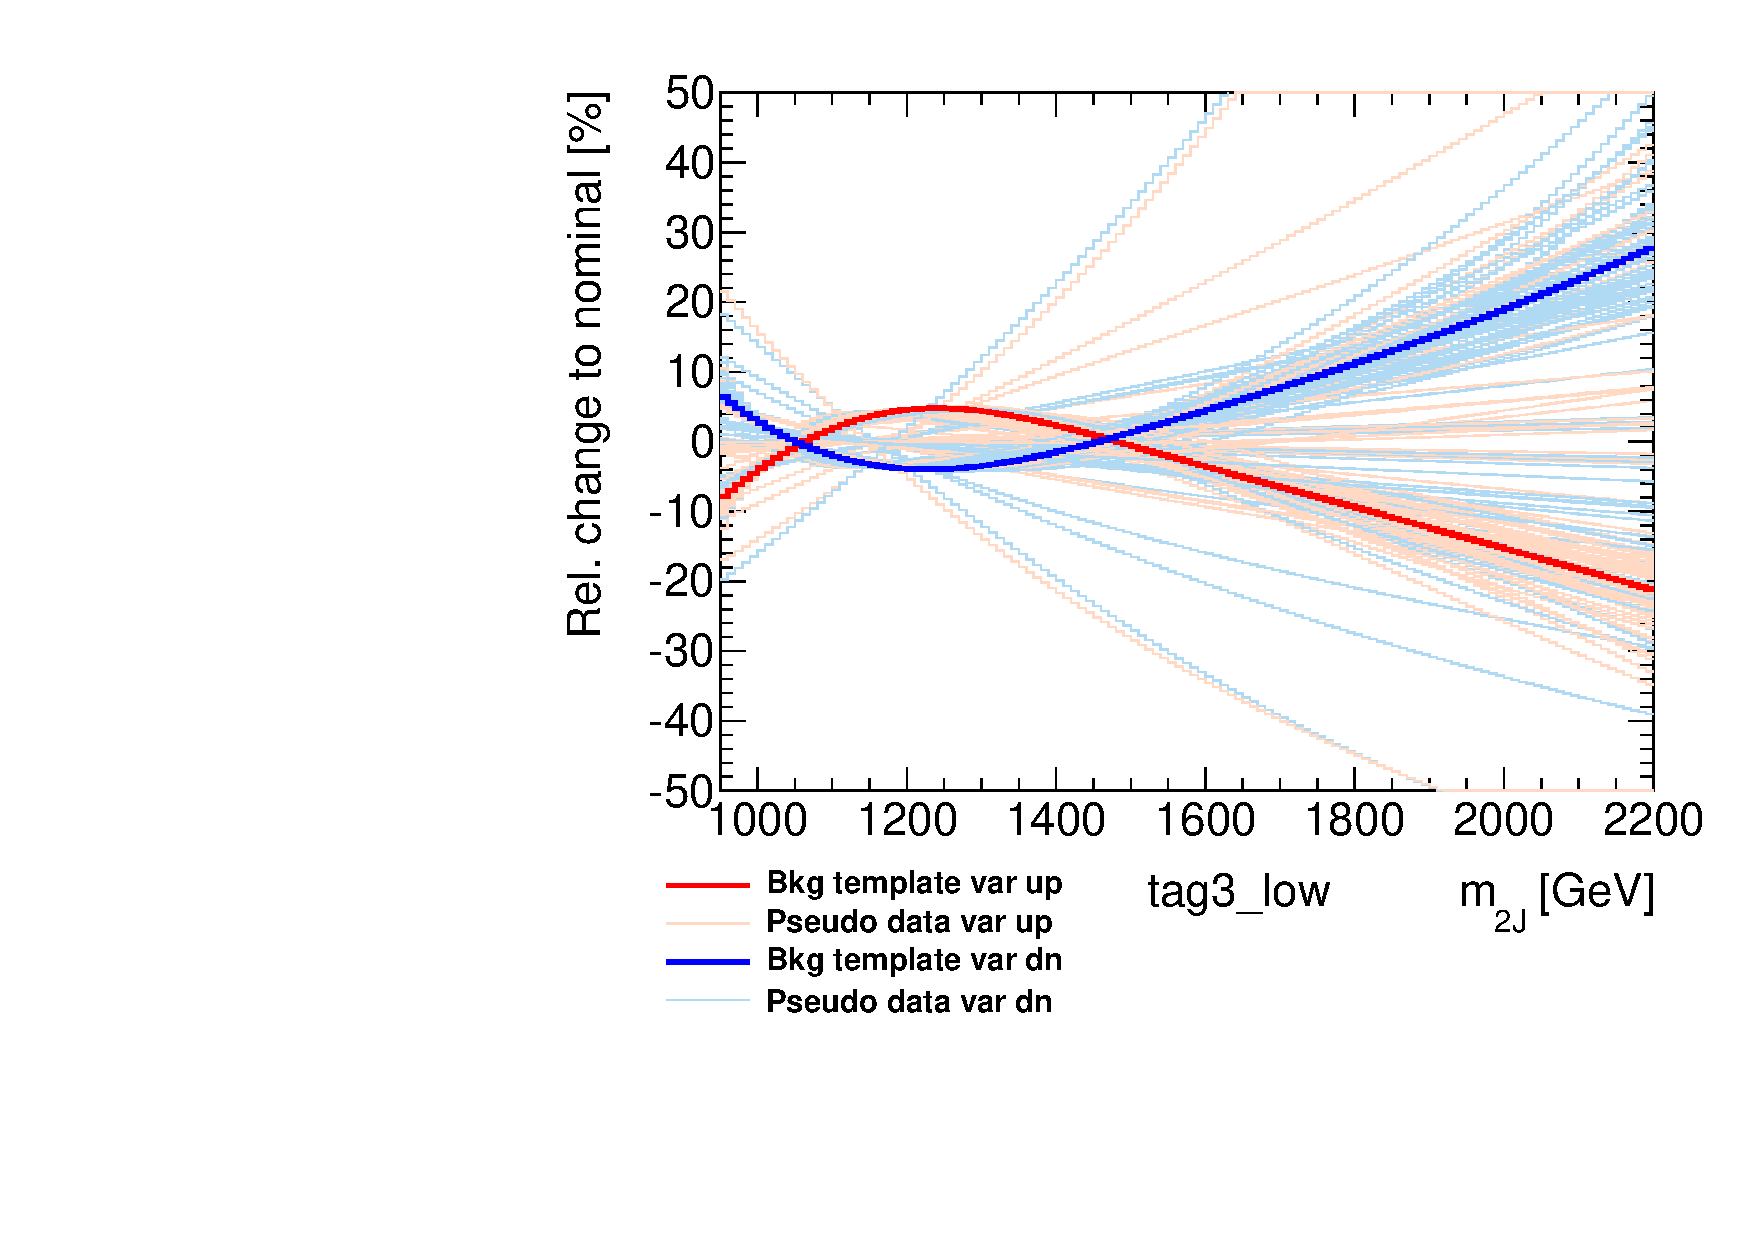
\includegraphics[angle=270, width=0.49\textwidth]{./figures/boosted/app-directfit/overlay_eigenvar3_tag3_low.pdf} }
\subfloat[]{ 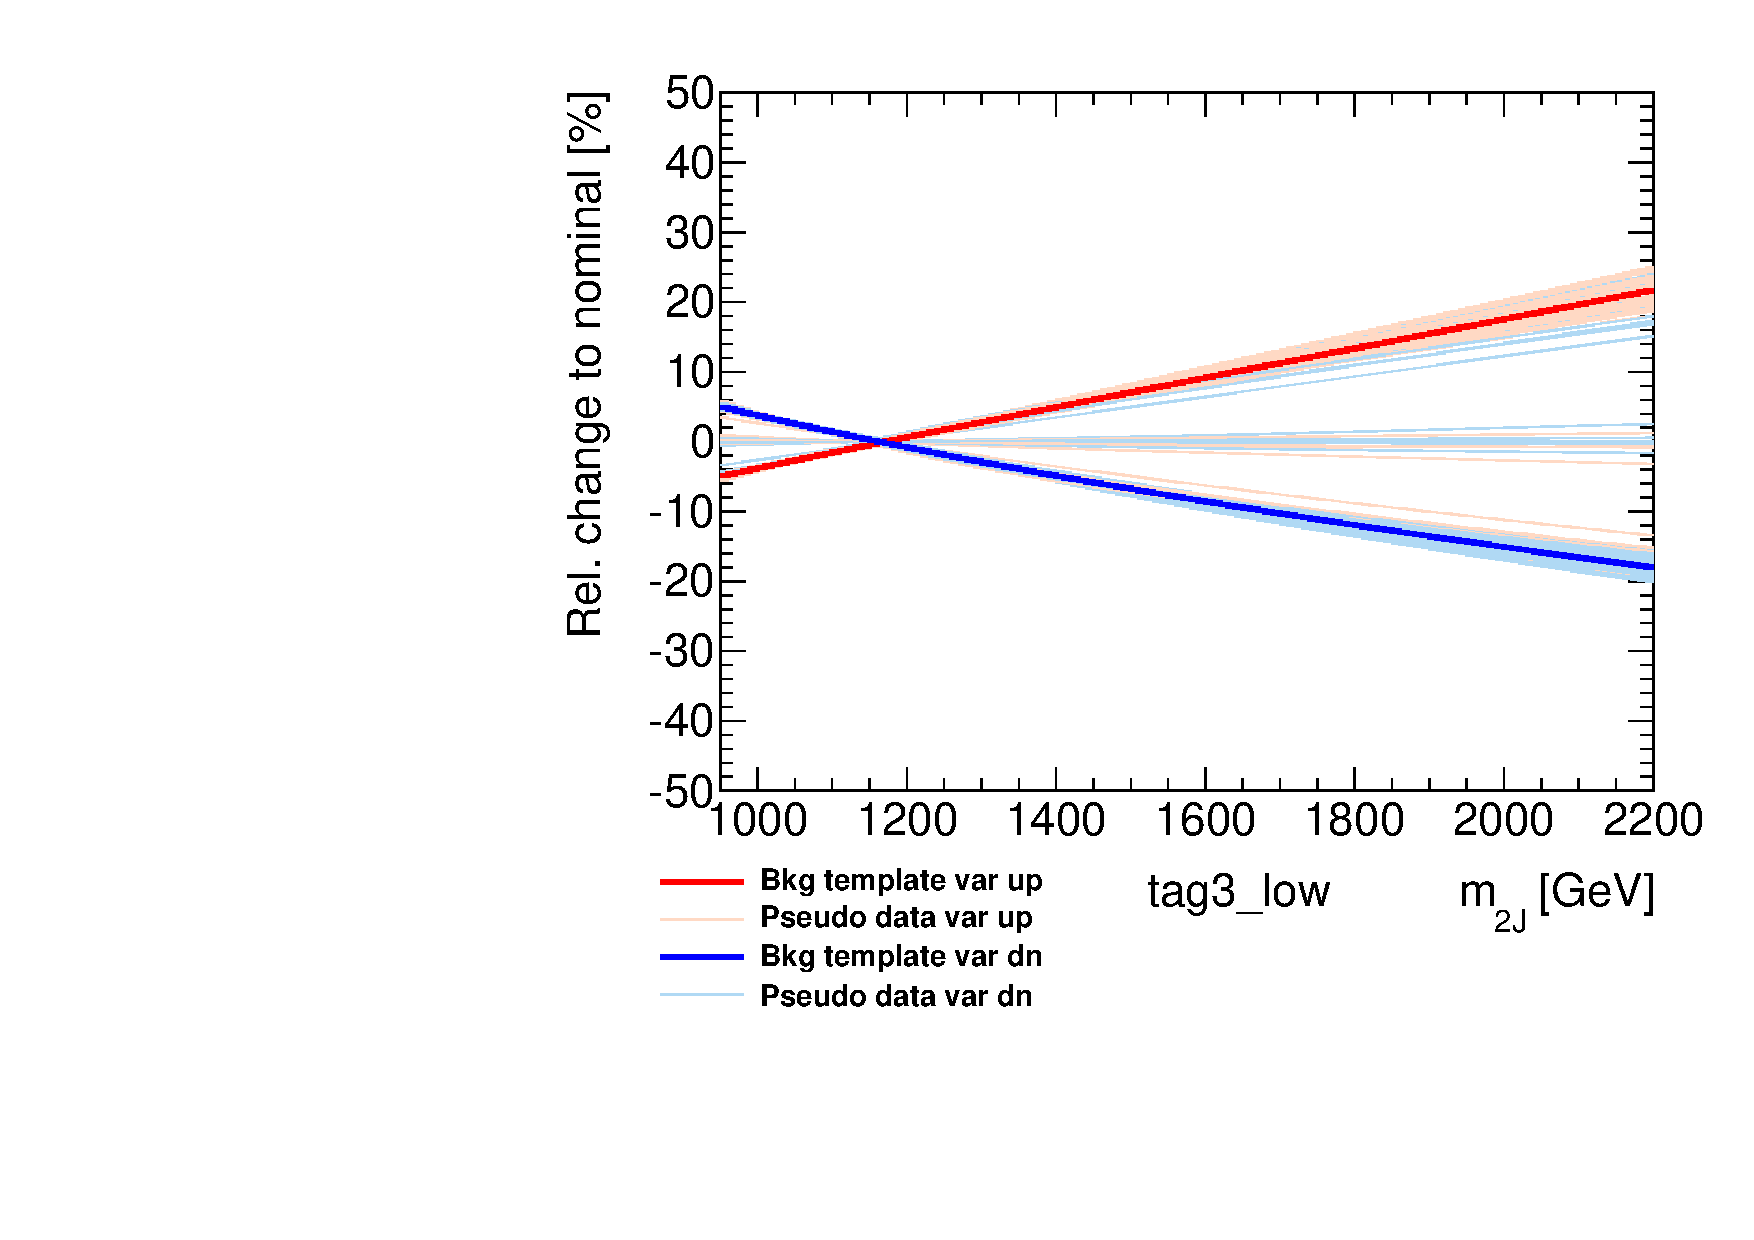
\includegraphics[angle=270, width=0.49\textwidth]{./figures/boosted/app-directfit/overlay_eigenvar4_tag3_low.pdf} }
\caption{Visualization of the eigenvariations for the 3b low mass category (function has 4 parameters). (a) shows variation 1, (b) Var2, (c) Var3 and (d) Var4.}
\label{fig:directfit:eigenvar3blow}
\end{center}
\end{figure*}

\begin{figure*}[htbp!]
\begin{center}
\subfloat[]{ 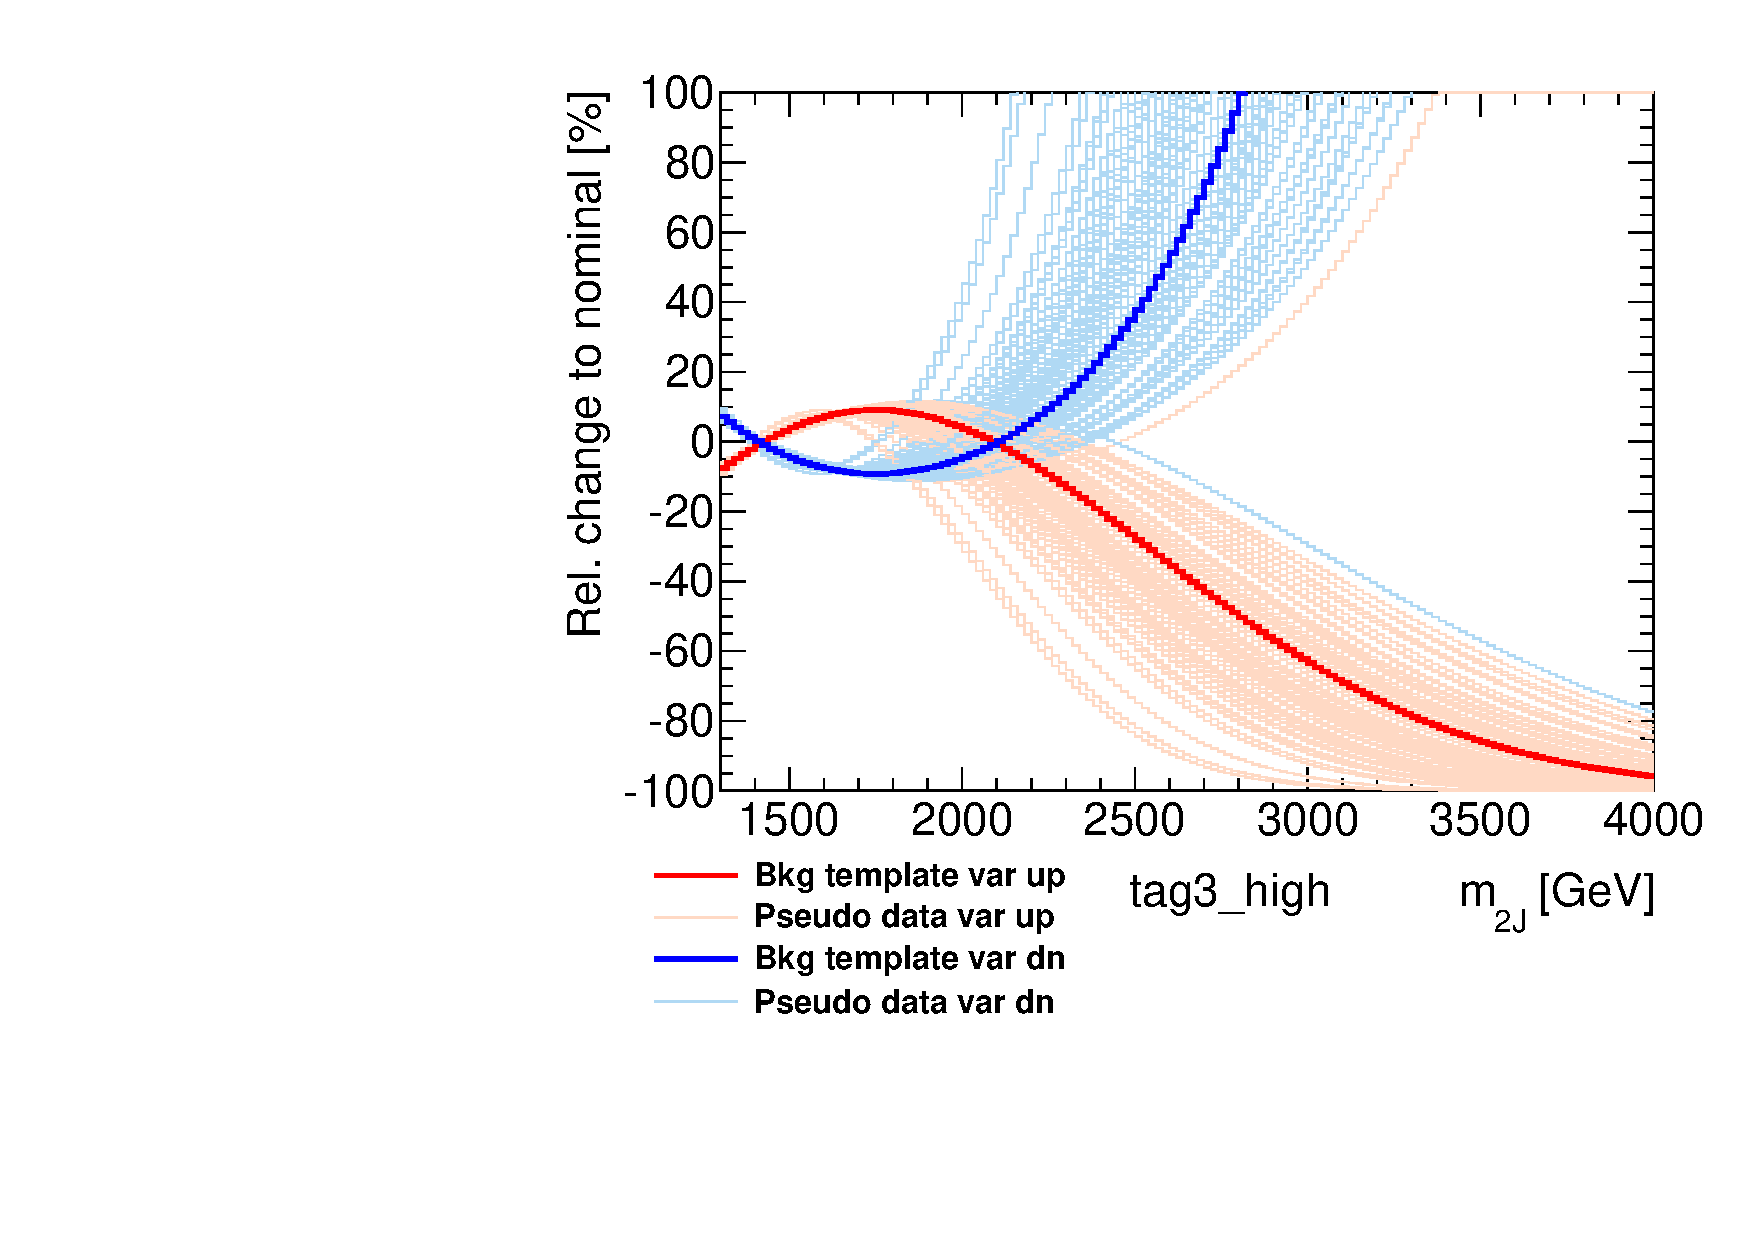
\includegraphics[angle=270, width=0.49\textwidth]{./figures/boosted/app-directfit/overlay_eigenvar1_tag3_high.pdf} }
\subfloat[]{ 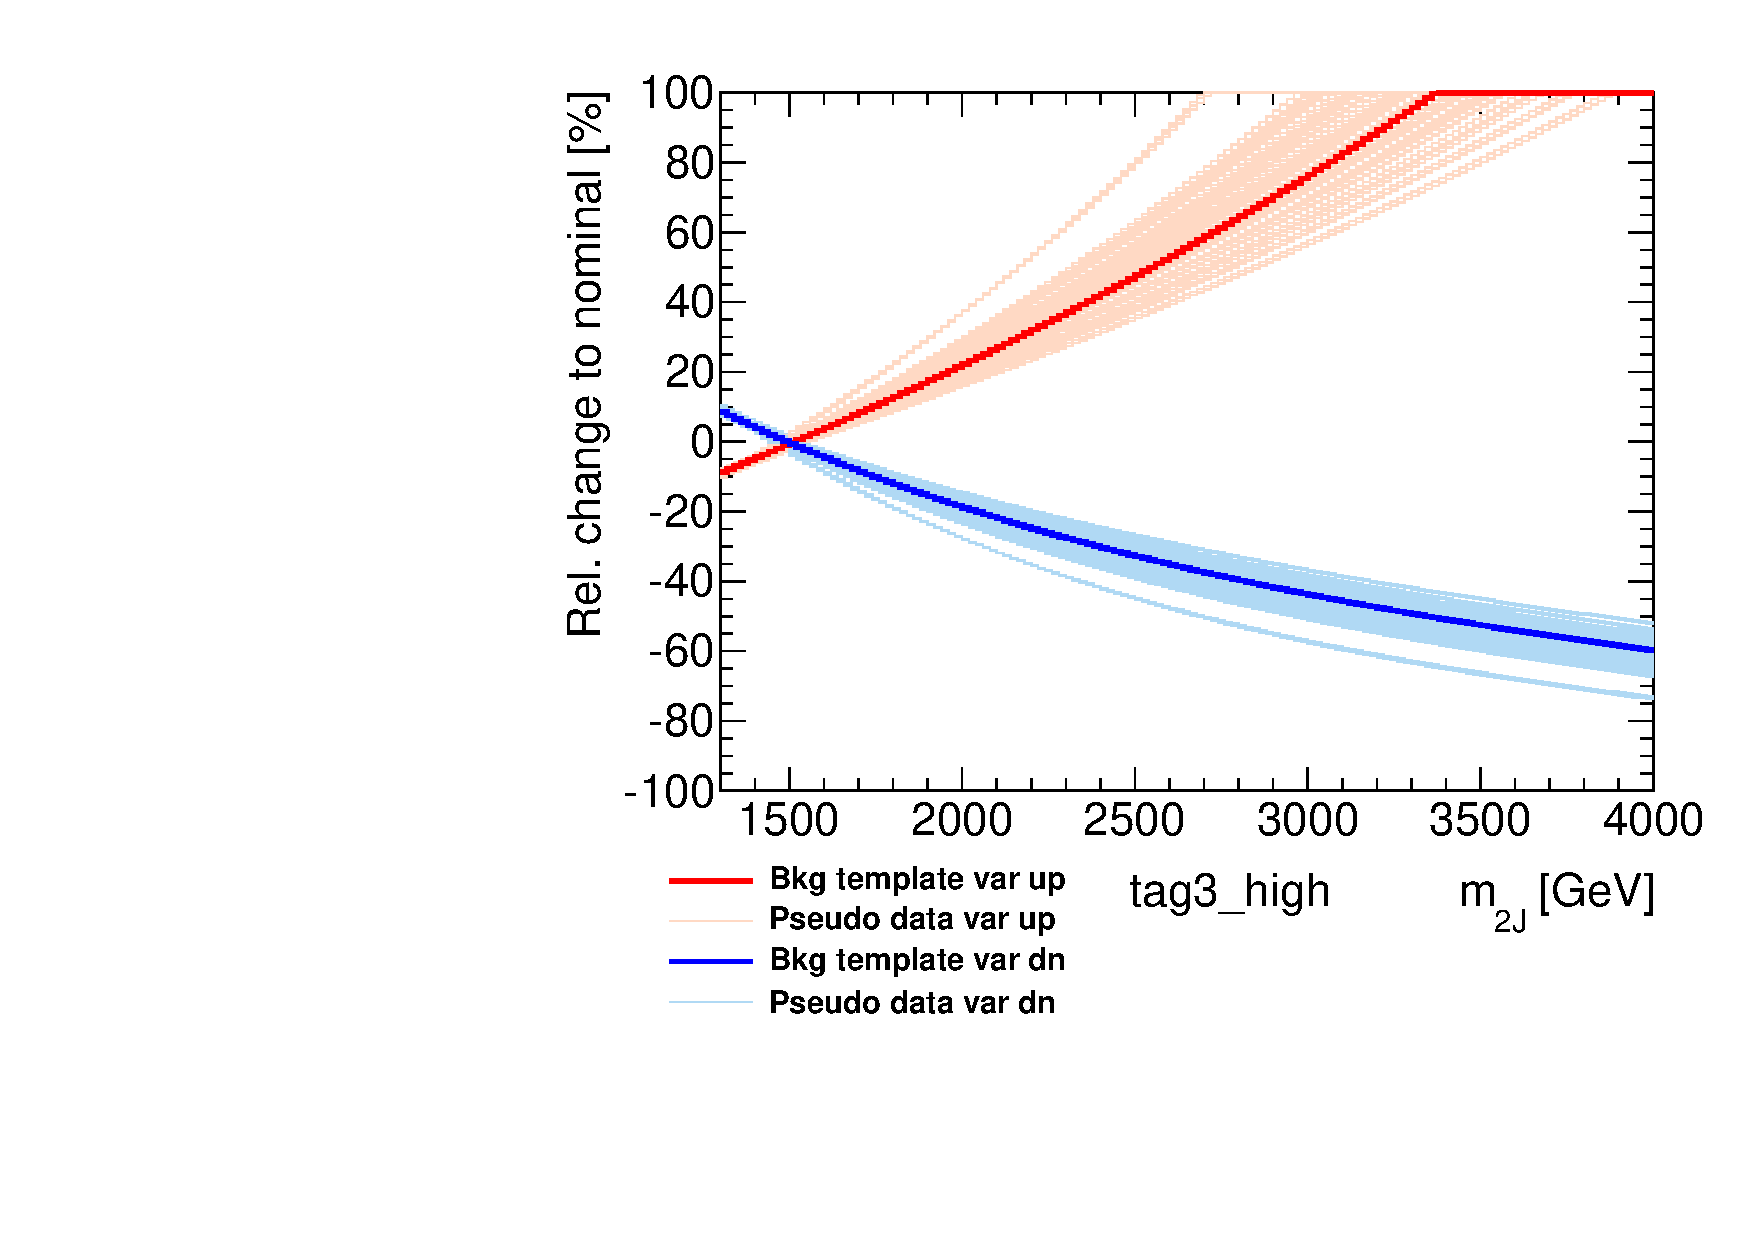
\includegraphics[angle=270, width=0.49\textwidth]{./figures/boosted/app-directfit/overlay_eigenvar2_tag3_high.pdf} }
\caption{Visualization of the eigenvariations for the 3b high mass category (function has 2 parameters). (a) shows variation 1 and (b) Var2.}
\label{fig:directfit:eigenvar3bhigh}
\end{center}
\end{figure*}

\begin{figure*}[htbp!]
\begin{center}
\subfloat[]{ 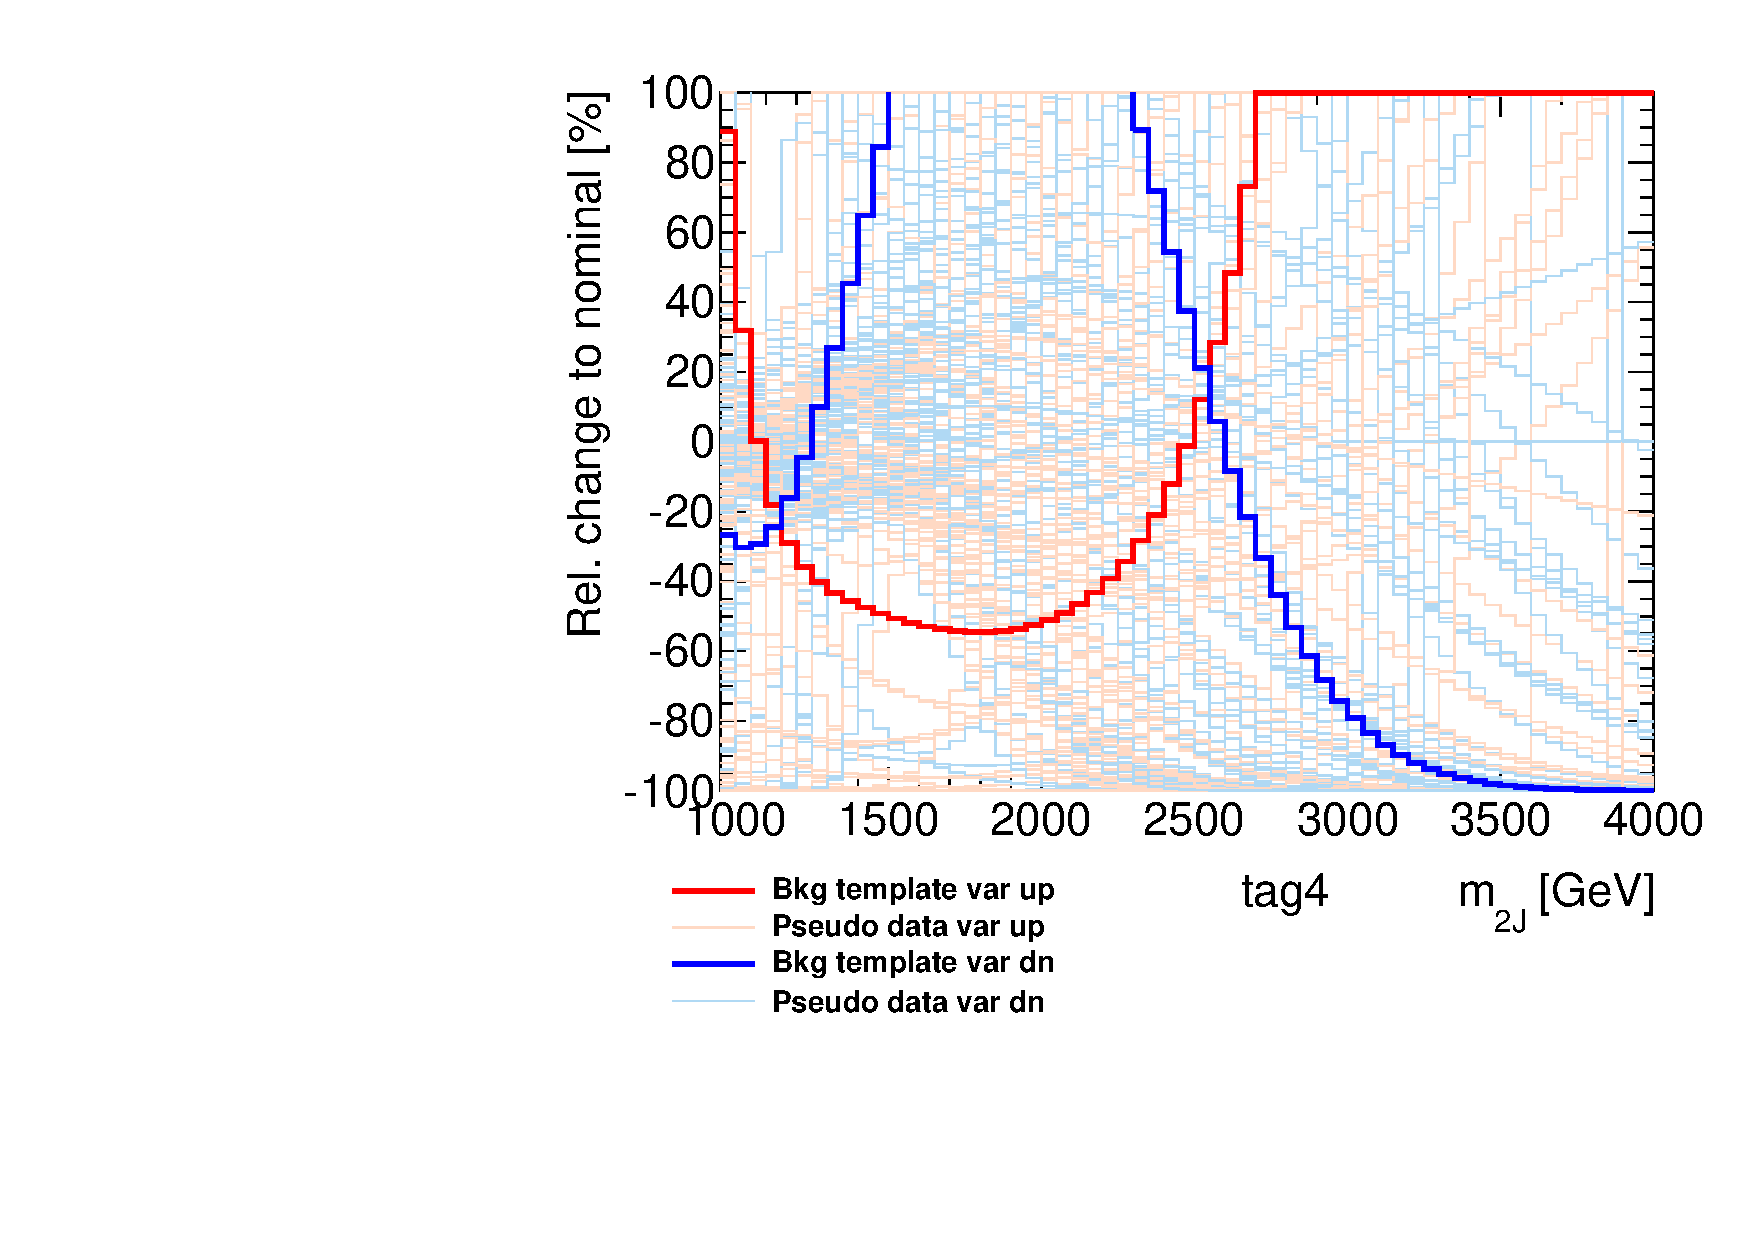
\includegraphics[angle=270, width=0.49\textwidth]{./figures/boosted/app-directfit/overlay_eigenvar1_tag4.pdf} }
\subfloat[]{ 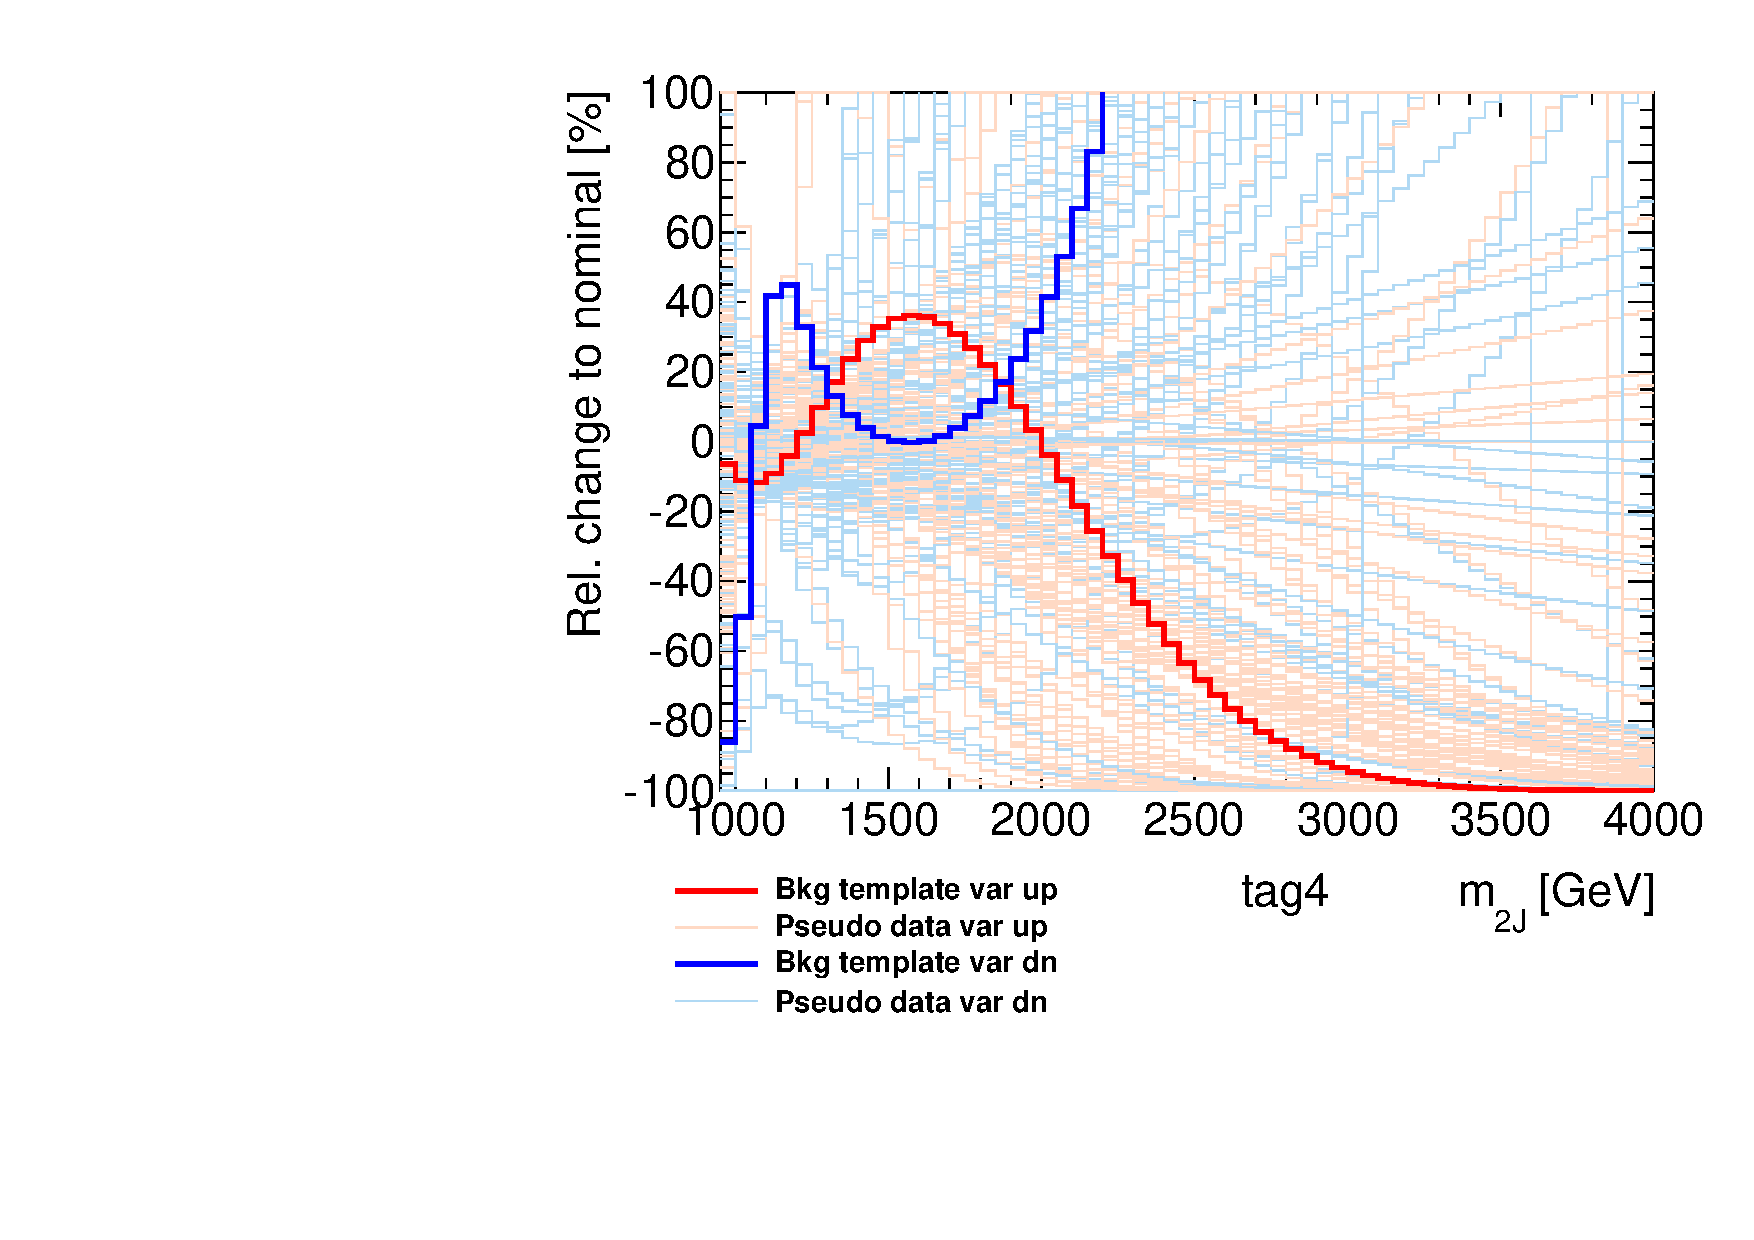
\includegraphics[angle=270, width=0.49\textwidth]{./figures/boosted/app-directfit/overlay_eigenvar2_tag4.pdf} } \\
\subfloat[]{ 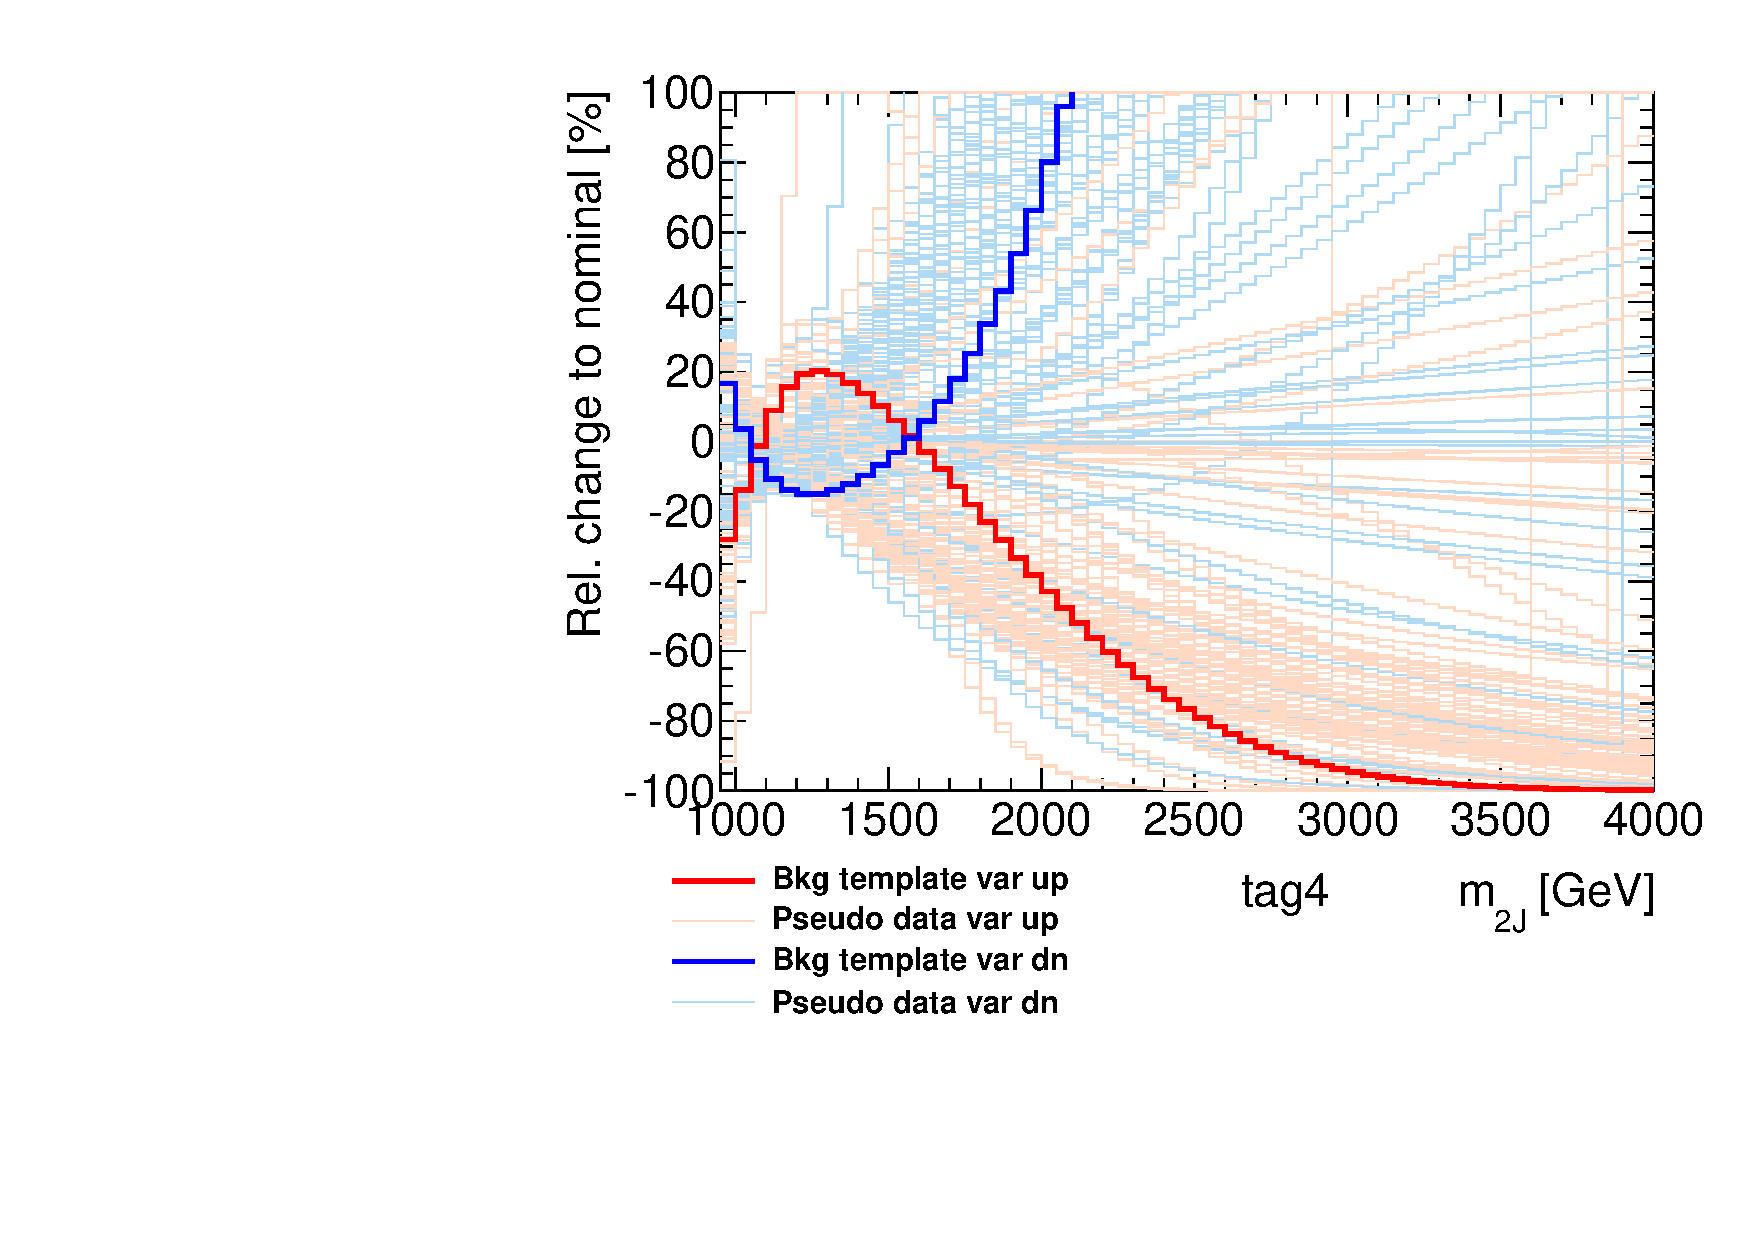
\includegraphics[angle=270, width=0.49\textwidth]{./figures/boosted/app-directfit/overlay_eigenvar3_tag4.pdf} }
\subfloat[]{ 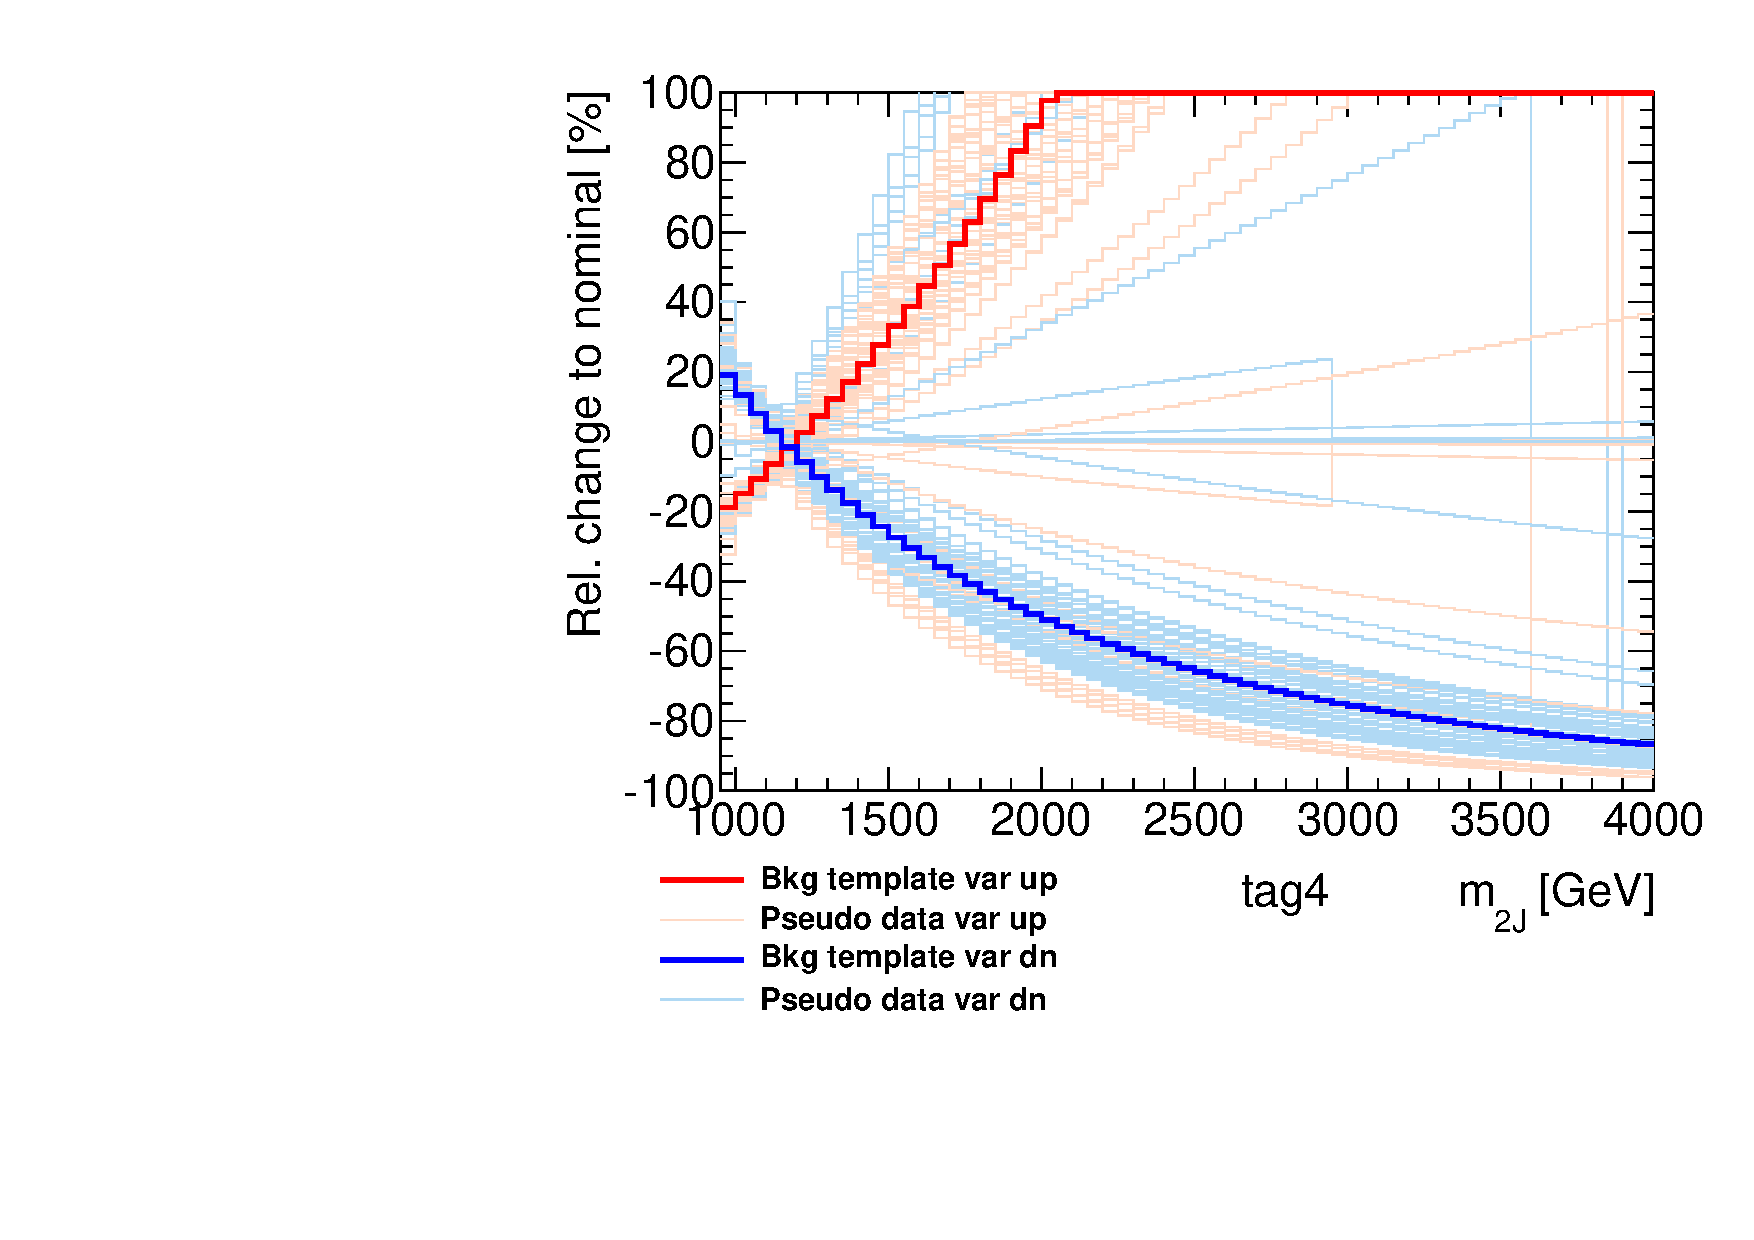
\includegraphics[angle=270, width=0.49\textwidth]{./figures/boosted/app-directfit/overlay_eigenvar4_tag4.pdf} }
\caption{Visualization of the eigenvariations for the 4b category (function has 4 parameters). (a) shows variation 1, (b) Var2, (c) Var3 and (d) Var4.}
\label{fig:directfit:eigenvar4b}
\end{center}
\end{figure*}

In the next step, the toys are used to build workspaces (one for each toy), and to fit the parameters of the model to the pseudo-data. The parameters are the signal strength $mu$, the nuisance parameters connected to the eigenvariations, and the nuisance parameters connected to the spurious signal uncertainty. For the signal, only the luminosity is considered. Log-normal constraints are used for all constrained parameters. Only $\mu$ is freely floating. Since the 4b category does not have enough statistics, it is not considered here. 


\subsection{Complete fit model and sensitivity}

To asess the sensitivity, workspaces are created from the histogram templates. This is done using RooFit, HistFactory is not used due to limited flexibility. The parameter of interest is the signal strength $\mu$, which scales the signal yield. If it is 0, it means no signal. All other parameters are constrained with Log-Normals. The nuisance parameters are the ones connected to the eigenvariations, the spurious signal, and the luminosity uncertainty (which acts only on the signal). The eigenvariations are collected into an instance of the class PiecewiseInterpolation, which is also used in HistFactory (but here it is used outside of HistFactory). The luminosity is treated correlated across the categories. The spurios signal is treated uncorrelated, ie. there is one NP for each category. The eigenvariations are obtained from the high-stat background-templates. The 4b category is not considered in this study.

The pulls and correlations of the floating parameters are displayed for Graviton mass of 1200 GeV in Fig.~\ref{fig:directfit:asimov1200}, for 2000 GeV using the low mass function in Fig.~\ref{fig:directfit:asimov2000_low}, and for 3000 GeV in Fig.~\ref{fig:directfit:asimov3000}. These fits are a combination of the 2bs and 3b categories. The parameters behave normally, there are no over constraints, and no significant correlations except at 1200 GeV, where there is a 50\% anti-correlation between the 3rd variation and the signal strength. As can be seen in Fig.~\ref{fig:directfit:eigenvar3blow} (c), this variation leads to an increase of the background around 1200 GeV, which probably explains this anti-correlation.

\begin{figure*}[htbp!]
\begin{center}
\subfloat[]{ 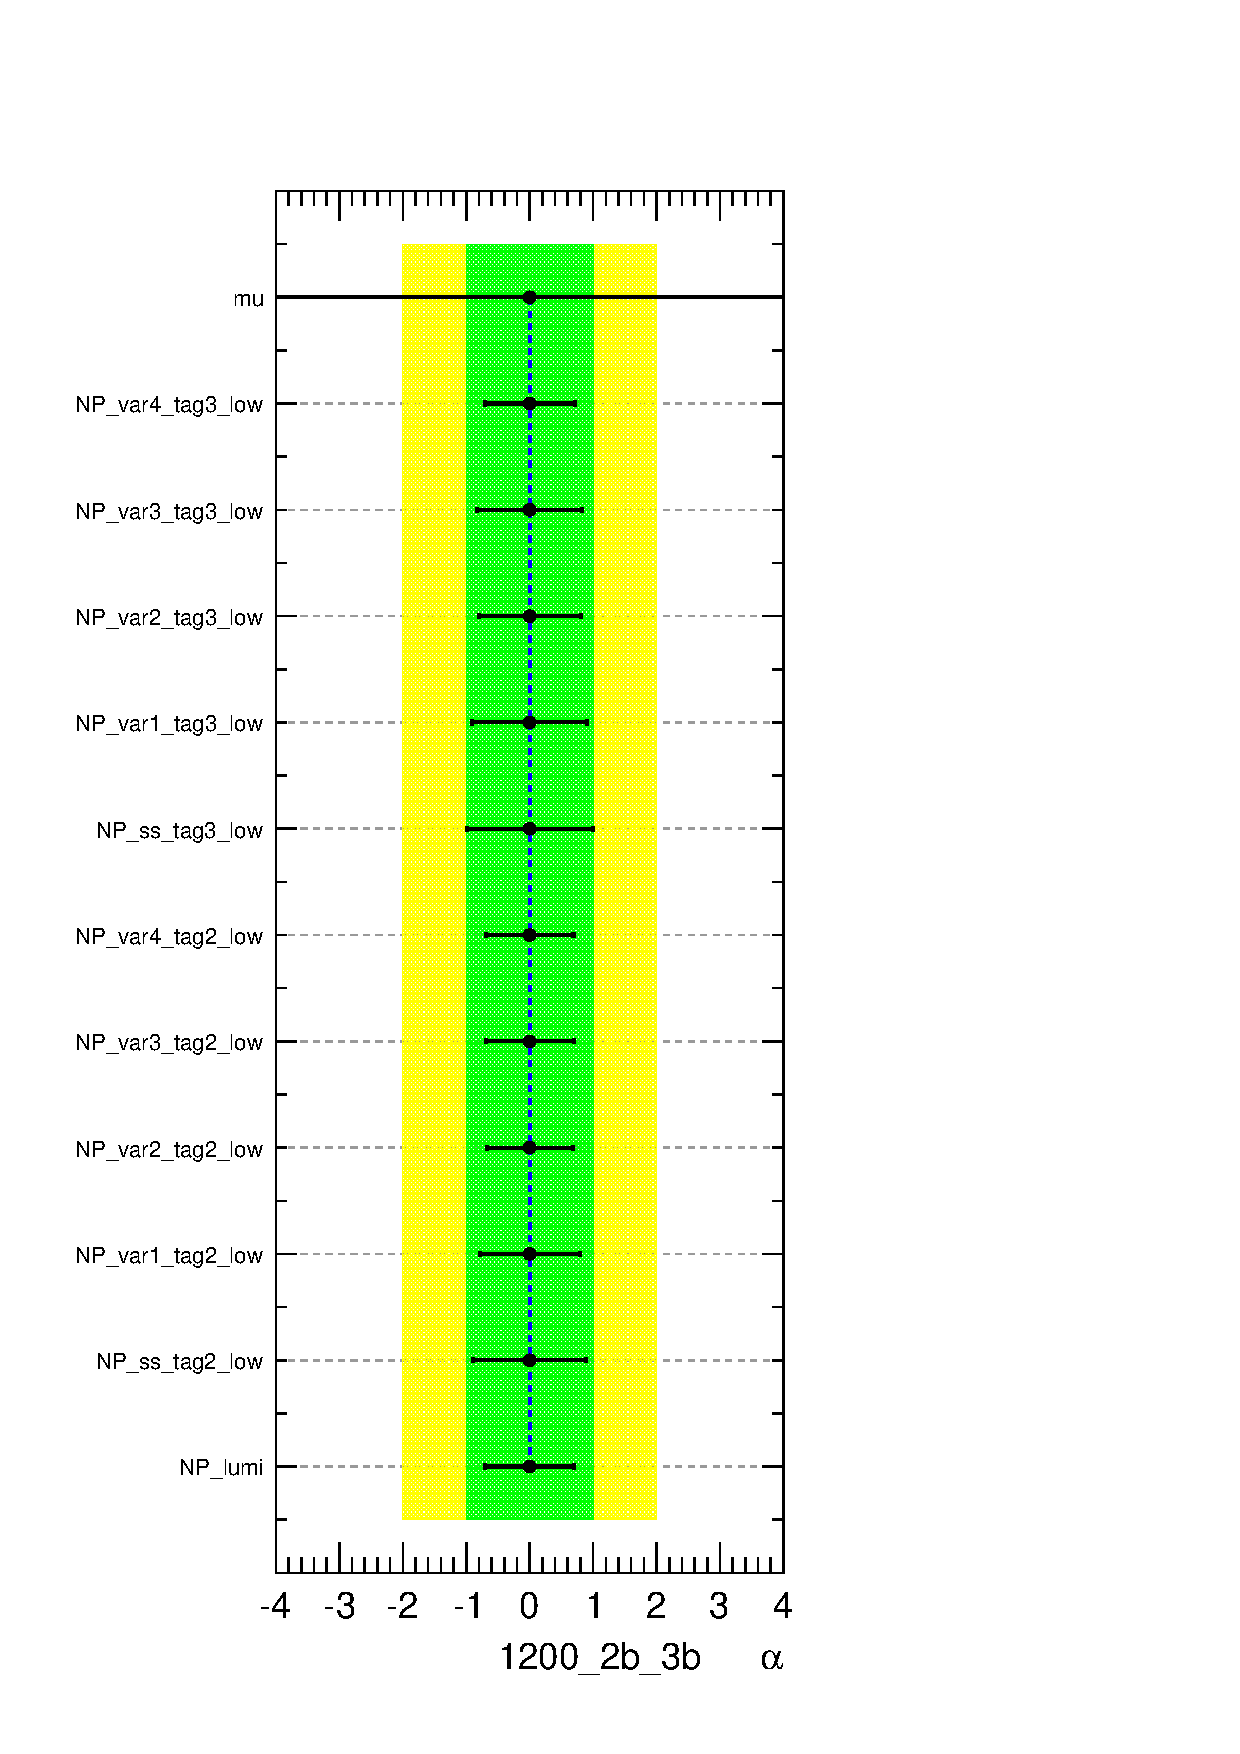
\includegraphics[angle=270, width=0.32\textwidth]{./figures/boosted/app-directfit/pulls_1200_2b_3b_asimov.pdf} }
\subfloat[]{ 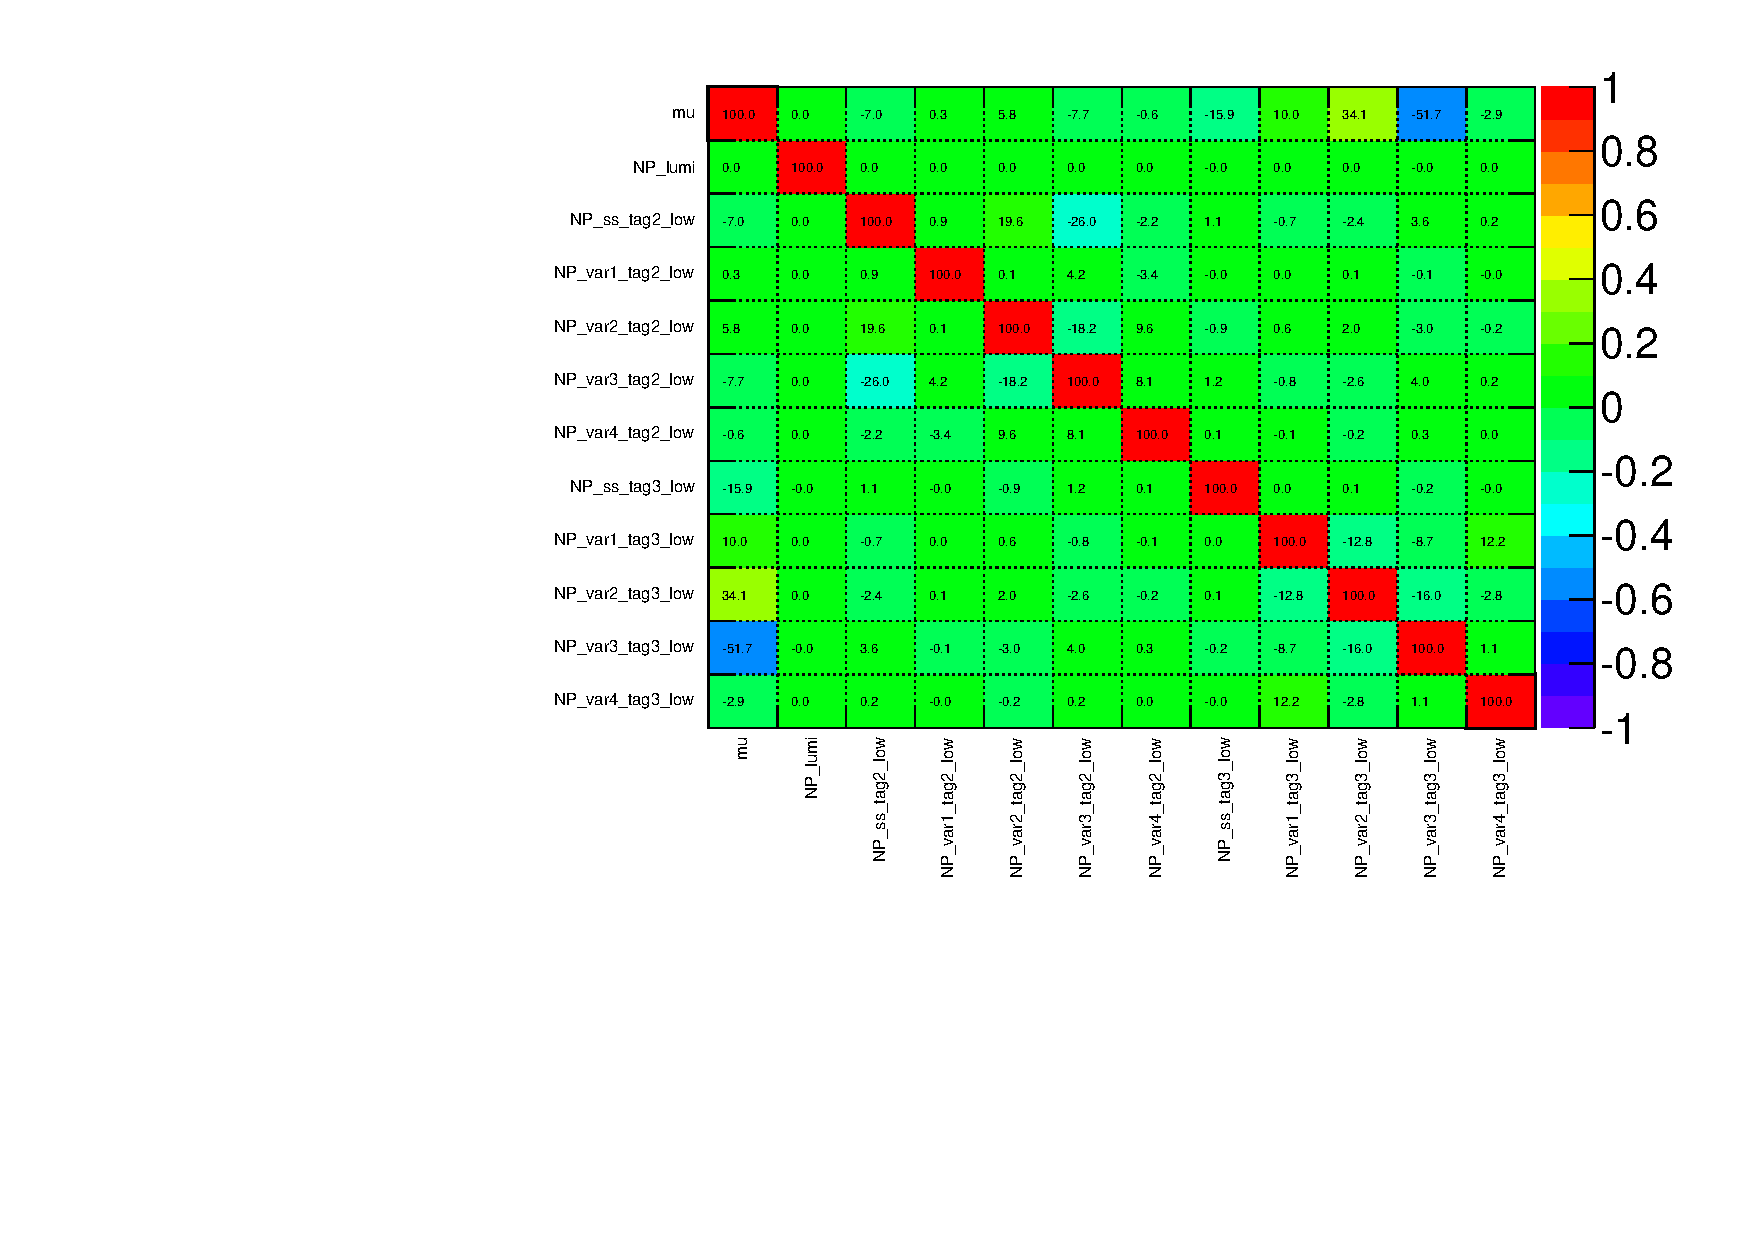
\includegraphics[angle=270, width=0.65\textwidth]{./figures/boosted/app-directfit/corr_1200_2b_3b_asimov.pdf} }
\caption{Asimov fit to the 1200 GeV mass point, showing (a) pulls and (b) correlations of the parameters.}
\label{fig:directfit:asimov1200}
\end{center}
\end{figure*}

\begin{figure*}[htbp!]
\begin{center}
\subfloat[]{ 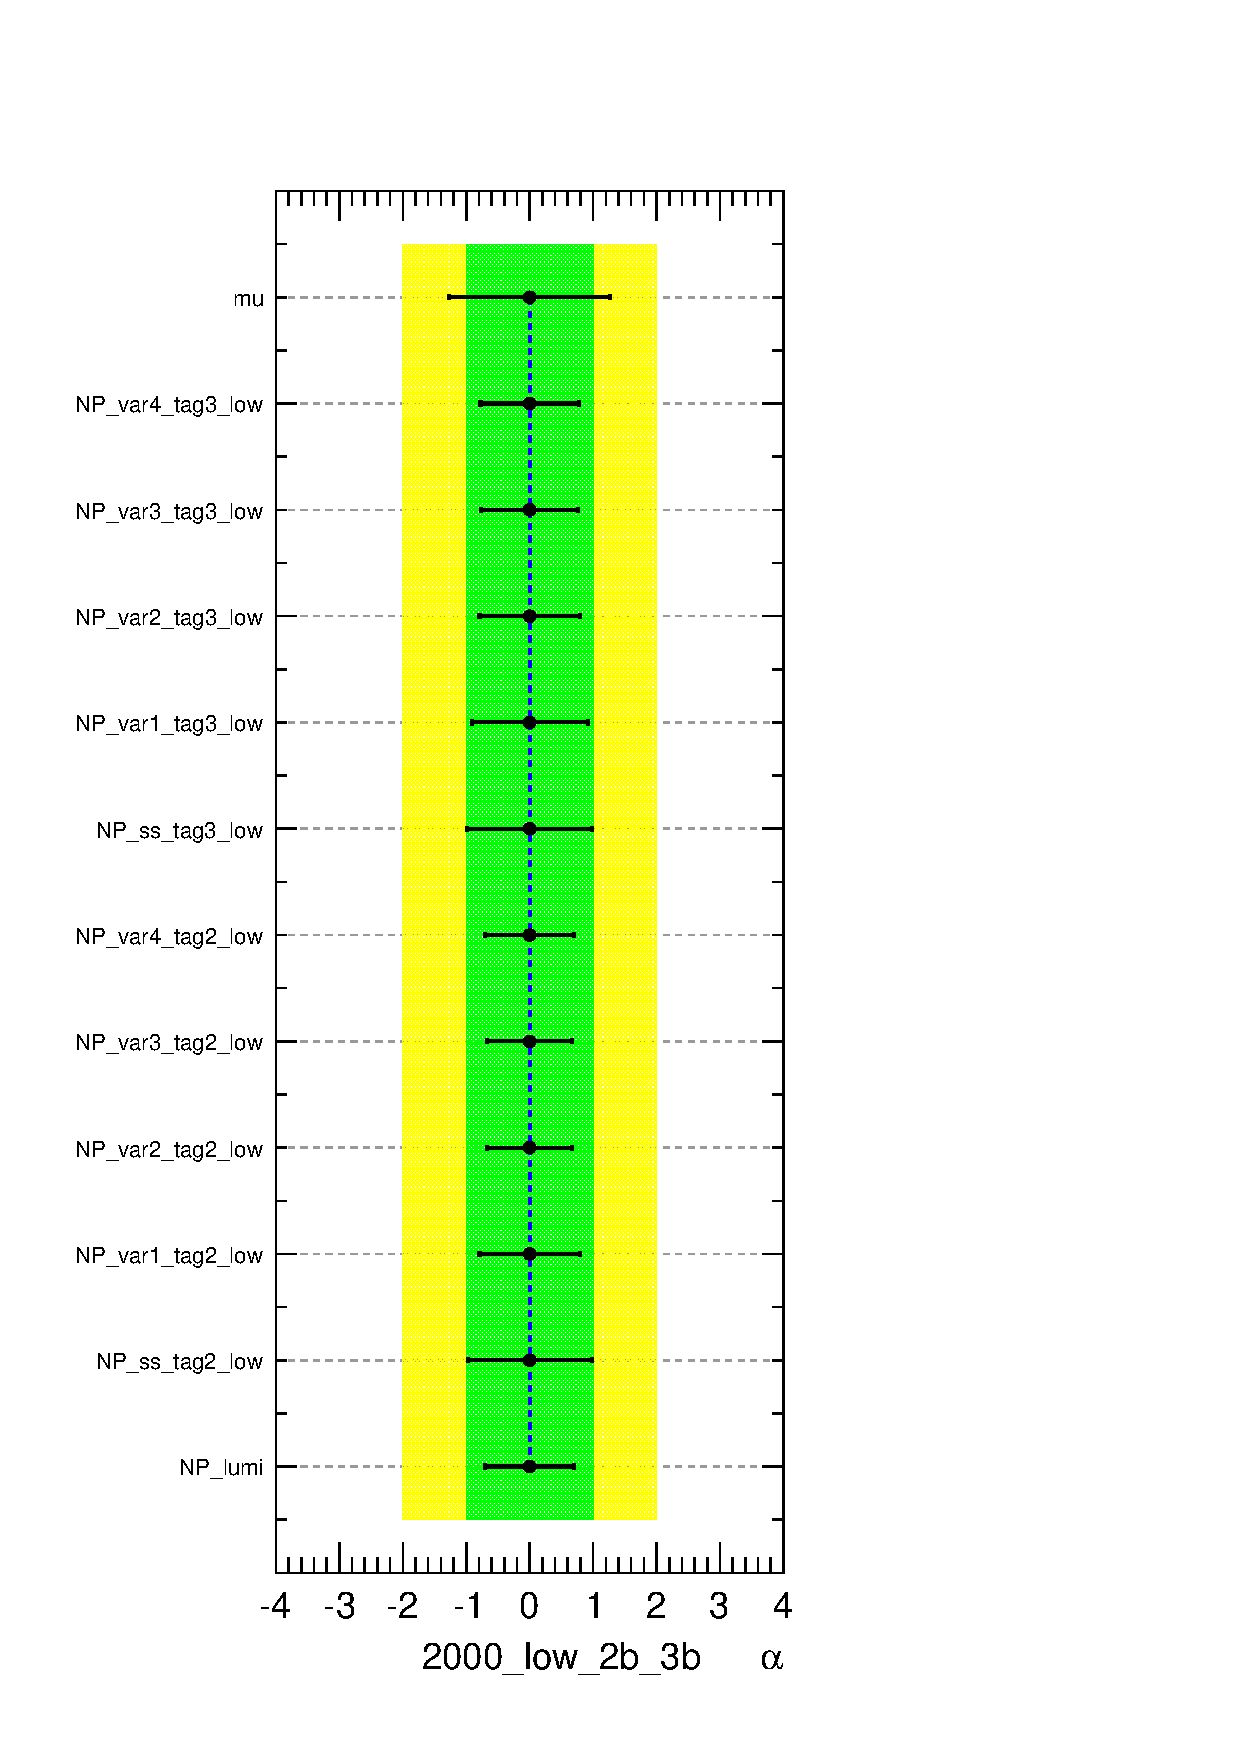
\includegraphics[angle=270, width=0.32\textwidth]{./figures/boosted/app-directfit/pulls_2000_low_2b_3b_asimov.pdf} }
\subfloat[]{ 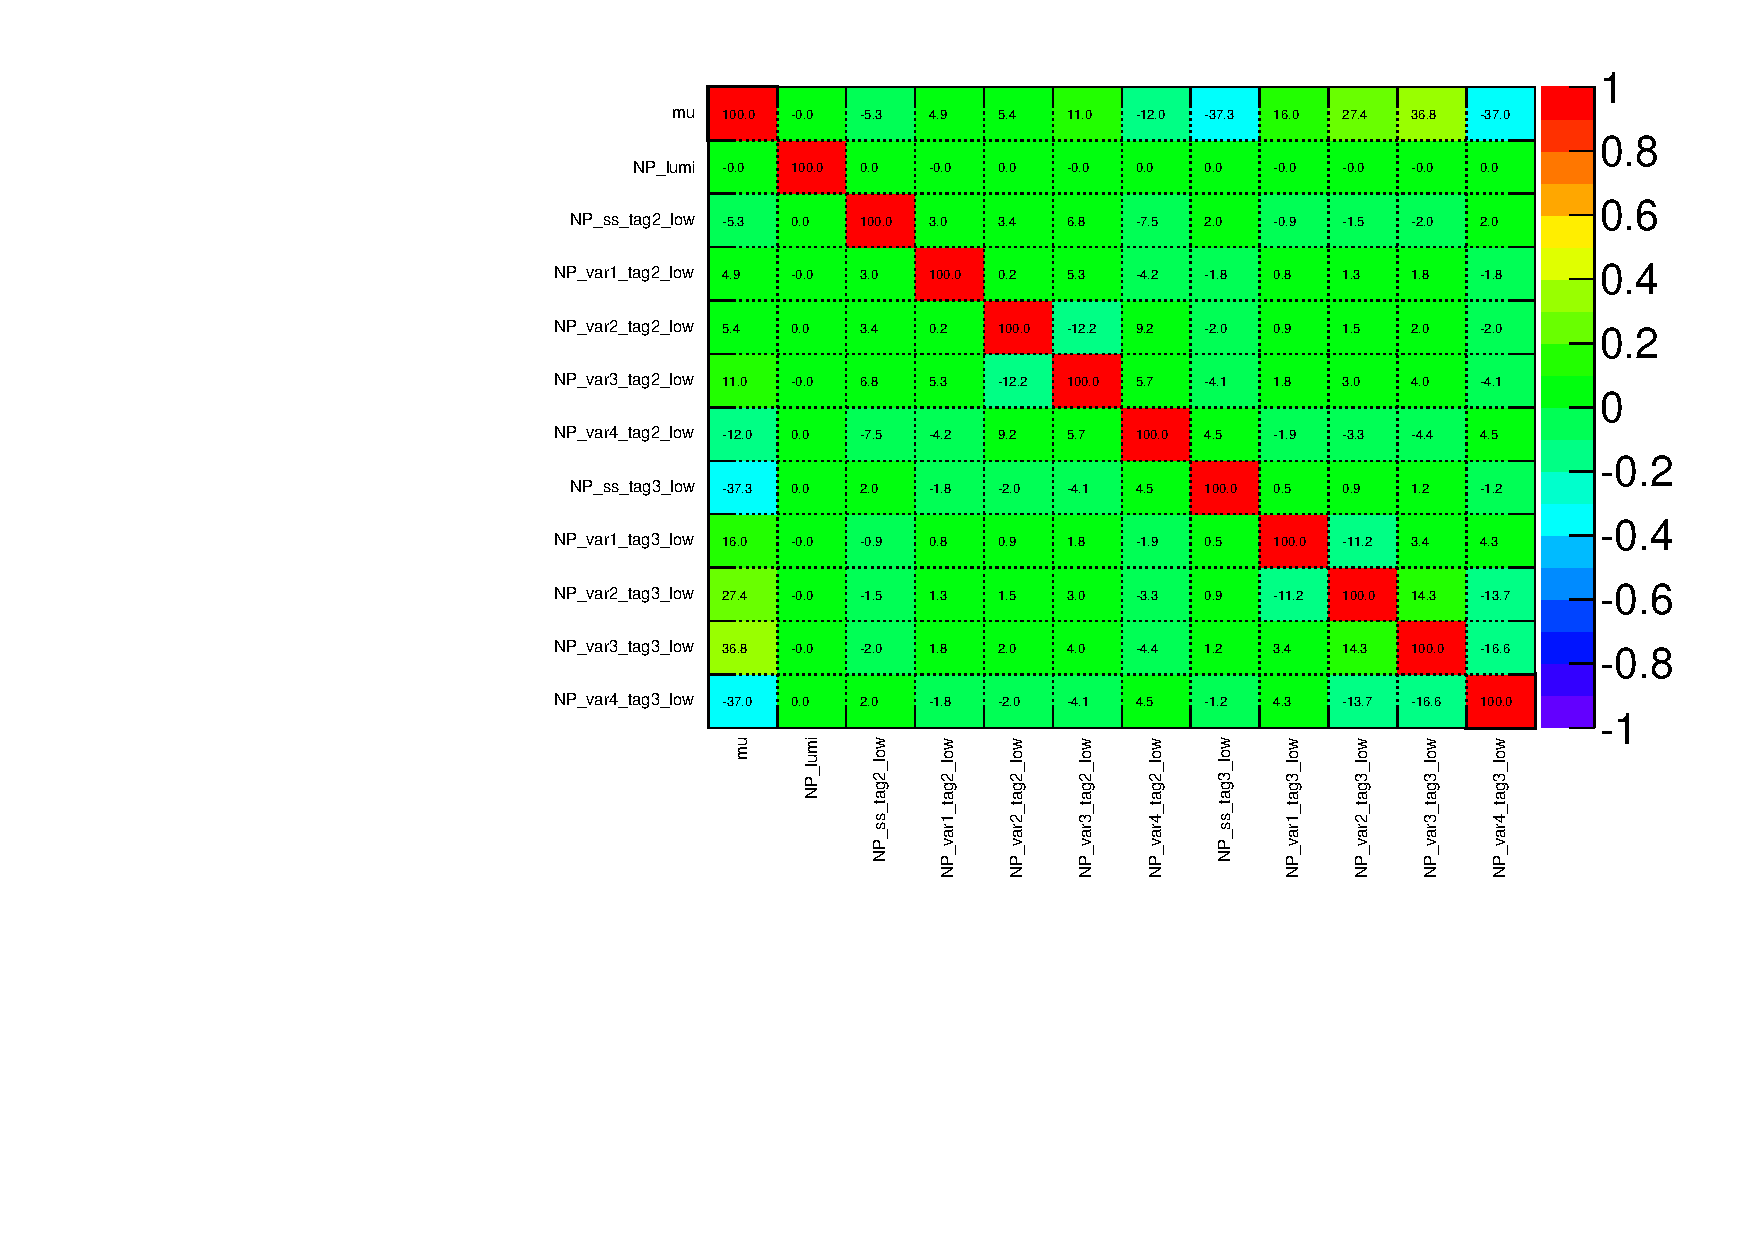
\includegraphics[angle=270, width=0.65\textwidth]{./figures/boosted/app-directfit/corr_2000_low_2b_3b_asimov.pdf} }
\caption{Asimov fit to the 2000 GeV mass point using the low mass functions, showing (a) pulls and (b) correlations of the parameters.}
\label{fig:directfit:asimov2000_low}
\end{center}
\end{figure*}

\begin{figure*}[htbp!]
\begin{center}
\subfloat[]{ 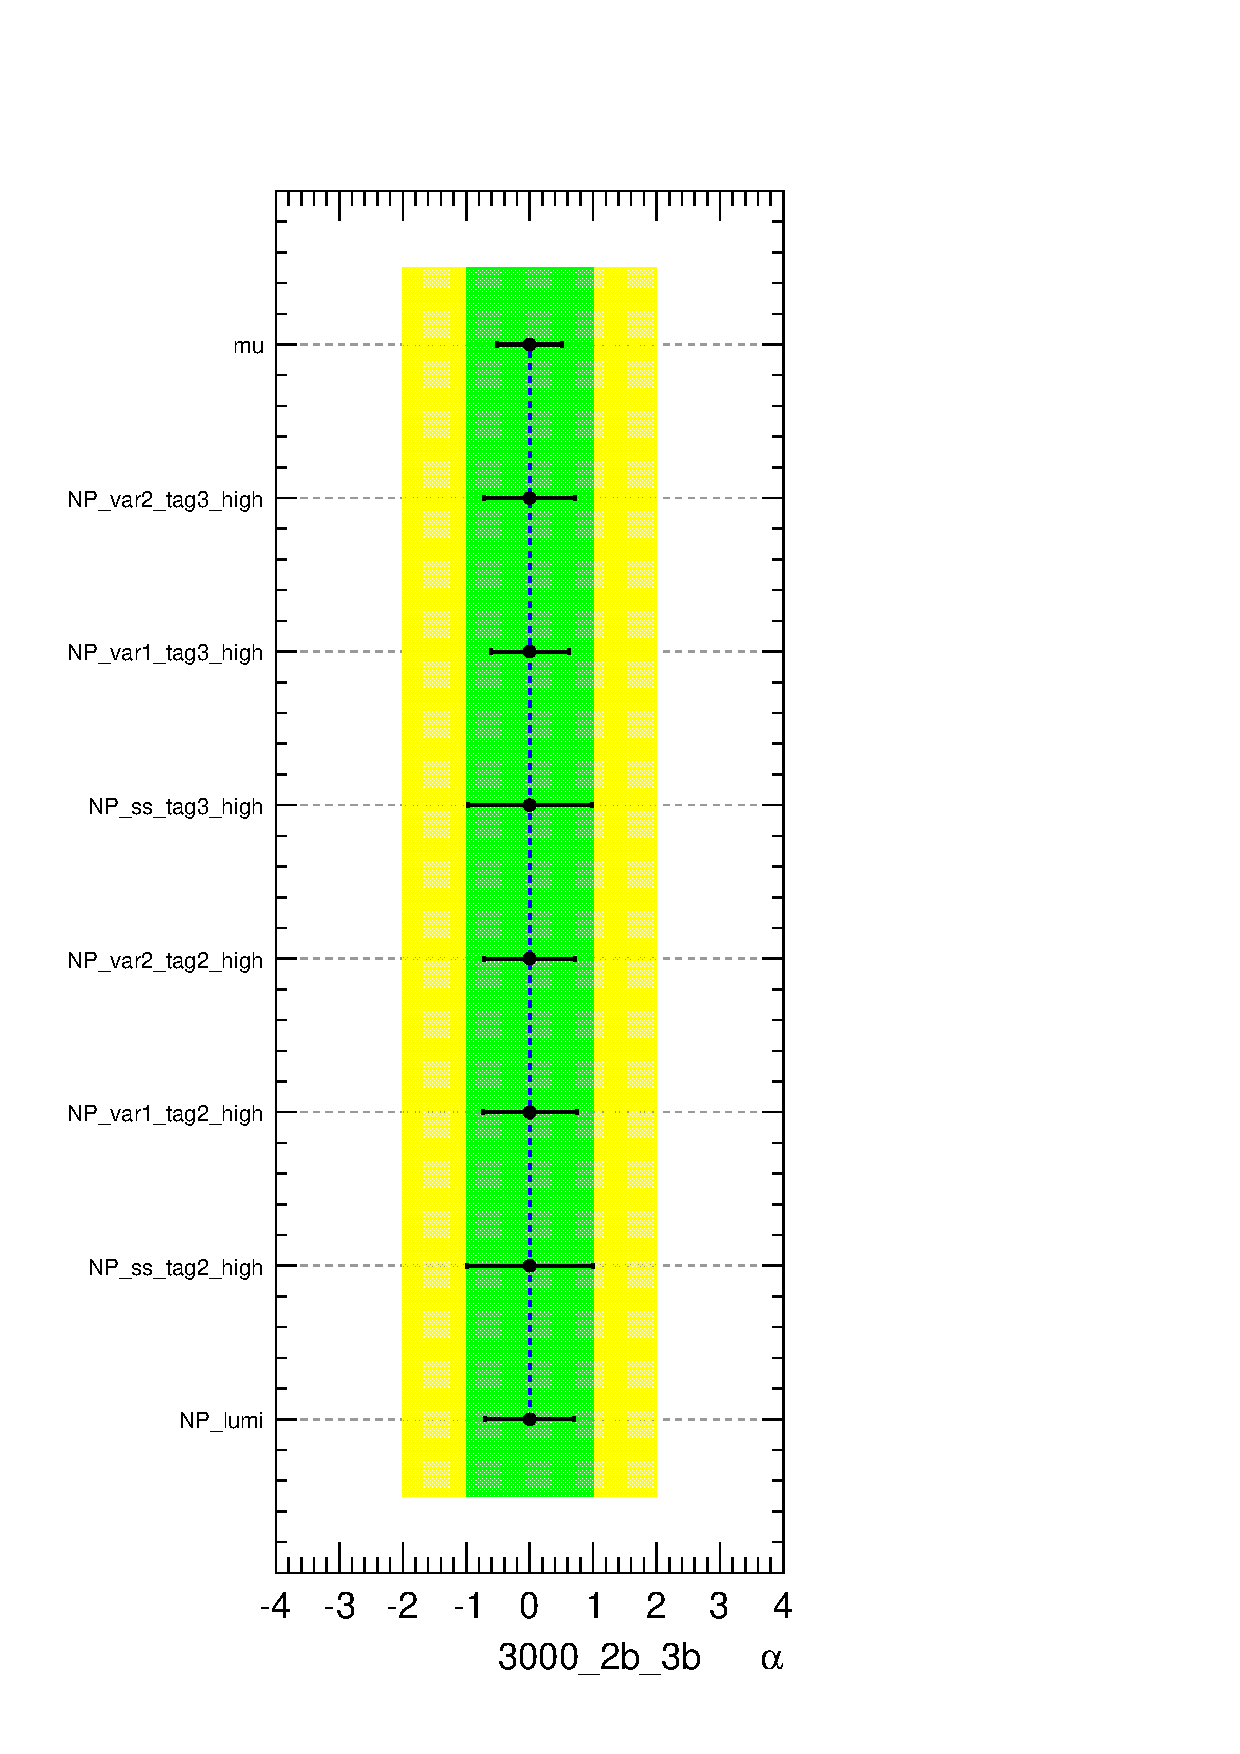
\includegraphics[angle=270, width=0.32\textwidth]{./figures/boosted/app-directfit/pulls_3000_2b_3b_asimov.pdf} }
\subfloat[]{ 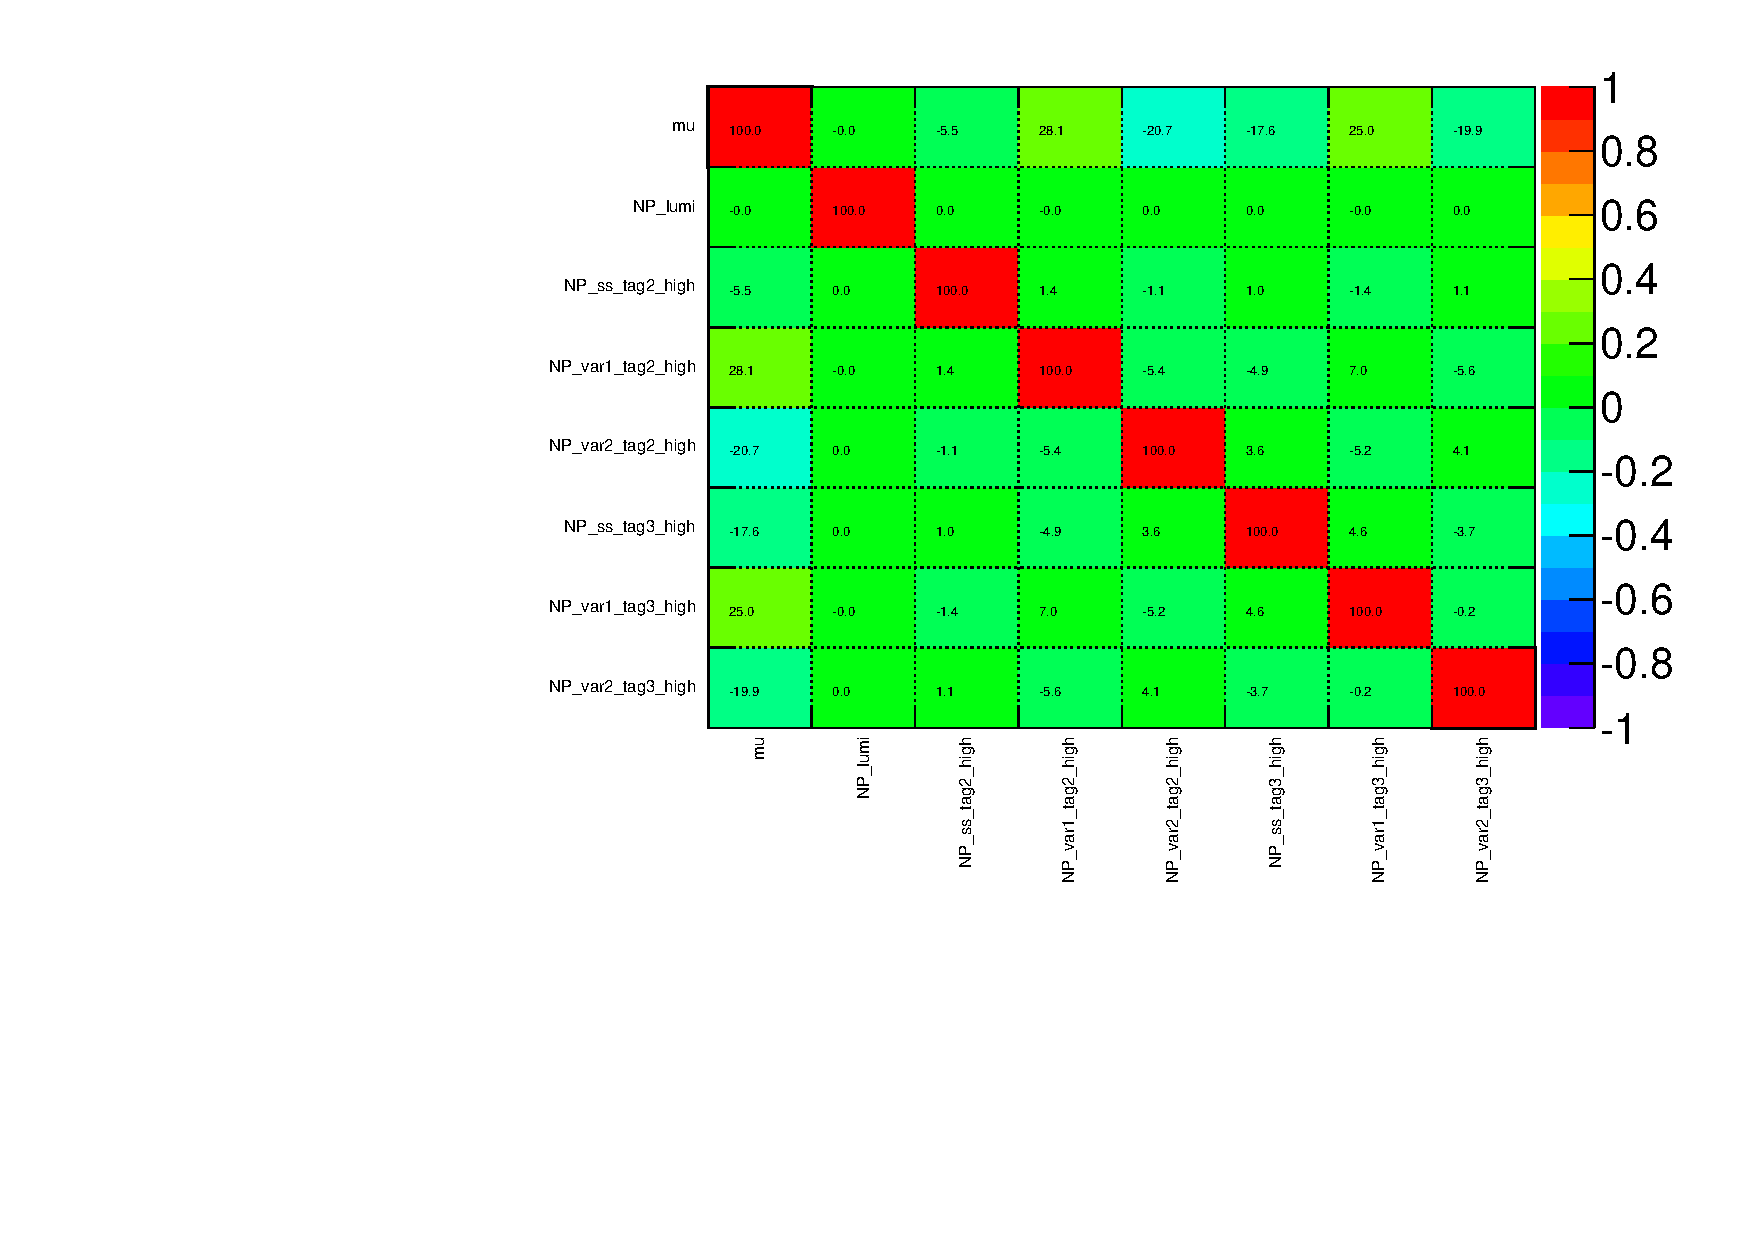
\includegraphics[angle=270, width=0.65\textwidth]{./figures/boosted/app-directfit/corr_3000_2b_3b_asimov.pdf} }
\caption{Asimov fit to the 3000 GeV mass point, showing (a) pulls and (b) correlations of the parameters.}
\label{fig:directfit:asimov3000}
\end{center}
\end{figure*}

The limits are evaluated separately for 2bs and 3b, to allow a comparison with the nominal analysis based on the muQCD method. They are displayed in Fig.~\ref{fig:directfit:limits}. A comparison to the limit from Patrick, sent by email on the 19th of June 2017, yields that the limits are comparable at medium and high mass for both categories, but the direct fit limits are worse at low mass, by about a factor 1.4 at 1200 GeV.

\begin{figure*}[htbp!]
\begin{center}
\subfloat[]{ \includegraphics[angle=270, width=0.49\textwidth]{./figures/boosted/app-directfit/limit_2b.pdf} }
\subfloat[]{ \includegraphics[angle=270, width=0.49\textwidth]{./figures/boosted/app-directfit/limit_3b.pdf} }
\caption{The limit obtained with the direct fit method, for the categories (a) 2bs and (b) 3b. The crack at 2000 GeV comes from the change of the fit function.}
\label{fig:directfit:limits}
\end{center}
\end{figure*}
